\documentclass{template/openetcs_report}
% Use the option "nocc" if the document is not licensed under Creative Commons
%\documentclass[nocc]{template/openetcs_article}
\usepackage{rotating,url,color}
\usepackage[hidelinks]{hyperref}
\graphicspath{{./template/}{.}{./images/}}
\begin{document}
\frontmatter
\project{openETCS}

%Please do not change anything above this line
%============================
% The document metadata is defined below

%assign a report number here
\reportnum{OETCS/WP7/O7.1.3\_O7.1.7~--~00/02}

%define your workpackage here
\wp{Work-Package 7: ``Primary tool chain''}

%set a title here
\title{Evaluation of the models and tools against the WP2 requirements }

%set a subtitle here
\subtitle{List of criteria on means, models and tools and results on the benchmark}

%set the date of the report here
\date{May 2013}

%define a list of authors and their affiliation here

\author{Marielle Petit-Doche}
\affiliation{Systerel}

% define the coverart
\coverart[width=350pt]{chart}
 
%define the type of report
\reporttype{Definition}


\begin{abstract}
This document gives elements to evaluate the means of modeling and the associated tools according WP2 requirements. Evaluation on the models and tools of benchmark is also described.

\end{abstract}

%=============================
%Do not change the next three lines
\maketitle
\tableofcontents
\listoffiguresandtables
\newpage
%=============================


\begin{tabular}{|p{4.4cm}|p{8.7cm}|}
\hline
\multicolumn{2}{|c|}{Document information} \\
\hline
Work Package &  WP7  \\
Deliverable ID or doc. ref. & O7.3.1\_O7.1.7\\
\hline
Document title & Evaluation of the models and toolsagainst the WP2 requirements \\
Document version & 00.02 \\
Document authors (org.)  & Marielle Petit-Doche (Systerel)  \\
\hline
\end{tabular}

\begin{tabular}{|p{4.4cm}|p{8.7cm}|}
\hline
\multicolumn{2}{|c|}{Review information} \\
\hline
Last version reviewed & 00.01 \\
\hline
Main reviewers & Uwe Steinke (Siemens) \\
 & Armand Nachef (CEA) \\
 & Cyril Cornu (All4Tech) \\
 & Alexandre Ginisty (All4Tech) \\
 & Mathieu Perrin (CEA) \\
\hline
\end{tabular}

\begin{tabular}{|p{2.2cm}|p{4cm}|p{4cm}|p{2cm}|}
\hline
\multicolumn{4}{|c|}{Approbation} \\
\hline
  &  Name & Role & Date   \\
\hline  
Written by    &  Marielle Petit-Doche & WP7-T7.1 Sub-Task Leader  & \\
\hline
Approved by & Michael Jastram & WP7 leader & \\
\hline
\end{tabular}

\begin{tabular}{|p{2.2cm}|p{2cm}|p{3cm}|p{5cm}|}
\hline
\multicolumn{4}{|c|}{Document evolution} \\
\hline
Version &  Date & Author(s) & Justification  \\
\hline  
00.01 & 19/04/2013 & M. Petit-Doche &  Document creation by merging O7.1.3 and O7.1.7 \\
\hline  
00.02 & 02/05/2013 & M. Petit-Doche &  Review remarks \\
& & & Tool evaluation matrix \\
\hline  
\end{tabular}

% The actual document starts below this line
%=============================


%%%%%%%%%%%%%%%%%%%%%%%%%%%%%%%%%%%%%%%%%%%%%%%%%%%%%%%%%%%%%%
%%%              My macros (=> Sylvain Baro)               %%%
%%%%%%%%%%%%%%%%%%%%%%%%%%%%%%%%%%%%%%%%%%%%%%%%%%%%%%%%%%%%%%
\newcommand{\tbd}{\colorbox{cyan}{\%\%To Be Defined\%\%}}
\newcommand{\tbc}{\colorbox{cyan}{\%\%To Be Confirmed\%\%}}
\newcommand{\todo}[1]{\colorbox{cyan}{\%\%{#1}\%\%}}
\newlength{\origindent}

\newenvironment{issue}{
        \begin{quote}
        \begin{itshape}Open Issue.
}{
        \end{itshape}
        \end{quote}
}

\newenvironment{comment}{
        \begin{quote}
        \begin{itshape}Comment.
}{
        \end{itshape}
        \end{quote}
}

\newenvironment{justif}{
        \begin{quote}
        \begin{itshape}Justification.
}{
        \end{itshape}
        \end{quote}
}


\newenvironment{author_comment}{
        \begin{quote}
        \begin{itshape}\textcolor{green}{Author.}
}{
        \end{itshape}
        \end{quote}
}


\newenvironment{assessor1}{
        \begin{quote}
        \begin{itshape} \textcolor{blue}{Assessor 1.}
}{
        \end{itshape}
        \end{quote}
}


\newenvironment{assessor2}{
        \begin{quote}
        \begin{itshape}\textcolor{magenta}{Assessor 2.}
}{
        \end{itshape}
        \end{quote}
}
% %% Requirements.


\newcounter{reqnum}
\setcounter{reqnum}{0}
\newcounter{subreqnum}
\newcounter{subsubreqnum}
\newlength{\partopbuf}
\newlength{\topbuf}

% Automated numbering versions of the macros
\newcommand{\req}[1]{\addtocounter{reqnum}{1} \setcounter{subreqnum}{0}
	\setlength{\partopbuf}{\partopsep}
	\setlength{\partopsep}{0pt}
	\setlength{\topbuf}{\topsep}
	\setlength{\topsep}{0pt}
	\begin{description}\item[{\small\reqt-X-\thereqnum}] #1\end{description}
	\setlength{\partopsep}{\partopbuf}
	\setlength{\topsep}{\topbuf}	
	}

\newcommand{\subreq}[1]{
	\addtocounter{subreqnum}{1} \setcounter{subsubreqnum}{0}
	\setlength{\partopbuf}{\partopsep}
	\setlength{\partopsep}{0pt}
	\setlength{\topbuf}{\topsep}
	\setlength{\topsep}{0pt}
	\begin{description}\addtolength{\leftmargin}{1cm}
	\item[{\small\reqt-X-\thereqnum.\thesubreqnum}] #1
	\addtolength{\leftmargin}{-1cm}\end{description}
	\setlength{\partopsep}{\partopbuf}
	\setlength{\topsep}{\topbuf}
}

\newcommand{\subsubreq}[1]{
	\addtocounter{subsubreqnum}{1}
	\setlength{\partopbuf}{\partopsep}
	\setlength{\partopsep}{0pt}
	\setlength{\topbuf}{\topsep}
	\setlength{\topsep}{0pt}
	\begin{description}\addtolength{\leftmargin}{1cm}
	\item[{\small\reqt-X-\thereqnum.\thesubreqnum.\thesubsubreqnum}] #1
	\addtolength{\leftmargin}{-1cm}\end{description}
	\setlength{\partopsep}{\partopbuf}
	\setlength{\topsep}{\topbuf}
}

% Fixed version of the commands
\newcommand{\reqfixed}[3]{\addtocounter{reqnum}{1} \setcounter{subreqnum}{0}
	\setlength{\partopbuf}{\partopsep}
	\setlength{\partopsep}{0pt}
	\setlength{\topbuf}{\topsep}
	\setlength{\topsep}{0pt}
	\begin{description}\item[{\small\reqt-#1-#2}] #3\end{description}
	\setlength{\partopsep}{\partopbuf}
	\setlength{\topsep}{\topbuf}	
	}

\newcommand{\subreqfixed}[4]{
	\addtocounter{subreqnum}{1} \setcounter{subsubreqnum}{0}
	\setlength{\partopbuf}{\partopsep}
	\setlength{\partopsep}{0pt}
	\setlength{\topbuf}{\topsep}
	\setlength{\topsep}{0pt}
	\begin{description}\addtolength{\leftmargin}{1cm}
	\item[{\small\reqt-#1-#2.#3}] #4
	\addtolength{\leftmargin}{-1cm}\end{description}
	\setlength{\partopsep}{\partopbuf}
	\setlength{\topsep}{\topbuf}
}

\newcommand{\subsubreqfixed}[5]{
	\addtocounter{subsubreqnum}{1}
	\setlength{\partopbuf}{\partopsep}
	\setlength{\partopsep}{0pt}
	\setlength{\topbuf}{\topsep}
	\setlength{\topsep}{0pt}
	\begin{description}\addtolength{\leftmargin}{1cm}
	\item[{\small\reqt-#1-#2.#3.#4}] #5
	\addtolength{\leftmargin}{-1cm}\end{description}
	\setlength{\partopsep}{\partopbuf}
	\setlength{\topsep}{\topbuf}
}

% Citation of the requirement

% Citation of the reference (for markup purpose)
\newcommand{\refreq}[1]{\textbf{#1}}

% Citation of the reference and text (for markup purpose)
% The purpose of this is to automatically replace the placeholder by the 
% full text. \fullrefreq{R-xxx}{} or \fullrefreq{R-xxx}{blabla} 
% will be replaced by \fullrefreq{R-xxx}{text of the R-xxx requirement} 
\newcommand{\fullrefreq}[2]{\textbf{#1}: \textrm{#2}}



\def\reqt{R-WP2/D2.3.0}
% Start here

\mainmatter

% Start here


\chapter{Introduction}


The aim of this document is to report the results of the evaluation of the means of description to model the requirements of SUBSET-026 concerning the on-board unit and their assocaited tools.

This evaluation task is part on work package WP7, task 1  "Primary tool Chain analyses and recommendations". According to the results of WP2, especially the OpenETCS process and the requirements on language, the aim of this task is to determine the best candidates to  produce models of the on-board units, following the OpenETCS process

This process is described in détail in D2.3 " Description of the openETCS process" and is summed up in the figure \ref{fig:main_process}.
 

 \begin{figure}
  \centering
  \fbox{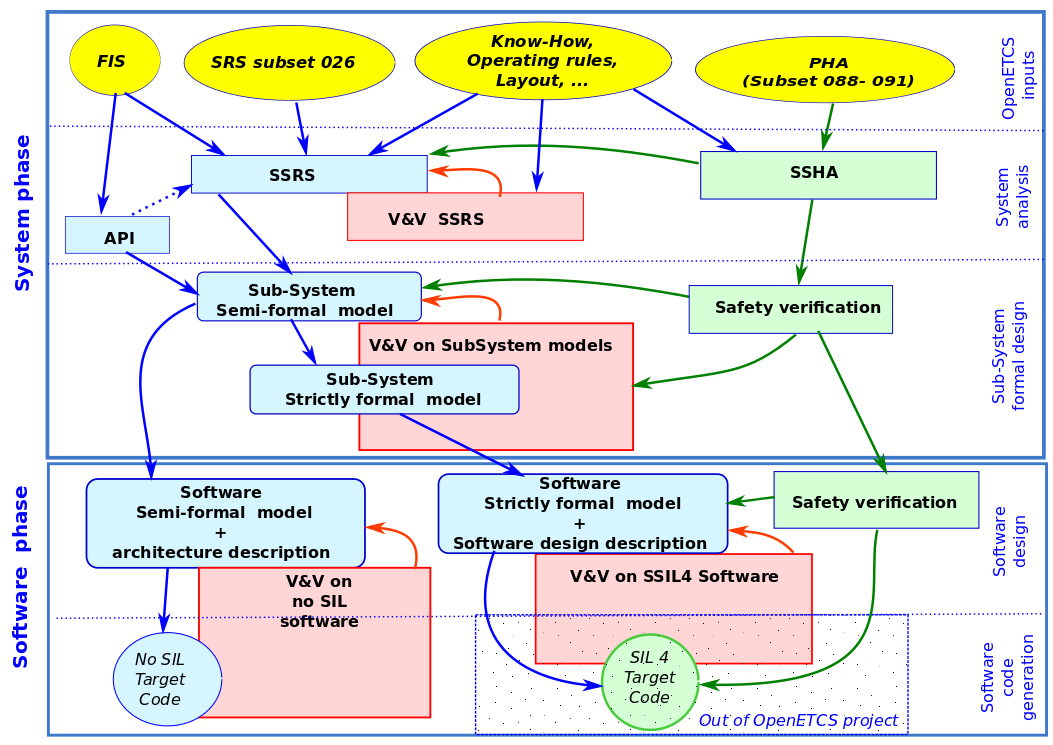
\includegraphics[scale=0.45]{WholeProcess.png}}
  \caption{Main OpenETCS process}
  \label{fig:main_process}
\end{figure}

Yellow elements are inputs, blue elements are part of the design process, red elements are verification and validation activities, green elements are safety activities. Each line (between dash or full blue lines) is a phase of the process, with a name on the right. 

The second section of this document provides a template to describe the means and tools and a list of criteria according WP2 requirements on language, models and tools. The objectives of this description and criteria are to allow to determine the best means of description and associated tool for a given activities.

The third section resumes the results of the evaluation at the end of the benchmark activities.

In Appendix, a section is dedicated to each models produced during the benchmark activities :
\begin{itemize}
\item  CORE
\item  GOPRR
\item  ERTMSFormalSpecs
\item  SysML with Papyrus
\item  SysML with Entreprise Architect
\item  SCADE
\item  EventB with Rodin
\item  Classical B with Atelier B
\item  Petri Nets
\item  System C
\item  GNATprove
\end{itemize}

For each approach and tool, the initial  author of the evaluation is the partner in charge of the modelling. Two assessors, for each approaches,  are in charge of the review of the evaluation and can correct it or add comments.

Tool platform are not covered by this document but in an other output of WP7 :  O7.1.9 "Evaluation of each tool platform against WP2 requirements, independent of target tools".
Besides, Task 7.1 is focussing on design activities : despite that some means can provide verification artefacts for example,  tools and means for validation, verification, test generation,... are in the scope of task 2 and will be analysed later.



\chapter{Templates}
\label{sec:templates}

\begin{description}
\item[\textcolor{green}{Author}] Author of the approaches description  \todo{Name -  Company}
\item[\textcolor{blue}{Assessor 1}] First assessor of the approaches \todo{Name - Company}
\item[\textcolor{magenta}{Assessor 2}] Second assessor of the approaches \todo{Name - Company}
\end{description}

In the sequel, main text is under the responsibilities of the author.

\begin{author_comment}
Author can add comments using this format at any place.
\end{author_comment}

\begin{assessor1}
First assessor can add comments using this format at any place.
\end{assessor1}

\begin{assessor2}
Second assessor can add comments using this format at any place.
\end{assessor2}

When a note is required, please follow this list :
\begin{description}
\item[0] not recommended, not adapted, rejected
\item[1] weakly recommended, adapted after major improvements, weakly rejected
\item[2] recommended, adapted (with light improvements if necessary)  weakly accepted
\item[3] highly recommended, well adapted,strongly accepted
\item[*] difficult to evaluate with a note (please add a comment under the table)
\end{description}

All the notes can be commented under each table.

\section{Presentation}

This section gives a quick presentation of the approach and the tool.

\begin{description}
\item[Name] Name of the approach and the tool
\item[Web site] if available, how to  find information
\item[Licence] Kind of licence
\end{description}

\paragraph{Abstract} Short abstract on the approach and tool (10 lines max)

\paragraph{Publications} Short list of publications on the approach (5 max)


\section{Main usage of the approach}
\label{main_usage}
This section discusses the main usage of the approach.

According to the figure \ref{fig:main_process}, for which phases do you recommend the approach (give a note from 0 to  3) :

\begin{tabular}{|l | c | c | c | c|}
\hline
& \textcolor{green}{Author} & \textcolor{blue}{Assessor 1} & \textcolor{magenta}{Assessor 2} & Total \\
\hline 
System Analysis & & & &  \\
\hline
Sub-system formal design & & & & \\
\hline
Software design & & & & \\
\hline
Software code generation & & & & \\
\hline
\end{tabular}

According to the figure \ref{fig:main_process}, for which type of activities do you recommend the approach (give a note from 0 to  3) :

\begin{tabular}{|l | c | c | c | c|}
\hline
& \textcolor{green}{Author} & \textcolor{blue}{Assessor 1} & \textcolor{magenta}{Assessor 2} & Total \\
\hline 
Documentation & & & &  \\
\hline
Modeling & & & &  \\
\hline
Design & & & & \\
\hline
Code generation & & & & \\
\hline
Verification & & & & \\
\hline
Validation & & & & \\
\hline
Safety analyses & & & & \\
\hline
\end{tabular}

\paragraph{Known usages} Have you some examples of usage of this approach to  compare with the OpenETCS objectives ?

\section{Language}
This section discusses the main element of the language.

Which are the main characteristics of the language :

\begin{tabular}{|l | c | c | c | c|}
\hline
& \textcolor{green}{Author} & \textcolor{blue}{Assessor 1} & \textcolor{magenta}{Assessor 2} & Total \\
\hline 
Informal language & & & &  \\
\hline 
Semi-formal language & & & &  \\
\hline
Formal language & & & &  \\
\hline
Structured language & & & & \\
\hline
Modular language & & & & \\
\hline
Textual language & & & & \\
\hline
Mathematical symbols or code & & & & \\
\hline
Graphical language & & & & \\
\hline
\end{tabular}

According WP2 requirements, give a note for the capabilities of the language (from 0 to 3) :

\begin{tabular}{|l | c | c | c | c|}
\hline
& \textcolor{green}{Author} & \textcolor{blue}{Assessor 1} & \textcolor{magenta}{Assessor 2} & Total \\
\hline
Declarative formalization of properties (D.2.6-X-28) & & & & \\
\hline
Simple formalization of properties (D.2.6-X-28.1) & & & & \\
\hline
Scalability : capability to design large model & & & & \\
\hline
Easily translatable to other languages (D.2.6-X-30) & & & & \\
\hline
Executable directly (D.2.6-X-33) & & & & \\
\hline
Executable after translation to a code (D.2.6-X-33) & & & & \\
(precise if the translation is automatic) & & & & \\
\hline
Simulation, animation (D.2.6-X-33) & & & & \\
\hline
Easily understandable (D.2.6-X-27) & & & & \\
\hline
Expertise level needed (0 High level, 3 few level) & & & & \\
\hline
Standardization (D.2.6-X-29) & & & & \\
\hline
Documented (D.2.6-X-29) & & & & \\
\hline
Extensible language (D.2.6-01-28) & & & & \\
\hline
\end{tabular}


\paragraph{Documentation} Describe how the language is documented, the existing guidelines, coding rules, standardization...

\paragraph{Language usage} Describe the possible restriction on the language

\section{System Analysis}
This section discusses the usage of the approach for system analysis.
It can be skipped depending the results of \ref{main_usage}.

Acoording WP2 requirements, how the approach can be involved for the sub-system requirement specification ?

\begin{tabular}{|l | c | c | c | c|}
\hline
& \textcolor{green}{Author} & \textcolor{blue}{Assessor 1} & \textcolor{magenta}{Assessor 2} & Total \\
\hline
Independent System functions definition (D.2.6-X-10.2.1)  & & & &  \\
\hline 
System architecture design (D.2.6-X-10.2) & & & &  \\
\hline
System data flow identification (D.2.6-X-10.2.3)  & & & &  \\
\hline
Sub-system focus (D.2.6-X-10.2.4)  & & & &  \\
\hline
System interfaces definition (D.2.6-X-10.2.5)  & & & &  \\
\hline
System requirement allocation (D.2.6-X-10.3)  & & & &  \\
\hline
Traceability with SRS (D.2.6-X-10.5)  & & & &  \\
\hline
Traceability with Safety activities (D.2.6-X-11)  & & & &  \\
\hline
\end{tabular}



\section{Sub-System formal design}
This section discusses the usage of the approach for sub-system formal design.
It can be skipped depending the results of \ref{main_usage}.

Two kinds of model can be planned during this phase: semi-formal models to  cover the SSRS (D.2.6-X-12.1) and strictly formal  models to  focuss on some functional and safety aspects (D.2.6-X-14).  Obviously some strictly  formal means can be used to define the semi-formal  model.

\subsection{Semi-formal model}

Concerning semi-formal model, how the WP2 requirements are covered ?

\begin{tabular}{|l | c | c | c | c|}
\hline
& \textcolor{green}{Author} & \textcolor{blue}{Assessor 1} & \textcolor{magenta}{Assessor 2} & Total \\
\hline 
Consistency to SSRS (D.2.6-X-12.2) & & & &  \\
\hline
Coverage of SSRS (D.2.6-X-12.2.1)  & & & &  \\
\hline
Coverage of SSHA (D.2.6-X-12.2.2)  & & & &  \\
\hline
Management of requirement justification (D.2.6-X-12.2.3)  & & & &  \\
\hline
Traceability to  SSRS (D.2.6-X-12.2.5)  & & & &  \\
\hline
Traceability of exported requirements (D.2.6-X-12.2.6)  & & & &  \\
\hline
Simulation or animation (D.2.6-X-13 partial)  & & & &  \\
\hline
Execution (D.2.6-X-13 partial)  & & & &  \\
\hline
Extensible to strictly formal model (D.2.6-X-14.3) & & & &  \\
\hline
Easy to  refine towards strictly formal model (D.2.6-X-14.4) & & & &  \\
\hline
Extensible and modular design (D.2.6-X-15)  & & & &  \\
\hline
Extensible to software architecture and design   & & & &  \\
\hline
\end{tabular}

Concerning safety properties management, how the WP2 requirements are covered ?

\begin{tabular}{|l | c | c | c | c|}
\hline
& \textcolor{green}{Author} & \textcolor{blue}{Assessor 1} & \textcolor{magenta}{Assessor 2} & Total \\
\hline 
Safety function isolation (D.2.6-X-17)  & & & &  \\
\hline 
Safety properties formalisation (D.2.6-X-22)  & & & &  \\
\hline
Logical expression (D.2.6-X-28.2.2)  & & & &  \\
\hline
Timing constraints (D.2.6-X-28.2.3)  & & & &  \\
\hline
Safety properties validation (D.2.6-X-23.2)  & & & &  \\
\hline
Logical properties assertion (D.2.6-X-34)  & & & &  \\
\hline
Check  of assertions (D.2.6-X-34.1)  & & & &  \\
\hline
\end{tabular}

Does the language allow to  formalize (D.2.6-X-31):

\begin{tabular}{|l | c | c | c | c|}
\hline
& \textcolor{green}{Author} & \textcolor{blue}{Assessor 1} & \textcolor{magenta}{Assessor 2} & Total \\
\hline 
State machines  & & & &  \\
\hline
Time-outs  & & & &  \\
\hline
Truth tables  & & & &  \\
\hline
Arithmetic  & & & &  \\
\hline
Braking curves  & & & &  \\
\hline
Logical statements & & & &  \\
\hline
Message and fields & & & &  \\
\hline
\end{tabular}

\paragraph{Additional comments on semi-formal  model} Do you think your semi-formal  model is sufficient to cover a safe design of the on-board unit until code generation ?
All comments on links to  other models, validation and verification activities are welcomed.

\subsection{Strictly formal model}

Concerning strictly formal model, how the WP2 requirements are covered ?

\begin{tabular}{|l | c | c | c | c|}
\hline
& \textcolor{green}{Author} & \textcolor{blue}{Assessor 1} & \textcolor{magenta}{Assessor 2} & Total \\
\hline 
Consistency to SFM (D.2.6-X-14.2) & & & &  \\
\hline
Coverage of SSRS (D.2.6-X-14.2)  & & & &  \\
\hline
Traceability to  SSRS (D.2.6-X-14.3)  & & & &  \\
\hline
Extensible to software design (D.2.6-X-16)  & & & &  \\
\hline
Safety function isolation (D.2.6-X-17)  & & & &  \\
\hline 
Safety properties formalisation (D.2.6-X-22)  & & & &  \\
\hline
Logical expression (D.2.6-X-28.2.2)  & & & &  \\
\hline
Timing constraints (D.2.6-X-28.2.3)  & & & &  \\
\hline
Safety properties validation (D.2.6-X-23.3)  & & & &  \\
\hline
Logical properties assertion (D.2.6-X-34)  & & & &  \\
\hline
Proof of assertions (D.2.6-X-34.2)  & & & &  \\
\hline
\end{tabular}

Does the language allow to  formalize (D.2.6-X-32):

\begin{tabular}{|l | c | c | c | c|}
\hline
& \textcolor{green}{Author} & \textcolor{blue}{Assessor 1} & \textcolor{magenta}{Assessor 2} & Total \\
\hline 
State machines  & & & &  \\
\hline
Time-outs  & & & &  \\
\hline
Truth tables  & & & &  \\
\hline
Arithmetic  & & & &  \\
\hline
Braking curves  & & & &  \\
\hline
Logical statements & & & &  \\
\hline
Message and fields & & & &  \\
\hline
\end{tabular}

\paragraph{Additional comments on semi-formal  model} Do you think your strictly formal  model can be directly defined from the SSRS ?
All comments on links to  other models, validation and verification activities are welcomed.


\section{Software design}
This section discusses the usage of the approach for software design.
It can be skipped depending the results of \ref{main_usage}.

\subsection{Functional design}

How the approach allows to  produce a functional software model of the on-board unit ?

\begin{tabular}{|l | c | c | c | c|}
\hline
& \textcolor{green}{Author} & \textcolor{blue}{Assessor 1} & \textcolor{magenta}{Assessor 2} & Total \\
\hline
Derivation from system semi-formal model  & & & &  \\
\hline 
Software architecture description  & & & &  \\
\hline
Software constraints  & & & &  \\
\hline
Traceability  & & & &  \\
\hline
Executable  & & & &  \\
\hline
\end{tabular}

\subsection{SSIL4 design}

How the approach allows to  produce in safety a software model ?

\begin{tabular}{|l | c | c | c | c|}
\hline
& \textcolor{green}{Author} & \textcolor{blue}{Assessor 1} & \textcolor{magenta}{Assessor 2} & Total \\
\hline
Derivation from system semi-formal or strictly formal model  & & & &  \\
\hline 
Software architecture description  & & & &  \\
\hline
Software constraints  & & & &  \\
\hline
Traceability  & & & &  \\
\hline
Executable  & & & &  \\
\hline
Conformance to EN50128 § 7.2  & & & &  \\
\hline
Conformance to EN50128 § 7.3  & & & &  \\
\hline
Conformance to EN50128 § 7.4  & & & &  \\
\hline
\end{tabular}

Which criteria for software architecture are covered by the methodology
(see EN50128 table A.3) :

\begin{tabular}{|l | c | c | c | c|}
\hline
& \textcolor{green}{Author} & \textcolor{blue}{Assessor 1} & \textcolor{magenta}{Assessor 2} & Total \\
\hline
Defensive programming  & & & &  \\
\hline 
Fault detection \& diagnostic  & & & &  \\
\hline
Error detecting code  & & & &  \\
\hline
Failure assertion programming & & & &  \\
\hline
Diverse programming & & & &  \\
\hline
Memorising executed cases & & & &  \\
\hline
Software error effect analysis & & & &  \\
\hline
Fully defined interface & & & &  \\
\hline
Modelling  & & & &  \\
\hline
Structured methodology & & & &  \\
\hline
\end{tabular}

\section{Software code generation}
This section discusses the usage of the approach for software code generation.
It can be skipped depending the results of \ref{main_usage}.

Which criteria for software design and implementation are covered by the methodology
(see EN50128 table A.4) :

\begin{tabular}{|l | c | c | c | c|}
\hline
& \textcolor{green}{Author} & \textcolor{blue}{Assessor 1} & \textcolor{magenta}{Assessor 2} & Total \\
\hline
Formal methods  & & & &  \\
\hline 
Modeling  & & & &  \\
\hline
Modular approach (mandatory) & & & &  \\
\hline
Components & & & &  \\
\hline
Design and coding standards (mandatory) & & & &  \\
\hline
Strongly typed programming language & & & &  \\
\hline

\end{tabular}



\section{Main usage of the tool}
\label{main_usage}

This section discusses the main usage of the tool.

Which task are covered by the tool ?


\begin{tabular}{|l | c | c | c | c|}
\hline
& \textcolor{green}{Author} & \textcolor{blue}{Assessor 1} & \textcolor{magenta}{Assessor 2} & Total \\
\hline 
Modelling support & & & &  \\
\hline
Automatic translation  & & & & \\
\hline
Code Generation  & & & & \\
\hline
Model verification & & & & \\
\hline
Test generation & & & & \\
\hline
Simulation, execution, debugging & & & & \\
\hline
Formal proof & & & & \\
\hline
\end{tabular}

\paragraph{Modelling support}
Does the tool provide a  textual or a graphical editor ?

\paragraph{Automatic translation and code generation}
Which translation or code generation is supported by the tool ?

\paragraph{Model verification}
Which verification on models are provided by the tool?

\paragraph{Test generation}
Does the tool allow to generate tests ? For  which purpose ?

\paragraph{Simulation, execution, debugging}
Does the tool allow to simulate or to debbug step by step a model or a code ?

\paragraph{Formal proof}
Does the tool allow formal proof ?  How ?



\section{Use of the tool}


According WP2 requirements, give a note for characteristics of the use of the tool (from 0 to 3) :

\begin{tabular}{|l | c | c | c | c|}
\hline
& \textcolor{green}{Author} & \textcolor{blue}{Assessor 1} & \textcolor{magenta}{Assessor 2} & Total \\
\hline 
Open Source (D2.6-X-36) & & & &  \\
\hline 
Portability to operating systems (D2.6-X-37) & & & &  \\
\hline
Cooperation of tools (D2.6-X-38) & & & &  \\
\hline
Robustness (D2.6-X-41) & & & & \\
\hline
Modularity (D2.6-X-41.1) & & & & \\
\hline
Documentation management (D.2.6-X-41.2) & & & & \\
\hline
Distributed software development (D.2.6-X-41.3)  & & & & \\
\hline
Simultaneous multi-users (D.2.6-X-41.4)   & & & & \\
\hline
Issue tracking (D.2.6-X-41.5) & & & & \\
\hline
Differences between models (D.2.6-X-41.6) & & & & \\
\hline
Version management (D.2.6-X-41.7) & & & & \\
\hline
Concurrent version development (D.2.6-X-41.8) & & & & \\
\hline
Model-based version control (D.2.6-X-41.9) & & & & \\
\hline
Role traceability (D.2.6-X-41.10) & & & & \\
\hline
Safety version traceability (D.2.6-X-41.11) & & & & \\
\hline
Model traceability (D.2.6-01-035) & & & & \\
\hline
Tool chain integration & & & & \\
\hline
Scalability & & & & \\
\hline
\end{tabular}

\section{Certifiability}

This section discusses how the tool can be classified according EN50128 requirements (D.2.6-X-50).


\begin{tabular}{|l | c | c | c | c|}
\hline
& \textcolor{green}{Author} & \textcolor{blue}{Assessor 1} & \textcolor{magenta}{Assessor 2} & Total \\
\hline 
Tool manual (D.2.6-01-42.02) & & & &  \\
\hline
Proof of correctness (D.2.6-01-42.03)   & & & & \\
\hline
Existing industrial  usage  & & & & \\
\hline
Model verification & & & & \\
\hline
Test generation & & & & \\
\hline
Simulation, execution, debugging & & & & \\
\hline
Formal proof & & & & \\
\hline
\end{tabular}

\paragraph{Other elements for tool certification}

\section{Other comments}
Please to  give free comments on the approach.





% Start here


\chapter{Conclusion}
\label{sec:concl}

This conclusion give a sum up of the evaluation results for each approach. The detailed results of each approach are given in the appendix.

\section{Main usage of the approach}
\label{main_usage}
This section discusses the main usage of the approach.

According to the figure \ref{fig:main_process}, for which phases do you recommend the approach (give a note from 0 to  3) :

\begin{tabular}{|l | c | c | c | c | c | c | c | c | c | c |}
\hline
&  \rotatebox{90}{GOPRR} & \rotatebox{90}{ERTMSFormalSpecs} &  \rotatebox{90}{SysML with Papyrus} &  \rotatebox{90}{SysML with Entreprise Architect} &  \rotatebox{90}{SCADE} &  \rotatebox{90}{EventB} &  \rotatebox{90}{Classical B} & \rotatebox{90}{Petri Nets} &  \rotatebox{90}{System C} &  \rotatebox{90}{GNATprove} \\
\hline 
System Analysis & 5 & & & & & & & & & \\
\hline
Sub-system formal design  & 9 & & & & & & & & & \\
\hline
Software design  & 9 & & & & & & & & & \\
\hline
Software code generation  & 9 & & & & & & & & & \\
\hline
\end{tabular}

According to the figure \ref{fig:main_process}, for which type of activities do you recommend the approach (give a note from 0 to  3) :

\begin{tabular}{|l | c | c | c | c | c | c | c | c | c | c |}
\hline
& \rotatebox{90}{GOPRR} & \rotatebox{90}{ERTMSFormalSpecs} &  \rotatebox{90}{SysML with Papyrus} &  \rotatebox{90}{SysML with Entreprise Architect} &  \rotatebox{90}{SCADE} &  \rotatebox{90}{EventB} &  \rotatebox{90}{Classical B} & \rotatebox{90}{Petri Nets} &  \rotatebox{90}{System C} &  \rotatebox{90}{GNATprove} \\
\hline 
Documentation & 3 & & & & & & & & & \\
\hline
Modeling & 9 & & & & & & & & & \\
\hline
Design  & 6 & & & & & & & & & \\
\hline
Code generation  & 9 & & & & & & & & & \\
\hline
Verification  & 0 & & & & & & & & & \\
\hline
Validation  & 0 & & & & & & & & & \\
\hline
Safety analyses  & 0 & & & & & & & & & \\
\hline
\end{tabular}

\section{Language}
This section discusses the main element of the language.

Which are the main characteristics of the language :

\begin{tabular}{|l | c | c | c | c | c | c | c | c | c | c |}
\hline
& \rotatebox{90}{GOPRR} & \rotatebox{90}{ERTMSFormalSpecs} &  \rotatebox{90}{SysML with Papyrus} &  \rotatebox{90}{SysML with Entreprise Architect} &  \rotatebox{90}{SCADE} &  \rotatebox{90}{EventB} &  \rotatebox{90}{Classical B} & \rotatebox{90}{Petri Nets} &  \rotatebox{90}{System C} &  \rotatebox{90}{GNATprove} \\
\hline 
Informal language & 0 & & & & & & & & & \\
\hline 
Semi-formal language & 0 & & & & & & & & & \\
\hline
Formal language & 8 & & & & & & & & & \\
\hline
Structured language  & 9 & & & & & & & & & \\
\hline
Modular language  & 9 & & & & & & & & & \\
\hline
Textual language  & 0 & & & & & & & & & \\
\hline
Mathematical symbols or code  & 0 & & & & & & & & & \\
\hline
Graphical language  & 9 & & & & & & & & & \\
\hline
\end{tabular}

According WP2 requirements, give a note for the capabilities of the language (from 0 to 3) :

\begin{tabular}{|l | c | c | c | c | c | c | c | c | c | c |}
\hline
& \rotatebox{90}{GOPRR} & \rotatebox{90}{ERTMSFormalSpecs} &  \rotatebox{90}{SysML with Papyrus} &  \rotatebox{90}{SysML with Entreprise Architect} &  \rotatebox{90}{SCADE} &  \rotatebox{90}{EventB} &  \rotatebox{90}{Classical B} & \rotatebox{90}{Petri Nets} &  \rotatebox{90}{System C} &  \rotatebox{90}{GNATprove} \\
\hline
Declarative formalization of properties (D.2.6-X-28)  & 7 & & & & & & & & & \\
\hline
Simple formalization of properties (D.2.6-X-28.1)  & 6 & & & & & & & & & \\
\hline
Scalability : capability to design large model  & 8 & & & & & & & & & \\
\hline
Easily translatable to other languages (D.2.6-X-30)  & 9 & & & & & & & & & \\
\hline
Executable directly (D.2.6-X-33)  & 0 & & & & & & & & & \\
\hline
Executable after translation to a code (D.2.6-X-33)  & 9 & & & & & & & & & \\
(precise if the translation is automatic)  & 8 & & & & & & & & & \\
\hline
Simulation, animation (D.2.6-X-33)  & 0 & & & & & & & & & \\
\hline
Easily understandable (D.2.6-X-27)  & 6 & & & & & & & & & \\
\hline
Expertise level needed (0 High level, 3 few level)  & 6 & & & & & & & & & \\
\hline
Standardization (D.2.6-X-29)  & * & & & & & & & & & \\
\hline
Documented (D.2.6-X-29)  & 7 & & & & & & & & & \\
\hline
Extensible language (D.2.6-01-28)  & 8 & & & & & & & & & \\
\hline
\end{tabular}


\section{System Analysis}
This section discusses the usage of the approach for system analysis.
It can be skipped depending the results of \ref{main_usage}.

Acoording WP2 requirements, how the approach can be involved for the sub-system requirement specification ?

\begin{tabular}{|l | c | c | c | c | c | c | c | c | c | c |}
\hline
& \rotatebox{90}{GOPRR} & \rotatebox{90}{ERTMSFormalSpecs} &  \rotatebox{90}{SysML with Papyrus} &  \rotatebox{90}{SysML with Entreprise Architect} &  \rotatebox{90}{SCADE} &  \rotatebox{90}{EventB} &  \rotatebox{90}{Classical B} & \rotatebox{90}{Petri Nets} &  \rotatebox{90}{System C} &  \rotatebox{90}{GNATprove} \\
\hline
Independent System functions definition (D.2.6-X-10.2.1) & 6 & & & & & & & & & \\
\hline 
System architecture design (D.2.6-X-10.2) & 9 & & & & & & & & & \\
\hline
System data flow identification (D.2.6-X-10.2.3) & 9 & & & & & & & & & \\
\hline
Sub-system focus (D.2.6-X-10.2.4) & 9 & & & & & & & & & \\
\hline
System interfaces definition (D.2.6-X-10.2.5) & 9 & & & & & & & & & \\
\hline
System requirement allocation (D.2.6-X-10.3) & 8 & & & & & & & & & \\
\hline
Traceability with SRS (D.2.6-X-10.5) & 6 & & & & & & & & & \\
\hline
Traceability with Safety activities (D.2.6-X-11) & 6 & & & & & & & & & \\
\hline
\end{tabular}



\section{Sub-System formal design}
This section discusses the usage of the approach for sub-system formal design.
It can be skipped depending the results of \ref{main_usage}.

Two kinds of model can be planned during this phase: semi-formal models to  cover the SSRS (D.2.6-X-12.1) and strictly formal  models to  focuss on some functional and safety aspects (D.2.6-X-14).  Obviously some strictly  formal means can be used to define the semi-formal  model.

\subsection{Semi-formal model}

Concerning semi-formal model, how the WP2 requirements are covered ?

\begin{tabular}{|l | c | c | c | c | c | c | c | c | c | c |}
\hline
& \rotatebox{90}{GOPRR} & \rotatebox{90}{ERTMSFormalSpecs} &  \rotatebox{90}{SysML with Papyrus} &  \rotatebox{90}{SysML with Entreprise Architect} &  \rotatebox{90}{SCADE} &  \rotatebox{90}{EventB} &  \rotatebox{90}{Classical B} & \rotatebox{90}{Petri Nets} &  \rotatebox{90}{System C} &  \rotatebox{90}{GNATprove} \\
\hline 
Consistency to SSRS (D.2.6-X-12.2) & - & & & & & & & & & \\
\hline
Coverage of SSRS (D.2.6-X-12.2.1) & - & & & & & & & & & \\
\hline
Coverage of SSHA (D.2.6-X-12.2.2) & - & & & & & & & & & \\
\hline
Management of requirement justification (D.2.6-X-12.2.3) & - & & & & & & & & & \\
\hline
Traceability to  SSRS (D.2.6-X-12.2.5) & - & & & & & & & & & \\
\hline
Traceability of exported requirements (D.2.6-X-12.2.6) & - & & & & & & & & & \\
\hline
Simulation or animation (D.2.6-X-13 partial) & - & & & & & & & & & \\
\hline
Execution (D.2.6-X-13 partial) & - & & & & & & & & & \\
\hline
Extensible to strictly formal model (D.2.6-X-14.3) & - & & & & & & & & & \\
\hline
Easy to  refine towards strictly formal model (D.2.6-X-14.4) & - & & & & & & & & & \\
\hline
Extensible and modular design (D.2.6-X-15) & - & & & & & & & & & \\
\hline
Extensible to software architecture and design (D.2.6-X-15) & - & & & & & & & & & \\
\hline
\end{tabular}

Concerning safety properties management, how the WP2 requirements are covered ?

\begin{tabular}{|l | c | c | c | c | c | c | c | c | c | c |}
\hline
& \rotatebox{90}{GOPRR} & \rotatebox{90}{ERTMSFormalSpecs} &  \rotatebox{90}{SysML with Papyrus} &  \rotatebox{90}{SysML with Entreprise Architect} &  \rotatebox{90}{SCADE} &  \rotatebox{90}{EventB} &  \rotatebox{90}{Classical B} & \rotatebox{90}{Petri Nets} &  \rotatebox{90}{System C} &  \rotatebox{90}{GNATprove} \\
\hline 
Safety function isolation (D.2.6-X-17) & - & & & & & & & & & \\
\hline 
Safety properties formalisation (D.2.6-X-22) & - & & & & & & & & & \\
\hline
Logical expression (D.2.6-X-28.2.2) & -& & & & & & & & & \\
\hline
Timing constraints (D.2.6-X-28.2.3) & - & & & & & & & & & \\
\hline
Safety properties validation (D.2.6-X-23.2) & - & & & & & & & & & \\
\hline
Logical properties assertion (D.2.6-X-34) & - & & & & & & & & & \\
\hline
Check  of assertions (D.2.6-X-34.1) & - & & & & & & & & & \\
\hline
\end{tabular}

Does the language allow to  formalize (D.2.6-X-31):

\begin{tabular}{|l | c | c | c | c | c | c | c | c | c | c |}
\hline
& \rotatebox{90}{GOPRR} & \rotatebox{90}{ERTMSFormalSpecs} &  \rotatebox{90}{SysML with Papyrus} &  \rotatebox{90}{SysML with Entreprise Architect} &  \rotatebox{90}{SCADE} &  \rotatebox{90}{EventB} &  \rotatebox{90}{Classical B} & \rotatebox{90}{Petri Nets} &  \rotatebox{90}{System C} &  \rotatebox{90}{GNATprove} \\
\hline 
State machines & - & & & & & & & & & \\
\hline
Time-outs & - & & & & & & & & & \\
\hline
Truth tables & - & & & & & & & & & \\
\hline
Arithmetic & - & & & & & & & & & \\
\hline
Braking curves & - & & & & & & & & & \\
\hline
Logical statements & - & & & & & & & & & \\
\hline
Message and fields & - & & & & & & & & & \\
\hline
\end{tabular}


\subsection{Strictly formal model}

Concerning strictly formal model, how the WP2 requirements are covered ?

\begin{tabular}{|l | c | c | c | c | c | c | c | c | c | c |}
\hline
& \rotatebox{90}{GOPRR} & \rotatebox{90}{ERTMSFormalSpecs} &  \rotatebox{90}{SysML with Papyrus} &  \rotatebox{90}{SysML with Entreprise Architect} &  \rotatebox{90}{SCADE} &  \rotatebox{90}{EventB} &  \rotatebox{90}{Classical B} & \rotatebox{90}{Petri Nets} &  \rotatebox{90}{System C} &  \rotatebox{90}{GNATprove} \\
\hline 
Consistency to SFM (D.2.6-X-14.2) & * & & & & & & & & & \\
\hline
Coverage of SSRS (D.2.6-X-14.2) & 3 & & & & & & & & & \\
\hline
Traceability to  SSRS (D.2.6-X-14.3) & 7 & & & & & & & & & \\
\hline
Extensible to software design (D.2.6-X-16) & 3 & & & & & & & & & \\
\hline
Safety function isolation (D.2.6-X-17) & 3 & & & & & & & & & \\
\hline 
Safety properties formalisation (D.2.6-X-22) & 5 & & & & & & & & & \\
\hline
Logical expression (D.2.6-X-28.2.2) & 9 & & & & & & & & & \\
\hline
Timing constraints (D.2.6-X-28.2.3) & 0 & & & & & & & & & \\
\hline
Safety properties validation (D.2.6-X-23.3) & 7 & & & & & & & & & \\
\hline
Logical properties assertion (D.2.6-X-34) & 9 & & & & & & & & & \\
\hline
Proof of assertions (D.2.6-X-34.2) & 8 & & & & & & & & & \\
\hline
\end{tabular}

Does the language allow to  formalize (D.2.6-X-32):

\begin{tabular}{|l | c | c | c | c | c | c | c | c | c | c |}
\hline
& \rotatebox{90}{GOPRR} & \rotatebox{90}{ERTMSFormalSpecs} &  \rotatebox{90}{SysML with Papyrus} &  \rotatebox{90}{SysML with Entreprise Architect} &  \rotatebox{90}{SCADE} &  \rotatebox{90}{EventB} &  \rotatebox{90}{Classical B} & \rotatebox{90}{Petri Nets} &  \rotatebox{90}{System C} &  \rotatebox{90}{GNATprove} \\
\hline 
State machines & 9 & & & & & & & & & \\
\hline
Time-outs & 0 & & & & & & & & & \\
\hline
Truth tables & 0 & & & & & & & & & \\
\hline
Arithmetic & 9 & & & & & & & & & \\
\hline
Braking curves & 9 & & & & & & & & & \\
\hline
Logical statements & 9 & & & & & & & & & \\
\hline
Message and fields & 9 & & & & & & & & & \\
\hline
\end{tabular}


\section{Software design}
This section discusses the usage of the approach for software design.
It can be skipped depending the results of \ref{main_usage}.

\subsection{Functional design}

How the approach allows to  produce a functional software model of the on-board unit ?

\begin{tabular}{|l | c | c | c | c | c | c | c | c | c | c |}
\hline
& \rotatebox{90}{GOPRR} & \rotatebox{90}{ERTMSFormalSpecs} &  \rotatebox{90}{SysML with Papyrus} &  \rotatebox{90}{SysML with Entreprise Architect} &  \rotatebox{90}{SCADE} &  \rotatebox{90}{EventB} &  \rotatebox{90}{Classical B} & \rotatebox{90}{Petri Nets} &  \rotatebox{90}{System C} &  \rotatebox{90}{GNATprove} \\
\hline
Derivation from system semi-formal model & * & & & & & & & & & \\
\hline 
Software architecture description & 9 & & & & & & & & & \\
\hline
Software constraints & 9 & & & & & & & & & \\
\hline
Traceability & 9 & & & & & & & & & \\
\hline
Executable & 8 & & & & & & & & & \\
\hline
\end{tabular}

\subsection{SSIL4 design}

How the approach allows to  produce in safety a software model ?

\begin{tabular}{|l | c | c | c | c | c | c | c | c | c | c |}
\hline
& \rotatebox{90}{GOPRR} & \rotatebox{90}{ERTMSFormalSpecs} &  \rotatebox{90}{SysML with Papyrus} &  \rotatebox{90}{SysML with Entreprise Architect} &  \rotatebox{90}{SCADE} &  \rotatebox{90}{EventB} &  \rotatebox{90}{Classical B} & \rotatebox{90}{Petri Nets} &  \rotatebox{90}{System C} &  \rotatebox{90}{GNATprove} \\
\hline
Derivation from system semi-formal or strictly formal model & * & & & & & & & & & \\
\hline 
Software architecture description & 9 & & & & & & & & & \\
\hline
Software constraints & 9 & & & & & & & & & \\
\hline
Traceability & 9 & & & & & & & & & \\
\hline
Executable & 8 & & & & & & & & & \\
\hline
Conformance to EN50128 § 7.2 & 0 & & & & & & & & & \\
\hline
Conformance to EN50128 § 7.3 & 0 & & & & & & & & & \\
\hline
Conformance to EN50128 § 7.4 & 0 & & & & & & & & & \\
\hline
\end{tabular}

Which criteria for software architecture are covered by the methodology
(see EN50128 table A.3) :

\begin{tabular}{|l | c | c | c | c | c | c | c | c | c | c |}
\hline
& \rotatebox{90}{GOPRR} & \rotatebox{90}{ERTMSFormalSpecs} &  \rotatebox{90}{SysML with Papyrus} &  \rotatebox{90}{SysML with Entreprise Architect} &  \rotatebox{90}{SCADE} &  \rotatebox{90}{EventB} &  \rotatebox{90}{Classical B} & \rotatebox{90}{Petri Nets} &  \rotatebox{90}{System C} &  \rotatebox{90}{GNATprove} \\
\hline
Defensive programming & 7 & & & & & & & & & \\
\hline 
Fault detection \& diagnostic & 7 & & & & & & & & & \\
\hline
Error detecting code & 7 & & & & & & & & & \\
\hline
Failure assertion programming & 9 & & & & & & & & & \\
\hline
Diverse programming & 3 & & & & & & & & & \\
\hline
Memorising executed cases & 0 & & & & & & & & & \\
\hline
Software error effect analysis & 0 & & & & & & & & & \\
\hline
Fully defined interface & 9 & & & & & & & & & \\
\hline
Modelling & 9 & & & & & & & & & \\
\hline
Structured methodology & 9 & & & & & & & & & \\
\hline
\end{tabular}

\section{Software code generation}
This section discusses the usage of the approach for software code generation.
It can be skipped depending the results of \ref{main_usage}.

Which criteria for software design and implementation are covered by the methodology
(see EN50128 table A.4) :

\begin{tabular}{|l | c | c | c | c | c | c | c | c | c | c |}
\hline
& \rotatebox{90}{GOPRR} & \rotatebox{90}{ERTMSFormalSpecs} &  \rotatebox{90}{SysML with Papyrus} &  \rotatebox{90}{SysML with Entreprise Architect} &  \rotatebox{90}{SCADE} &  \rotatebox{90}{EventB} &  \rotatebox{90}{Classical B} & \rotatebox{90}{Petri Nets} &  \rotatebox{90}{System C} &  \rotatebox{90}{GNATprove} \\
\hline
Formal methods & 6* & & & & & & & & & \\
\hline 
Modeling & 6* & & & & & & & & & \\
\hline
Modular approach (mandatory) & 9 & & & & & & & & & \\
\hline
Components & 9 & & & & & & & & & \\
\hline
Design and coding standards (mandatory) & 6* & & & & & & & & & \\
\hline
Strongly typed programming language & 9 & & & & & & & & & \\
\hline

\end{tabular}



\section{Main usage of the tool}
\label{main_usage}

This section discusses the main usage of the tool.

Which task are covered by the tool ?


\begin{tabular}{|l | c | c | c | c | c | c | c | c | c | c |}
\hline
& \rotatebox{90}{GOPRR} & \rotatebox{90}{ERTMSFormalSpecs} &  \rotatebox{90}{SysML with Papyrus} &  \rotatebox{90}{SysML with Entreprise Architect} &  \rotatebox{90}{SCADE} &  \rotatebox{90}{EventB} &  \rotatebox{90}{Classical B} & \rotatebox{90}{Petri Nets} &  \rotatebox{90}{System C} &  \rotatebox{90}{GNATprove} \\
\hline 
Modelling support & 9 & & & & & & & & & \\
\hline
Automatic translation   & 3 & & & & & & & & & \\
\hline
Code Generation   & 9 & & & & & & & & & \\
\hline
Model verification  & 6 & & & & & & & & & \\
\hline
Test generation  & * & & & & & & & & & \\
\hline
Simulation, execution, debugging  & 6 & & & & & & & & & \\
\hline
Formal proof  & 0 & & & & & & & & & \\
\hline
\end{tabular}


\section{Use of the tool}

\begin{tabular}{|l | c | c | c | c | c | c | c | c | c | c |}
\hline
& \rotatebox{90}{GOPRR} & \rotatebox{90}{ERTMSFormalSpecs} &  \rotatebox{90}{SysML with Papyrus} &  \rotatebox{90}{SysML with Entreprise Architect} &  \rotatebox{90}{SCADE} &  \rotatebox{90}{EventB} &  \rotatebox{90}{Classical B} & \rotatebox{90}{Petri Nets} &  \rotatebox{90}{System C} &  \rotatebox{90}{GNATprove} \\
\hline 
Open Source (D2.6-X-36) & 0 & & & & & & & & & \\
\hline 
Portability to operating systems (D2.6-X-37) & 9 & & & & & & & & & \\
\hline
Cooperation of tools (D2.6-X-38) & 3 & & & & & & & & & \\
\hline
Robustness (D2.6-X-41)  & 6* & & & & & & & & & \\
\hline
Modularity (D2.6-X-41.1)  & 0 & & & & & & & & & \\
\hline
Documentation management (D.2.6-X-41.2)  & 0 & & & & & & & & & \\
\hline
Distributed software development (D.2.6-X-41.3)   & 9 & & & & & & & & & \\
\hline
Simultaneous multi-users (D.2.6-X-41.4)   & 9 & & & & & & & & & \\
\hline
Issue tracking (D.2.6-X-41.5)  & 0 & & & & & & & & & \\
\hline
Differences between models (D.2.6-X-41.6)  & 0 & & & & & & & & & \\
\hline
Version management (D.2.6-X-41.7)  & 3 & & & & & & & & & \\
\hline
Concurrent version development (D.2.6-X-41.8)  & 0 & & & & & & & & & \\
\hline
Model-based version control (D.2.6-X-41.9)  & 0 & & & & & & & & & \\
\hline
Role traceability (D.2.6-X-41.10)  & 0 & & & & & & & & & \\
\hline
Safety version traceability (D.2.6-X-41.11)  & 0 & & & & & & & & & \\
\hline
Model traceability (D.2.6-01-035) & 3 & & & & & & & & & \\
\hline
Tool chain integration  & 6* & & & & & & & & & \\
\hline
Scalability  & 6* & & & & & & & & & \\
\hline
\end{tabular}

\section{Certifiability}

This section discusses how the tool can be classified according EN50128 requirements (D.2.6-X-50).


\begin{tabular}{|l | c | c | c | c | c | c | c | c | c | c |}
\hline
& \rotatebox{90}{GOPRR} & \rotatebox{90}{ERTMSFormalSpecs} &  \rotatebox{90}{SysML with Papyrus} &  \rotatebox{90}{SysML with Entreprise Architect} &  \rotatebox{90}{SCADE} &  \rotatebox{90}{EventB} &  \rotatebox{90}{Classical B} & \rotatebox{90}{Petri Nets} &  \rotatebox{90}{System C} &  \rotatebox{90}{GNATprove} \\
\hline 
Tool manual (D.2.6-01-42.02) & 9 & & & & & & & & & \\
\hline
Proof of correctness (D.2.6-01-42.03)    & 0 & & & & & & & & & \\
\hline
Existing industrial  usage  & 9 & & & & & & & & & \\
\hline
Model verification  & 3 & & & & & & & & & \\
\hline
Test generation  & 0 & & & & & & & & & \\
\hline
Simulation, execution, debugging  & 0 & & & & & & & & & \\
\hline
Formal proof  & 0 & & & & & & & & & \\
\hline
\end{tabular}


\appendix

%\chapter{CORE Workstation 5.1}
\chapter{CORE}
\label{sec:core}


\begin{description}
\item[\textcolor{green}{Author}] Author of the approaches description: Cyril Cornu (All4tec)
\end{description}


\section{Presentation}

This section gives a quick presentation of the approach and the tool.

\begin{description}
\item[Name:] Core Workstation 5.1
\item[Web site: ] \url{http://www.vitechcorp.com/products/core.shtml}
\item[Licence: ] Shareware
\end{description}

\paragraph{Abstract} Short abstract on the approach and tool (10 lines max)

CORE is a comprehensive modeling environment built for complex systems engineering problems and based on EFFBD structured language.
It integrates graphical modeling capabilities to assess and control design and program risks. By linking all elements of a system through a central model, a greater visibility is then provided into drivers for risk and system weaknesses. It allows building better models and delivering better products to market through:
\begin{itemize}
\item Integrated requirements management
\item  Fully executable behavior models
\item Architecture development tools
\item Validation and Verification (simulation)
\item Comprehensive system documentation
\end{itemize}



\paragraph{Publications} Short lisvenduabandonnét of literature on the approach (5 max)

\begin{itemize}
\item Model-Based Systems Engineering by Vitech
\url{http://www.mbseprimer.com/}

\item System Engineering \& Architecting with CORE
\url{http://fr.scribd.com/doc/49887858/07-02-28-Vitech-CORE}

\end{itemize}

\section{Evaluation}

The evaluation of this approach has been stop by the author before the end of the benchmark activity.


\begin{author_comment}

The Main reasons to stop CORE tool evaluation are the following:
\begin{itemize}
\item The Software is not Open Source, and can not be used for free in industrial fields of for industrial purposes. Moreover, this tool is no more provided in France, where just old versions are distributed and sold.
\item The Software has very few possibilities for interfacing with other tools, thanks to its proprietary EFFBD language. Therefore, interface this tool with specific model checker or secondary Toolchain software (for instance Model Based Testing solution, of Safety Analysis tool) would need specific gateway development, that All4tec could not provide in the framework of All4tec contribution within OpenETCS. Therefore, a major part of  CORE models added avalue would be lost.
\item This software is supposed to model scenarii based on user approach of the system. Such an approach can be started only once the operating rules are provided as input. These inputs are still incomplete for the project Open ETCS, and the Open ETCS process is willing to base its model on Sub-System Requirements Specification, currently under construction.
\item For all previous reasons, All4tec has decided to focus its effort on modeling and toolchain development on the Papyrus SysML/ UML Modeler tool. Indeed, the partnership with the CEA and the Papyrus tool developers, and the amount of perspectives for interfacing Papyrus with other part of the toolchain are supporting this decision as well.
\end{itemize}

All4tec keeps although the possibility to support its system Safety analysis or functional approaches with this tool, but no Core development perspectives have to be expected for the Open ETCS project.

\end{author_comment}

%\chapter{GOPRR}
\chapter{GOPRR}

\begin{description}
\item[\textcolor{green}{Author}] Author of the approaches description
  Johannes Feuser/C\'ecile Braunstein  (Uni. Bremen)
\item[\textcolor{blue}{Assessor 1}] First assessor of the approaches Alexandre Ginisty (All4Tec)
\item[\textcolor{magenta}{Assessor 2}] Second assessor of the approaches Matthias Gudemann (Systerel)
\end{description}

In the sequel, main text is under the responsibilities of the author.

\begin{author_comment}
Author can add comments using this format at any place.
\end{author_comment}

\begin{assessor1}
First assessor can add comments using this format at any place.
\end{assessor1}

\begin{assessor2}
Second assessor can add comments using this format at any place.
\end{assessor2}

When a note is required, please follow this list :
\begin{description}
\item[0] not recommended, not adapted, rejected
\item[1] weakly recommended, adapted after major improvements, weakly rejected
\item[2] recommended, adapted (with light improvements if necessary)  weakly accepted
\item[3] highly recommended, well adapted,strongly accepted
\item[*] difficult to evaluate with a note (please add a comment under the table)
\end{description}

All the notes can be commented under each table.

\section{Presentation}

This section gives a quick presentation of the approach and the tool.

\begin{description}
\item[Name] An openETCS donain specific language Based on GOPPRR
\item[Web site] http://www.informatik.uni-bremen.de/agbs/jfeuser/
\item[Licence] GPL V3
\end{description}

\paragraph{Abstract} 
The approach proposes an open  domain specific language for
openETCS. The language is based on the meta-meta-model  GOPPRR, and the
tool used is MetaEdit+.


\paragraph{Publications} Short list of publications on the approach (5 max)
\begin{itemize}
\item ``MetaEdit+ Workbench User’s Guide'' accessed April 27, 2011. [Online].:
http://www.metacase.com/support/45/manuals/mwb/Mw.html
\item S. Kelly and J.-P. Tolvanen, ``Domain-Specific Modeling''. JOHN WILEY \& SONS, INC.,
2008.
\item J. Feuser and J. Peleska, ``Model Based Development and Tests for openETCS Applications
– A Comprehensive Tool Chain'', 12 2012, in in Proceedings of FORMS/FORMAT 2012.
\item J. Feuser, ``Open source Software for Train Control and
  Application and its Architectural Implication'', PhD. Thesis, 2013.
\end{itemize}


\section{Main usage of the approach}
\label{main_usage}
This section discusses the main usage of the approach.

According to the figure \ref{fig:main_process}, for which phases do you recommend the approach (give a note from 0 to  3) :

\begin{tabular}{|l | c | c | c | c|}
\hline
& \textcolor{green}{Author} & \textcolor{blue}{Assessor 1} & \textcolor{magenta}{Assessor 2} & Total \\
\hline 
System Analysis &
2 &2 & &  \\
\hline
Sub-system formal design &3 &3 & & \\
\hline
Software design &3 &3 & & \\
\hline
Software code generation &3 &3 & & \\
\hline
\end{tabular}

According to the figure \ref{fig:main_process}, for which type of activities do you recommend the approach (give a note from 0 to  3) :

\begin{tabular}{|l | c | c | c | c|}
\hline
& \textcolor{green}{Author} & \textcolor{blue}{Assessor 1} & \textcolor{magenta}{Assessor 2} & Total \\
\hline 
Documentation &1 &1 & &  \\
\hline
Modeling &3 &3 & &  \\
\hline
Design &2 &2 & & \\
\hline
Code generation &3 &3 & & \\
\hline
Verification &0 &0 & & \\
\hline
Validation &0 &0 & & \\
\hline
Safety analysis &0 &0 & & \\
\hline
\end{tabular}

\paragraph{Known usages} Have you some examples of usage of this approach to  compare with the OpenETCS objectives ?

\section{Language}
This section discusses the main element of the language.

Which are the main characteristics of the language :

\begin{tabular}{|l | c | c | c | c|}
  \hline
  & \textcolor{green}{Author} & \textcolor{blue}{Assessor 1} & \textcolor{magenta}{Assessor 2} & Total \\
  \hline 
  Informal language &0 &0 & &  \\
  \hline 
  Semi-formal language &0 &0 & &  \\
  \hline
  Formal language &3 &2 & &  \\
  \hline
  Structured language &3 &3 & & \\
  \hline
  Modular language &3 &3 & & \\
  \hline
  Textual language &0 &0 & & \\
  \hline
  Mathematical symbols or code &0 &0 & & \\
  \hline
  Graphical language &3 &3 & & \\
  \hline
\end{tabular}

According WP2 requirements, give a note for the capabilities of the language (from 0 to 3) :

\begin{tabular}{|l | c | c | c | c|}
  \hline
  & \textcolor{green}{Author} & \textcolor{blue}{Assessor 1} & \textcolor{magenta}{Assessor 2} & Total \\
  \hline
  Declarative formalization of properties (D.2.6-X-28) &3 &2 & & \\
  \hline
  Simple formalization of properties (D.2.6-X-28.1) &2 &2 & & \\
  \hline
  Scalability : capability to design large model &3 &3 & & \\
  \hline
  Easily translatable to other languages (D.2.6-X-30) &3 &3 & & \\
  \hline
  Executable directly (D.2.6-X-33) &0 &0 & & \\
  \hline
  Executable after translation to a code (D.2.6-X-33) &3 &3 & & \\
  (precise if the translation is automatic) &3 &2 & & \\
  \hline
  Simulation, animation (D.2.6-X-33) &0 &0 & & \\
  \hline
  Easily understandable (D.2.6-X-27) &2 &2 & & \\
  \hline
  Expertise level needed (0 High level, 3 few level) &2 &2 & & \\
  \hline
  Standardization (D.2.6-X-29) &* &* & & \\
  \hline
  Documented (D.2.6-X-29) &3 &2 & & \\
  \hline
  Extensible language (D.2.6-01-28) &3 &3 & & \\
  \hline
\end{tabular}

\begin{author_comment}
(*) The meta-meta model (GOPPRR) is not a standard but it is formally defined.
\end{author_comment}

\paragraph{Documentation} Describe how the language is documented, the existing guidelines, coding rules, standardization...

The language is fully documented, and the meta-model of the language
is given.
\paragraph{Language usage} Describe the possible restriction on the language

\section{System Analysis}
This section discusses the usage of the approach for system analysis.
It can be skipped depending the results of \ref{main_usage}.

Acoording WP2 requirements, how the approach can be involved for the sub-system requirement specification ?

\begin{tabular}{|l | c | c | c | c|}
\hline
& \textcolor{green}{Author} & \textcolor{blue}{Assessor 1} & \textcolor{magenta}{Assessor 2} & Total \\
\hline
Independent System functions definition (D.2.6-X-10.2.1)  &2 &2 & &  \\
\hline 
System architecture design (D.2.6-X-10.2) &3 &3 & &  \\
\hline
System data flow identification (D.2.6-X-10.2.3)  &3 &3 & &  \\
\hline
Sub-system focus (D.2.6-X-10.2.4)  &3 &3 & &  \\
\hline
System interfaces definition (D.2.6-X-10.2.5)  &3 &3 & &  \\
\hline
System requirement allocation (D.2.6-X-10.3)  &3 &3 & &  \\
\hline
Traceability with SRS (D.2.6-X-10.5)  &2 &2 & &  \\
\hline
Traceability with Safety activities (D.2.6-X-11)  &2 &2 & &  \\
\hline
\end{tabular}



\section{Sub-System formal design}
This section discusses the usage of the approach for sub-system formal design.
It can be skipped depending the results of \ref{main_usage}.

Two kinds of model can be planned during this phase: semi-formal models to  cover the SSRS (D.2.6-X-12.1) and strictly formal  models to  focuss on some functional and safety aspects (D.2.6-X-14).  Obviously some strictly  formal means can be used to define the semi-formal  model.

\subsection{Semi-formal model}

Concerning semi-formal model, how the WP2 requirements are covered ?

\begin{tabular}{|l | c | c | c | c|}
\hline
& \textcolor{green}{Author} & \textcolor{blue}{Assessor 1} & \textcolor{magenta}{Assessor 2} & Total \\
\hline 
Consistency to SSRS (D.2.6-X-12.2) & & & &  \\
\hline
Coverage of SSRS (D.2.6-X-12.2.1)  & & & &  \\
\hline
Coverage of SSHA (D.2.6-X-12.2.2)  & & & &  \\
\hline
Management of requirement justification (D.2.6-X-12.2.3)  & & & &  \\
\hline
Traceability to  SSRS (D.2.6-X-12.2.5)  & & & &  \\
\hline
Traceability of exported requirements (D.2.6-X-12.2.6)  & & & &  \\
\hline
Simulation or animation (D.2.6-X-13 partial)  & & & &  \\
\hline
Execution (D.2.6-X-13 partial)  & & & &  \\
\hline
Extensible to strictly formal model (D.2.6-X-14.3) & & & &  \\
\hline
Easy to  refine towards strictly formal model (D.2.6-X-14.4) & & & &  \\
\hline
Extensible and modular design (D.2.6-X-15)  & & & &  \\
\hline
Extensible to software architecture and design (D.2.6-X-30)   & & & &  \\
\hline
\end{tabular}

Concerning safety properties management, how the WP2 requirements are covered ?

\begin{tabular}{|l | c | c | c | c|}
\hline
& \textcolor{green}{Author} & \textcolor{blue}{Assessor 1} & \textcolor{magenta}{Assessor 2} & Total \\
\hline 
Safety function isolation (D.2.6-X-17)  & & & &  \\
\hline 
Safety properties formalisation (D.2.6-X-22)  & & & &  \\
\hline
Logical expression (D.2.6-X-28.2.2)  & & & &  \\
\hline
Timing constraints (D.2.6-X-28.2.3)  & & & &  \\
\hline
Safety properties validation (D.2.6-X-23.2)  & & & &  \\
\hline
Logical properties assertion (D.2.6-X-34)  & & & &  \\
\hline
Check  of assertions (D.2.6-X-34.1)  & & & &  \\
\hline
\end{tabular}

Does the language allow to  formalize (D.2.6-X-31):

\begin{tabular}{|l | c | c | c | c|}
\hline
& \textcolor{green}{Author} & \textcolor{blue}{Assessor 1} & \textcolor{magenta}{Assessor 2} & Total \\
\hline 
State machines  & & & &  \\
\hline
Time-outs  & & & &  \\
\hline
Truth tables  & & & &  \\
\hline
Arithmetic  & & & &  \\
\hline
Braking curves  & & & &  \\
\hline
Logical statements & & & &  \\
\hline
Message and fields & & & &  \\
\hline
\end{tabular}

\paragraph{Additional comments on semi-formal  model} Do you think your semi-formal  model is sufficient to cover a safe design of the on-board unit until code generation ?
All comments on links to  other models, validation and verification activities are welcomed.

\subsection{Strictly formal model}

Concerning strictly formal model, how the WP2 requirements are covered ?

\begin{tabular}{|l | c | c | c | c|}
\hline
& \textcolor{green}{Author} & \textcolor{blue}{Assessor 1} & \textcolor{magenta}{Assessor 2} & Total \\
\hline 
Consistency to SFM (D.2.6-X-14.2) &* &* & &  \\
\hline
Coverage of SSRS (D.2.6-X-14.2)  &1 &1 & &  \\
\hline
Traceability to  SSRS (D.2.6-X-14.3)  &3 &2 & &  \\
\hline
Extensible to software design (D.2.6-X-16)  &1 &1 & &  \\
\hline
Safety function isolation (D.2.6-X-17)  &1 &1 & &  \\
\hline 
Safety properties formalisation (D.2.6-X-22)  &2 &2 & &  \\
\hline
Logical expression (D.2.6-X-28.2.2)  &3 &3 & &  \\
\hline
Timing constraints (D.2.6-X-28.2.3)  &0 &0 & &  \\
\hline
Safety properties validation (D.2.6-X-23.3)  &3 &2 & &  \\
\hline
Logical properties assertion (D.2.6-X-34)  &3 &3 & &  \\
\hline
Proof of assertions (D.2.6-X-34.2)  &3 &3 & &  \\
\hline
\end{tabular}

\begin{author_comment}
(*) Since the semi-formal model is not yet done, it is hard to say.
\end{author_comment}
Does the language allow to  formalize (D.2.6-X-32):

\begin{tabular}{|l | c | c | c | c|}
\hline
& \textcolor{green}{Author} & \textcolor{blue}{Assessor 1} & \textcolor{magenta}{Assessor 2} & Total \\
\hline 
State machines  &3 &3 & &  \\
\hline
Time-outs  &0 &0 & &  \\
\hline
Truth tables  &0 &0 & &  \\
\hline
Arithmetic  &3 &3 & &  \\
\hline
Braking curves  &3 &3 & &  \\
\hline
Logical statements &3 &3 & &  \\
\hline
Message and fields &3 &3 & &  \\
\hline
\end{tabular}

\paragraph{Additional comments on semi-formal  model} Do you think your strictly formal  model can be directly defined from the SSRS ?
All comments on links to  other models, validation and verification activities are welcomed.


\section{Software design}
This section discusses the usage of the approach for software design.
It can be skipped depending the results of \ref{main_usage}.

\subsection{Functional design}

How the approach allows to  produce a functional software model of the on-board unit ?

\begin{tabular}{|l | c | c | c | c|}
\hline
& \textcolor{green}{Author} & \textcolor{blue}{Assessor 1} & \textcolor{magenta}{Assessor 2} & Total \\
\hline
Derivation from system semi-formal model  &* &* & &  \\
\hline 
Software architecture description  &3 &3 & &  \\
\hline
Software constraints  &3 &3 & &  \\
\hline
Traceability  &3 &3 & &  \\
\hline
Executable  &3 &2 & &  \\
\hline
\end{tabular}
\begin{author_comment}
(*) Since we do not know the format of the semi-formal model  yet, it is hard to say.
\end{author_comment}

\subsection{SSIL4 design}

How the approach allows to  produce in safety a software model ?

\begin{tabular}{|l | c | c | c | c|}
\hline
& \textcolor{green}{Author} & \textcolor{blue}{Assessor 1} & \textcolor{magenta}{Assessor 2} & Total \\
\hline
Derivation from system semi-formal or strictly formal model  &* &* & &  \\
\hline 
Software architecture description  &3 &3 & &  \\
\hline
Software constraints  &3 &3 & &  \\
\hline
Traceability  &3 &3 & &  \\
\hline
Executable  &3 &2 & &  \\
\hline
Conformance to EN50128 § 7.2  &0 &0 & &  \\
\hline
Conformance to EN50128 § 7.3  &0 &0 & &  \\
\hline
Conformance to EN50128 § 7.4  &0 &0 & &  \\
\hline
\end{tabular}
\begin{author_comment}
(*) Since we do not know the format of the semi-formal model  yet, it is hard to say.
\end{author_comment}

Which criteria for software architecture are covered by the methodology
(see EN50128 table A.3) :

\begin{tabular}{|l | c | c | c | c|}
\hline
& \textcolor{green}{Author} & \textcolor{blue}{Assessor 1} & \textcolor{magenta}{Assessor 2} & Total \\
\hline
Defensive programming  &3 &3 & &  \\
\hline 
Fault detection \& diagnostic  &3 &3 & &  \\
\hline
Error detecting code  &3 &3 & &  \\
\hline
Failure assertion programming &3 &3 & &  \\
\hline
Diverse programming &1 &1 & &  \\
\hline
Memorising executed cases &0 &0 & &  \\
\hline
Software error effect analysis &0 &0 & &  \\
\hline
Fully defined interface &3 &3 & &  \\
\hline
Modeling  &3 &3 & &  \\
\hline
Structured methodology &3 &3 & &  \\
\hline
\end{tabular}

\section{Software code generation}
This section discusses the usage of the approach for software code generation.
It can be skipped depending the results of \ref{main_usage}.

Which criteria for software design and implementation are covered by the methodology
(see EN50128 table A.4) :

\begin{tabular}{|l | c | c | c | c|}
\hline
& \textcolor{green}{Author} & \textcolor{blue}{Assessor 1} & \textcolor{magenta}{Assessor 2} & Total \\
\hline
Formal methods  &3 &3 & &  \\
\hline 
Modeling  &3 &3 & &  \\
\hline
Modular approach (mandatory) &3 &3 & &  \\
\hline
Components &3 &3 & &  \\
\hline
Design and coding standards (mandatory) &3 &3 & &  \\
\hline
Strongly typed programming language &3 &3 & &  \\
\hline

\end{tabular}



\section{Main usage of the tool}
\label{main_usage}

This section discusses the main usage of the tool.

Which task are covered by the tool ?


\begin{tabular}{|l | c | c | c | c|}
\hline
& \textcolor{green}{Author} & \textcolor{blue}{Assessor 1} & \textcolor{magenta}{Assessor 2} & Total \\
\hline 
Modelling support &3 &3 & &  \\
\hline
Automatic translation  &1 &1 & & \\
\hline
Code Generation  &3 &3 & & \\
\hline
Model verification &2 &2 & & \\
\hline
Test generation &* &* & & \\
\hline
Simulation, execution, debugging &2 &2 & & \\
\hline
Formal proof &0 &0 & & \\
\hline
\end{tabular}
\begin{author_comment}
(*) The new version of MetaEdit+ provides this feature.
\end{author_comment}

\paragraph{Modeling support}
Does the tool provide a  textual or a graphical editor ?

Graphical
\paragraph{Automatic translation and code generation}
Which translation or code generation is supported by the tool ?

MERL generator
\paragraph{Model verification}
Which verification on models are provided by the tool?

Inspection

\paragraph{Test generation}
Does the tool allow to generate tests ? For  which purpose ?

No
\paragraph{Simulation, execution, debugging}
Does the tool allow to simulate or to debbug step by step a model or a code ?


The new version yes.
\paragraph{Formal proof}
Does the tool allow formal proof ?  How ?

No

\section{Use of the tool}


According WP2 requirements, give a note for characteristics of the use of the tool (from 0 to 3) :

\begin{tabular}{|l | c | c | c | c|}
\hline
& \textcolor{green}{Author} & \textcolor{blue}{Assessor 1} & \textcolor{magenta}{Assessor 2} & Total \\
\hline 
Open Source (D2.6-X-36) &0 &0 & &  \\
\hline 
Portability to operating systems (D2.6-X-37) &3 &3 & &  \\
\hline
Cooperation of tools (D2.6-X-38) &1 &1 & &  \\
\hline
Robustness (D2.6-X-41) &3 &3 & & \\
\hline
Modularity (D2.6-X-41.1) &0 &0 & & \\
\hline
Documentation management (D.2.6-X-41.2) &0 &0 & & \\
\hline
Distributed software development (D.2.6-X-41.3)  &3 &3 & & \\
\hline
Simultaneous multi-users (D.2.6-X-41.4)   &3 &3 & & \\
\hline
Issue tracking (D.2.6-X-41.5) &0 &0 & & \\
\hline
Differences between models (D.2.6-X-41.6) &0 &0 & & \\
\hline
Version management (D.2.6-X-41.7) &1 &1 & & \\
\hline
Concurrent version development (D.2.6-X-41.8) &0 &0 & & \\
\hline
Model-based version control (D.2.6-X-41.9) &0 &0 & & \\
\hline
Role traceability (D.2.6-X-41.10) &0 &0 & & \\
\hline
Safety version traceability (D.2.6-X-41.11) &0 &0 & & \\
\hline
Model traceability (D.2.6-01-035) &1 &1 & & \\
\hline
Tool chain integration &3 &3 & & \\
\hline
Scalability &3 &3 & & \\
\hline
\end{tabular}

\section{Certifiability}

This section discusses how the tool can be classified according EN50128 requirements (D.2.6-X-50).


\begin{tabular}{|l | c | c | c | c|}
\hline
& \textcolor{green}{Author} & \textcolor{blue}{Assessor 1} & \textcolor{magenta}{Assessor 2} & Total \\
\hline 
Tool manual (D.2.6-01-42.02) &3 &3 & &  \\
\hline
Proof of correctness (D.2.6-01-42.03)   &0 &0 & & \\
\hline
Existing industrial  usage  &3 &3 & & \\
\hline
Model verification &1 &1 & & \\
\hline
Test generation &0 &0 & & \\
\hline
Simulation, execution, debugging &0 &0 & & \\
\hline
Formal proof &0 &0 & & \\
\hline
\end{tabular}

\paragraph{Other elements for tool certification}

\section{Other comments}
Please to  give free comments on the approach.




%  LocalWords:  MetaEdit GOPPRR


%\chapter{ERTMSFormalSpecs}
\chapter{ERTMSFormalSpecs}

\begin{description}
\item[\textcolor{green}{Author}] Author of the approaches description Stanislas Pinte (ERTMS Solutions)
\item[\textcolor{blue}{Assessor 1}] First assessor of the approaches Renaud De Landtsheer (Alstom Be)
\item[\textcolor{magenta}{Assessor 2}] Second assessor of the approaches Marielle Petit-Doche (Systerel)
\end{description}

In the sequel, main text is under the responsibilities of the author.

\begin{author_comment}
Author can add comments using this format at any place.
\end{author_comment}

\begin{assessor1}
First assessor can add comments using this format at any place.
\end{assessor1}

\begin{assessor2}
Second assessor can add comments using this format at any place.
\end{assessor2}

When a note is required, please follow this list :
\begin{description}
\item[0] not recommended, not adapted, rejected
\item[1] weakly recommended, adapted after major improvements, weakly rejected
\item[2] recommended, adapted (with light improvements if necessary) weakly accepted
\item[3] highly recommended, well adapted, strongly accepted
\item[*] difficult to evaluate with a note (please add a comment under the table)
\end{description}

All the notes can be commented under each table.

\section{Presentation}

This section gives a quick presentation of the approach and the tool.

\begin{description}
\item[Name] ERTMSFormalSpecs
\item[Web site] https://www.ertmssolutions.com/ertms-formalspecs/
\item[License] EUPL (https://github.com/openETCS/ERTMSFormalSpecs)
\end{description}

\paragraph{Abstract} Short abstract on the approach and tool (10 lines max)

ERTMSFormalSpecs provides a domain-specific language, designed to express the ERTMS specification in a concise and verifiable formal representation. It is understandable by domain specialists while retaining the ability to be translated to executable representations by fully automated means.

\begin{assessor1}
From my experience, a domain-specific language really provides an interesting productivity gain, provided two conditions are met: first: the language should indeed be adapted to the domain, which seems to be the case given the covertness of the subset26 by the models written in this formalism, second: that something can be done downwards with this model, such as code generation, or translation to some other model, or a better understanding of the original document. 
\end{assessor1}

\paragraph{Publications} Short list of publications on the approach (5 max)

\url{http://www.ertmssolutions.com/files/ERTMSFormalSpecs\_WCRR2011.pdf   }
\url{http://www.ertmssolutions.com/files/UsingERTMSFormalSpecsToModelBrakingCurves.pdf}

\section{Main usage of the approach}
\label{main_usage}
This section discusses the main usage of the approach.

According to the figure \ref{fig:main_process}, for which phases do you recommend the approach (give a note from 0 to  3) :

\begin{tabular}{|l | c | c | c | c|}
\hline
& \textcolor{green}{Author} & \textcolor{blue}{Assessor 1} & \textcolor{magenta}{Assessor 2} & Total \\
\hline 
System Analysis & \textcolor{green}{0} & \textcolor{blue}{1} & &  \\
\hline
Sub-system formal design & \textcolor{green}{3} & \textcolor{blue}{3} & & \\
\hline
Software design & \textcolor{green}{0} & \textcolor{blue}{0} & & \\
\hline
Software code generation & \textcolor{green}{0} & \textcolor{blue}{0} & & \\
\hline
\end{tabular}

\begin{author_comment}
The scope of ERTMSFormalSpecs is, as described above, "a domain-specific language, designed to express the ERTMS specification in a concise and verifiable formal representation."
Therefore, it is targeted to be used for sub-system formal design, not for analysis, software design or software code generation.
\end{author_comment}

\begin{assessor1}
Software code could be generated from such models, eg for simulation purposes, given that the semantics is executable. This could be done from the exports provided by ERTMSFormalSpec (XML or EMF/Eclipse). 
\end{assessor1}

According to the figure \ref{fig:main_process}, for which type of activities do you recommend the approach (give a note from 0 to  3) :

\begin{tabular}{|l | c | c | c | c|}
\hline
& \textcolor{green}{Author} & \textcolor{blue}{Assessor 1} & \textcolor{magenta}{Assessor 2} & Total \\
\hline 
Documentation & \textcolor{green}{3} & \textcolor{blue}{3} & &  \\
\hline
Modeling & \textcolor{green}{3} & \textcolor{blue}{3} & &  \\
\hline
Design & \textcolor{green}{3} & \textcolor{blue}{3} & & \\
\hline
Code generation & \textcolor{green}{0} & \textcolor{blue}{1} & & \\
\hline
Verification & \textcolor{green}{3} & \textcolor{blue}{3} & & \\
\hline
Validation & \textcolor{green}{3} & \textcolor{blue}{3} & & \\
\hline
Safety analyses & \textcolor{green}{0} & \textcolor{blue}{0} & & \\
\hline
\end{tabular}

\begin{assessor1}
ERTMSFormalSpec incorporates a simulator, which can be driven step by feeding it with test cases. 
The ERTMS tooling performs a limited set of validation described in section 6.9 "`Model validations"' of the document EFSW\_User\_Guide.pdf. These are rather syntactic validation, and not behavioral ones. More validation can be done through testing. Test cases incorporate expectations that are checked during the execution of the test case. Notice that there is no mechanism to attach expectation to the model, e.g. to a state, or state machine. ERTMSFormalSpec provides a covertness report mechanism for test cases, to identify which rule has been executed during a test suite. 
\end{assessor1}

\paragraph{Known usages} Have you some examples of usage of this approach to compare with the OpenETCS objectives ?

\begin{author_comment}
The ERTMSFormalSpecs approach has been designed specifically for the purpose of modelling an OBU application software. The ERTMSFormalSpecs approach is 100\% aligned with the OpenETCS objective 1, which is to have a 100\% semi-formal model of the SSRS. 
\end{author_comment}

\section{Language}
This section discusses the main element of the language.

Which are the main characteristics of the language :

\begin{tabular}{|l | c | c | c | c|}
\hline
& \textcolor{green}{Author} & \textcolor{blue}{Assessor 1} & \textcolor{magenta}{Assessor 2} & Total \\
\hline 
Informal language & \textcolor{green}{0} & \textcolor{blue}{0} & &  \\
\hline 
Semi-formal language & \textcolor{green}{3} & \textcolor{blue}{3} & &  \\
\hline
Formal language & \textcolor{green}{3} & \textcolor{blue}{3} & &  \\
\hline
Structured language & \textcolor{green}{3} & \textcolor{blue}{3} & & \\
\hline
Modular language & \textcolor{green}{3} & \textcolor{blue}{3} & & \\
\hline
Textual language & \textcolor{green}{3} & \textcolor{blue}{2} & & \\
\hline
Mathematical symbols or code & \textcolor{green}{3} & \textcolor{blue}{3} & & \\
\hline
Graphical language & \textcolor{green}{3} & \textcolor{blue}{3} & & \\
\hline
\end{tabular}

\begin{assessor1}
Regarding the "`Graphical Language"' item, ERTMSFormalSpec provides a graphical rendering of the state machines present in the model, and these representation are editable. Besides, I did not see a graphical rendering of the data flows between components i.e.: an architectural view. 
\end{assessor1}

According WP2 requirements, give a note for the capabilities of the language (from 0 to 3) :

\begin{tabular}{|l | c | c | c | c|}
\hline
& \textcolor{green}{Author} & \textcolor{blue}{Assessor 1} & \textcolor{magenta}{Assessor 2} & Total \\
\hline
Declarative formalization of properties (D.2.6-X-28) & \textcolor{green}{0} & \textcolor{blue}{1} & & \\
\hline
Simple formalization of properties (D.2.6-X-28.1) & \textcolor{green}{2} & \textcolor{blue}{0} & & \\
\hline
Scalability : capability to design large model & \textcolor{green}{3} & \textcolor{blue}{3} & & \\
\hline
Easily translatable to other languages (D.2.6-X-30) & \textcolor{green}{3} & \textcolor{blue}{3} & & \\
\hline
Executable directly (D.2.6-X-33) & \textcolor{green}{3} & \textcolor{blue}{3} & & \\
\hline
Executable after translation to a code (D.2.6-X-33) & \textcolor{green}{3} & \textcolor{blue}{3} & & \\
(precise if the translation is automatic) & \textcolor{green}{2} & \textcolor{blue}{1} & & \\
\hline
Simulation, animation (D.2.6-X-33) & \textcolor{green}{3} & \textcolor{blue}{3} & & \\
\hline
Easily understandable (D.2.6-X-27) & \textcolor{green}{3} & \textcolor{blue}{2} & & \\
\hline
Expertise level needed (0 High level, 3 few level) & \textcolor{green}{2} & \textcolor{blue}{2} & & \\
\hline
Standardization (D.2.6-X-29) & \textcolor{green}{3} & \textcolor{blue}{2} & & \\
\hline
Documented (D.2.6-X-29) & \textcolor{green}{3} & \textcolor{blue}{3} & & \\
\hline
Extensible language (D.2.6-01-28) & \textcolor{green}{3} & \textcolor{blue}{2} & & \\
\hline
\end{tabular}

\begin{assessor1}
ERTMSFormalSpec models are easily translatable to other language, but I fear that the language is so rich and domain-specific (braking curve feature) that the target language will need to be very rich as well to produce human-understandable models. Regarding the animation, I feel that a more structured insight could be given about the model during the simulation, e.g. illustrating the interaction between modules of the model. The extensibility of the language seems to arise from the openness of the supporting tool. No extension mechanism is described in the documentation (EFSW\_Technical\_Design.pdf, and EFSW\_User\_Guide.pdf)
\end{assessor1}

\paragraph{Documentation} Describe how the language is documented, the existing guidelines, coding rules, standardization...

ERTMSFormalSpecs provides the following documentation set:

\begin{itemize}
	\item EFSW\_Release\_Notes.pdf (\url{https://github.com/openETCS/ERTMSFormalSpecs/blob/master/ErtmsFormalSpecs/doc/EFSW\_Release\_Notes.pdf})
	\item EFSW\_Technical\_Design.pdf (\url{https://github.com/openETCS/ERTMSFormalSpecs/blob/master/ErtmsFormalSpecs/doc/EFSW\_Technical\_Design.pdf})
	\item EFSW\_User\_Guide.pdf (\url{https://github.com/openETCS/ERTMSFormalSpecs/blob/master/ErtmsFormalSpecs/doc/EFSW\_User\_Guide.pdf})
	\item ERTMSFormalSpecs-Tutorial (\url{https://github.com/openETCS/ERTMSFormalSpecs/wiki/ERTMSFormalSpecs-Tutorial})
	\item ERTMSFormalSpecs-FAQ (\url{https://github.com/openETCS/ERTMSFormalSpecs/wiki/ERTMSFormalSpecs-FAQ})
\end{itemize}

\paragraph{Language usage} Describe the possible restriction on the language

\section{System Analysis}
This section discusses the usage of the approach for system analysis.
It can be skipped depending the results of \ref{main_usage}.

Acoording WP2 requirements, how the approach can be involved for the sub-system requirement specification ?

\begin{tabular}{|l | c | c | c | c|}
\hline
& \textcolor{green}{Author} & \textcolor{blue}{Assessor 1} & \textcolor{magenta}{Assessor 2} & Total \\
\hline
Independent System functions definition (D.2.6-X-10.2.1)  & \textcolor{green}{3} & \textcolor{blue}{3} & &  \\
\hline 
% Renaud De Landtsheer: I changed the requirement reference from (D.2.6-X-10.2) to (D.2.6-X-10.2.2), I think that it was a typo
System architecture design (D.2.6-X-10.2.2) & \textcolor{green}{3} & \textcolor{blue}{3} & &  \\
\hline
System data flow identification (D.2.6-X-10.2.3)  & \textcolor{green}{3} & \textcolor{blue}{2} & &  \\
\hline
Sub-system focus (D.2.6-X-10.2.4)  & \textcolor{green}{3} & \textcolor{blue}{3} & &  \\
\hline
System interfaces definition (D.2.6-X-10.2.5)  & \textcolor{green}{3} & \textcolor{blue}{3} & &  \\
\hline
System requirement allocation (D.2.6-X-10.3)  & \textcolor{green}{3} & \textcolor{blue}{3} & &  \\
\hline
Traceability with SRS (D.2.6-X-10.5)  & \textcolor{green}{3} & \textcolor{blue}{3} & &  \\
\hline
Traceability with Safety activities (D.2.6-X-11)  & \textcolor{green}{0} & \textcolor{blue}{0} & &  \\
\hline
\end{tabular}

\begin{author_comment}
Although ERTMSFormalSpecs is not made for system analysis, it can be used for the following aspects on system level: Modelling of (separate) system functions, data flows, state machines and interfaces. It also provides complete SRS traceability support.  
\end{author_comment}

\begin{assessor1}
Although the data flows between components, and the interfaces of components (which are a fragment of the data flows) are represented in the model, I do not see a simple (e.g. graphical) rendering of them, so a user needing this information in a synthetic way might need to extract it by hand with the current version of the tool. I do believe that this feature is rather easy to add, so my score is 2 for (D.2.6-X-10.2.3). 
\end{assessor1}

\section{Sub-System formal design}
This section discusses the usage of the approach for sub-system formal design.
It can be skipped depending the results of \ref{main_usage}.

Two kinds of model can be planned during this phase: semi-formal models to  cover the SSRS (D.2.6-X-12.1) and strictly formal  models to  focus on some functional and safety aspects (D.2.6-X-14). Obviously some strictly  formal means can be used to define the semi-formal  model.

\subsection{Semi-formal model}

\begin{author_comment}
ERTMSFormalSpecs models are formal in the sense that the ERTMSFormalSpecs language is fully defined with a grammar and complete semantics. However, they are semi-formal in the sense that there is no mathematical proof theory at the basis of the language definition.  
\end{author_comment}

Concerning semi-formal model, how the WP2 requirements are covered ?

\begin{tabular}{|l | c | c | c | c|}
\hline
& \textcolor{green}{Author} & \textcolor{blue}{Assessor 1} & \textcolor{magenta}{Assessor 2} & Total \\
\hline 
Consistency to SSRS (D.2.6-X-12.2) & \textcolor{green}{3} & \textcolor{blue}{3} & &  \\
\hline
Coverage of SSRS (D.2.6-X-12.2.1)  & \textcolor{green}{3} & \textcolor{blue}{3} & &  \\
\hline
Coverage of SSHA (D.2.6-X-12.2.2)  & \textcolor{green}{3} & \textcolor{blue}{3} & &  \\
\hline
Management of requirement justification (D.2.6-X-12.2.3)  & \textcolor{green}{3} & \textcolor{blue}{3} & &  \\
\hline
Traceability to  SSRS (D.2.6-X-12.2.5)  & \textcolor{green}{3} & \textcolor{blue}{3} & &  \\
\hline
Traceability of exported requirements (D.2.6-X-12.2.6)  & \textcolor{green}{3} & \textcolor{blue}{3} & &  \\
\hline
Simulation or animation (D.2.6-X-13 partial)  & \textcolor{green}{3} & \textcolor{blue}{3} & &  \\
\hline
Execution (D.2.6-X-13 partial)  & \textcolor{green}{3} & \textcolor{blue}{3} & &  \\
\hline
Extensible to strictly formal model (D.2.6-X-14.3) & \textcolor{green}{3} & \textcolor{blue}{3} & &  \\
\hline
Easy to refine towards strictly formal model (D.2.6-X-14.4) & \textcolor{green}{3} & \textcolor{blue}{2} & &  \\
\hline
Extensible and modular design (D.2.6-X-15)  & \textcolor{green}{3} & \textcolor{blue}{3} & &  \\
\hline
Extensible to software architecture and design (D.2.6-X-30)   & \textcolor{green}{3} & \textcolor{blue}{3} & &  \\
\hline
\end{tabular}


\begin{assessor1}
Concerning "`Extensible to strictly formal model (D.2.6-X-14.3)"', This perfectly illustrates the usefulness of a domain-specific language, where things are easy to represent, and where the formalization process forces one to resolve all form of unclear features of the requirements specification. 

Concerning "`Easy to refine towards strictly formal model (D.2.6-X-14.4)"', the D2.6 mentions a transformation process. Since such process can be implemented as soon as a formal semantics is available. Since this process is not available as from today, I have to put a mark 2. 

Concerning "`Extensible and modular design (D.2.6-X-15)"', the language is itself modular and extensible, however, this modularity and extensibility could be made more efficient if synthetic views on the structure of the model were available (see my remark on data-flows and interface above). 
\end{assessor1}


Concerning safety properties management, how the WP2 requirements are covered ?

\begin{tabular}{|l | c | c | c | c|}
\hline
& \textcolor{green}{Author} & \textcolor{blue}{Assessor 1} & \textcolor{magenta}{Assessor 2} & Total \\
\hline 
Safety function isolation (D.2.6-X-17)  & \textcolor{green}{1} & \textcolor{blue}{1} & &  \\
\hline 
Safety properties formalisation (D.2.6-X-22)  & \textcolor{green}{2} & \textcolor{blue}{2} & &  \\
\hline
Logical expression (D.2.6-X-28.2.2)  & \textcolor{green}{2} & \textcolor{blue}{3} & &  \\
\hline
Timing constraints (D.2.6-X-28.2.3)  & \textcolor{green}{2} & \textcolor{blue}{2} & &  \\
\hline
Safety properties validation (D.2.6-X-23.2)  & \textcolor{green}{2} & \textcolor{blue}{2} & &  \\
\hline
Logical properties assertion (D.2.6-X-34)  & \textcolor{green}{2} & \textcolor{blue}{3} & &  \\
\hline
Check  of assertions (D.2.6-X-34.1)  & \textcolor{green}{2} & \textcolor{blue}{2} & &  \\
\hline
\end{tabular}

\begin{author_comment}
ERTMSFormalSpecs is a modelling language for functions. Therefore, only the functional aspects of properties are addressed.  
\end{author_comment}

\begin{assessor1}
ERTMSFormalSpec includes the possibility to declaratively state a property, called "`expectation"' attached to a test step. Their truth value is evaluated during the test execution. They can encompass logical conditions, deadlines, and some state-machine specific conditions. 
Timing constraints are restricted to deadline enforcement. More intricate conditions on time cannot be represented, as they would require the use of non-available temporal operators. 
\end{assessor1}

Does the language allow to  formalize (D.2.6-X-31):

\begin{tabular}{|l | c | c | c | c|}
\hline
& \textcolor{green}{Author} & \textcolor{blue}{Assessor 1} & \textcolor{magenta}{Assessor 2} & Total \\
\hline 
State machines  & \textcolor{green}{3} & \textcolor{blue}{3} & &  \\
\hline
Time-outs  & \textcolor{green}{3} & \textcolor{blue}{3} & &  \\
\hline
Truth tables  & \textcolor{green}{3} & \textcolor{blue}{2+} & &  \\
\hline
Arithmetic  & \textcolor{green}{3} & \textcolor{blue}{3} & &  \\
\hline
Braking curves  & \textcolor{green}{3} & \textcolor{blue}{3} & &  \\
\hline
Logical statements & \textcolor{green}{3} & \textcolor{blue}{3} & &  \\
\hline
Message and fields & \textcolor{green}{3} & \textcolor{blue}{3} & &  \\
\hline
\end{tabular}

\begin{assessor1}
Truth tables can de represented as functions ranging on booleans, and returning a boolean. There is no graphical support for them, but this can be added very easily to the tool, hence I've put a mark 2+ for this criterion. 
\end{assessor1}

\paragraph{Additional comments on semi-formal  model} Do you think your semi-formal  model is sufficient to cover a safe design of the on-board unit until code generation ?
All comments on links to  other models, validation and verification activities are welcomed.

\begin{author_comment}
ERTMSFormalSpecs has been designed to model the Subset-026 and test the S026 model, without taking Safety aspects into account initially.    
\end{author_comment}
\subsection{Strictly formal model}

Concerning strictly formal model, how the WP2 requirements are covered ?

\begin{author_comment}
Even though ERTMSFormalSpecs models are formal, ERTMSFormalSpecs doesn't aim to be used a strictly formal model, for proving purposes, in the context of the OpenETCS project. Therefore that section is skipped from evaluation.  
\end{author_comment}

\begin{assessor1}
I skip this part as well
\end{assessor1}

\begin{tabular}{|l | c | c | c | c|}
\hline
& \textcolor{green}{Author} & \textcolor{blue}{Assessor 1} & \textcolor{magenta}{Assessor 2} & Total \\
\hline 
Consistency to SFM (D.2.6-X-14.2) & & & &  \\
\hline
Coverage of SSRS (D.2.6-X-14.2)  & & & &  \\
\hline
Traceability to  SSRS (D.2.6-X-14.3)  & & & &  \\
\hline
Extensible to software design (D.2.6-X-16)  & & & &  \\
\hline
Safety function isolation (D.2.6-X-17)  & & & &  \\
\hline 
Safety properties formalisation (D.2.6-X-22)  & & & &  \\
\hline
Logical expression (D.2.6-X-28.2.2)  & & & &  \\
\hline
Timing constraints (D.2.6-X-28.2.3)  & & & &  \\
\hline
Safety properties validation (D.2.6-X-23.3)  & & & &  \\
\hline
Logical properties assertion (D.2.6-X-34)  & & & &  \\
\hline
Proof of assertions (D.2.6-X-34.2)  & & & &  \\
\hline
\end{tabular}

Does the language allow to  formalize (D.2.6-X-32):

\begin{tabular}{|l | c | c | c | c|}
\hline
& \textcolor{green}{Author} & \textcolor{blue}{Assessor 1} & \textcolor{magenta}{Assessor 2} & Total \\
\hline 
State machines  & & & &  \\
\hline
Time-outs  & & & &  \\
\hline
Truth tables  & & & &  \\
\hline
Arithmetic  & & & &  \\
\hline
Braking curves  & & & &  \\
\hline
Logical statements & & & &  \\
\hline
Message and fields & & & &  \\
\hline
\end{tabular}

\paragraph{Additional comments on semi-formal  model} Do you think your strictly formal  model can be directly defined from the SSRS ?
All comments on links to  other models, validation and verification activities are welcomed.


\section{Software design}
This section discusses the usage of the approach for software design.
It can be skipped depending the results of \ref{main_usage}.

\begin{author_comment}
ERTMSFormalSpecs scope is limited to modelling in the large (modelling, test and documentation). Therefore, software design section is skipped.  
\end{author_comment}

\begin{assessor1}
I skip this part as well
\end{assessor1}

\subsection{Functional design}

How the approach allows to  produce a functional software model of the on-board unit ?

\begin{tabular}{|l | c | c | c | c|}
\hline
& \textcolor{green}{Author} & \textcolor{blue}{Assessor 1} & \textcolor{magenta}{Assessor 2} & Total \\
\hline
Derivation from system semi-formal model  & & & &  \\
\hline 
Software architecture description  & & & &  \\
\hline
Software constraints  & & & &  \\
\hline
Traceability  & & & &  \\
\hline
Executable  & & & &  \\
\hline
\end{tabular}

\subsection{SSIL4 design}

How the approach allows to  produce in safety a software model ?

\begin{tabular}{|l | c | c | c | c|}
\hline
& \textcolor{green}{Author} & \textcolor{blue}{Assessor 1} & \textcolor{magenta}{Assessor 2} & Total \\
\hline
Derivation from system semi-formal or strictly formal model  & & & &  \\
\hline 
Software architecture description  & & & &  \\
\hline
Software constraints  & & & &  \\
\hline
Traceability  & & & &  \\
\hline
Executable  & & & &  \\
\hline
Conformance to EN50128 § 7.2  & & & &  \\
\hline
Conformance to EN50128 § 7.3  & & & &  \\
\hline
Conformance to EN50128 § 7.4  & & & &  \\
\hline
\end{tabular}

Which criteria for software architecture are covered by the methodology
(see EN50128 table A.3) :

\begin{tabular}{|l | c | c | c | c|}
\hline
& \textcolor{green}{Author} & \textcolor{blue}{Assessor 1} & \textcolor{magenta}{Assessor 2} & Total \\
\hline
Defensive programming  & & & &  \\
\hline 
Fault detection \& diagnostic  & & & &  \\
\hline
Error detecting code  & & & &  \\
\hline
Failure assertion programming & & & &  \\
\hline
Diverse programming & & & &  \\
\hline
Memorising executed cases & & & &  \\
\hline
Software error effect analysis & & & &  \\
\hline
Fully defined interface & & & &  \\
\hline
Modelling  & & & &  \\
\hline
Structured methodology & & & &  \\
\hline
\end{tabular}

\section{Software code generation}
This section discusses the usage of the approach for software code generation.
It can be skipped depending the results of \ref{main_usage}.

\begin{author_comment}
ERTMSFormalSpecs scope is limited to modelling in the large (modelling, test and documentation). Therefore, software code generation section is skipped.  
\end{author_comment}

\begin{assessor1}
I skip this part as well
\end{assessor1}

Which criteria for software design and implementation are covered by the methodology
(see EN50128 table A.4) :

\begin{tabular}{|l | c | c | c | c|}
\hline
& \textcolor{green}{Author} & \textcolor{blue}{Assessor 1} & \textcolor{magenta}{Assessor 2} & Total \\
\hline
Formal methods  & & & &  \\
\hline 
Modeling  & & & &  \\
\hline
Modular approach (mandatory) & & & &  \\
\hline
Components & & & &  \\
\hline
Design and coding standards (mandatory) & & & &  \\
\hline
Strongly typed programming language & & & &  \\
\hline

\end{tabular}

\section{Main usage of the tool}
\label{main_usage}

This section discusses the main usage of the tool.

Which task are covered by the tool ?

\begin{tabular}{|l | c | c | c | c|}
\hline
& \textcolor{green}{Author} & \textcolor{blue}{Assessor 1} & \textcolor{magenta}{Assessor 2} & Total \\
\hline 
Modelling support & \textcolor{green}{3} & \textcolor{blue}{3} & &  \\
\hline
Automatic translation  & \textcolor{green}{1} & \textcolor{blue}{1} & & \\
\hline
Code Generation  & \textcolor{green}{1} & \textcolor{blue}{1} & & \\
\hline
Model verification & \textcolor{green}{3} & \textcolor{blue}{3} & & \\
\hline
Test generation & \textcolor{green}{1} & \textcolor{blue}{1} & & \\
\hline
Simulation, execution, debugging & \textcolor{green}{3} & \textcolor{blue}{3} & & \\
\hline
Formal proof & \textcolor{green}{0} & \textcolor{blue}{0} & & \\
\hline
\end{tabular}

\paragraph{Modelling support}
Does the tool provide a  textual or a graphical editor ?

\begin{author_comment}
Both.
\end{author_comment}

\begin{assessor1}
The editor is primarily a structured text editor where every bit of the model can be edited as a little text. 
A non-editable textual rendering is provided for some fragments of code, a.k.a. procedures, and a graphical editor is specifically available for state machines. 
\end{assessor1}

\paragraph{Automatic translation and code generation}
Which translation or code generation is supported by the tool ?

\begin{author_comment}
As of today, the ERTMSFormalSpecs model is available both as an XML file and as an EMF model. The EMF model can be used to develop model-to-model translator (for instance ERTMSFormalSpecs->SCADE) or code generators.
\end{author_comment}

\paragraph{Model verification}
Which verification on models are provided by the tool?

\begin{author_comment}
The ERTMSFormalSpecs model can be tested, by writing ERTMSFormalSpecs test cases in ERTMSFormalSpecs language (based on steps, actions and expectations), executing and debugging these test cases, and generating a test report. 

ERTMSFormalSpecs test cases can also be executed in an automated fashion for nightly build non-regression testing purposes.
\end{author_comment}

\paragraph{Test generation}
Does the tool allow to generate tests ? For  which purpose ?

\begin{author_comment}
No, ERTMSFormalSpecs doesn't allow to generate tests. Integration between ERTMSFormalSpecs and RT-Tester is under study, to allow for automatic ERTMSFormalSpecs model test cases generation.
\end{author_comment}

\paragraph{Simulation, execution, debugging}
Does the tool allow to simulate or to debug step by step a model or a code ?

\begin{author_comment}
Yes, all of this is described in the ERTMSFormalSpecs User Guide.
\end{author_comment}

\paragraph{Formal proof}
Does the tool allow formal proof ?  How ?

\begin{author_comment}
No, ERTMSFormalSpecs doesn't allow formal proof. 
\end{author_comment}

\section{Use of the tool}

According WP2 requirements, give a note for characteristics of the use of the tool (from 0 to 3) :

\begin{tabular}{|l | c | c | c | c|}
\hline
& \textcolor{green}{Author} & \textcolor{blue}{Assessor 1} & \textcolor{magenta}{Assessor 2} & Total \\
\hline 
Open Source (D2.6-X-36) & \textcolor{green}{3} & \textcolor{blue}{3} & &  \\
\hline 
Portability to operating systems (D2.6-X-37) & \textcolor{green}{2} & \textcolor{blue}{3} & &  \\
\hline
Cooperation of tools (D2.6-X-38) & \textcolor{green}{3} & \textcolor{blue}{3} & &  \\
\hline
Robustness (D2.6-X-41) & \textcolor{green}{3} & \textcolor{blue}{3} & & \\
\hline
Modularity (D2.6-X-41.1) & \textcolor{green}{3} & \textcolor{blue}{3} & & \\
\hline
Documentation management (D.2.6-X-41.2) & \textcolor{green}{2} & \textcolor{blue}{2} & & \\
\hline
Distributed software development (D.2.6-X-41.3)  & \textcolor{green}{2} & \textcolor{blue}{2} & & \\
\hline
Simultaneous multi-users (D.2.6-X-41.4)   & \textcolor{green}{1} & \textcolor{blue}{1} & & \\
\hline
Issue tracking (D.2.6-X-41.5) & \textcolor{green}{3} & \textcolor{blue}{3} & & \\
\hline
Differences between models (D.2.6-X-41.6) & \textcolor{green}{1} & \textcolor{blue}{2} & & \\
\hline
Version management (D.2.6-X-41.7) & \textcolor{green}{2} & \textcolor{blue}{3} & & \\
\hline
Concurrent version development (D.2.6-X-41.8) & \textcolor{green}{2} & \textcolor{blue}{2} & & \\
\hline
Model-based version control (D.2.6-X-41.9) & \textcolor{green}{2} & \textcolor{blue}{2} & & \\
\hline
Role traceability (D.2.6-X-41.10) & \textcolor{green}{1} & \textcolor{blue}{1} & & \\
\hline
Safety version traceability (D.2.6-X-41.11) & \textcolor{green}{0} & \textcolor{blue}{0} & & \\
\hline
Model traceability (D.2.6-01-035) & \textcolor{green}{3} & \textcolor{blue}{3} & & \\
\hline
Tool chain integration & \textcolor{green}{2} & \textcolor{blue}{2} & & \\
\hline
Scalability & \textcolor{green}{3} & \textcolor{blue}{3} & & \\
\hline
\end{tabular}

\section{Certifiability}

This section discusses how the tool can be classified according EN50128 requirements (D.2.6-X-50).

\begin{author_comment}
ERTMSFormalSpecs has EN50128 certifiability compliance outside of its scope, for the version available as of today. Certifiability compliance may be in the scope of future versions. However, relevant sections of this section are filled.
\end{author_comment}

\begin{tabular}{|l | c | c | c | c|}
\hline
& \textcolor{green}{Author} & \textcolor{blue}{Assessor 1} & \textcolor{magenta}{Assessor 2} & Total \\
\hline 
Tool manual (D.2.6-01-42.02) & \textcolor{green}{3} & \textcolor{blue}{3} & &  \\
\hline
Proof of correctness (D.2.6-01-42.03) & \textcolor{green}{2} & \textcolor{blue}{1} & & \\
\hline
Existing industrial  usage &  \textcolor{green}{0} & \textcolor{blue}{0} & & \\
\hline
Model verification & \textcolor{green}{3} & \textcolor{blue}{3} & & \\
\hline
Test generation & \textcolor{green}{0} & \textcolor{blue}{0} & & \\
\hline
Simulation, execution, debugging & \textcolor{green}{3} & \textcolor{blue}{3} & & \\
\hline
Formal proof & \textcolor{green}{0} & \textcolor{blue}{0} & & \\
\hline
\end{tabular}

\paragraph{Other elements for tool certification}

\section{Other comments}
Please to  give free comments on the approach.

\begin{assessor1}
To me, the main strengths of this approach are: 
\begin{itemize}
\item its very strong support for traceability to the Subset26, and to the Subset-076 for test cases
\item its domain-specific language, which is
\begin{itemize}
\item productive for this field, thanks to its expressivity, illustrated by the primitives developed for braking curves; 
\item scalable, as is demonstrated by the large fraction of the Subset26 which has been represented so far. 
\end{itemize}
\end{itemize}

To me, the main weaknesses of this approach are: 
\begin{itemize}
\item its rather unfriendly look and feel, notably for the graphical editing of state machine, and for the global overview of the model, whose structure seems to match the one of the Subset26, and its lack of graphical rendering of the architecture, which would possibly ease the navigation in the model. 
\item its rather unfamiliar notation. 
\end{itemize}
The first can be improved rather easily, and the second can be coped with given that it was developped specifically to capture the Subset26. They should not be considered as blocking issues. 

The ERTMSFormalSpec tooling is nearly exclusively centered on the model elaboration. Some tool integration should be developed to exploit the model developed with ERTMSFormalSpec. This can be done based on the exports of ERTMSFormalSpec (XML or EMF/Eclipse). 

ERTMSFormalSpec is specifically devoted to the modeling of the Subset26 as it is which makes it a very credible and adapted tooling for the elaboration of a semi-formal model of this system. It is especially credible given the large fraction of the Subset26 that is already modeled in this framework. 

Finally, all languages are a trade-off between what we want to express, and what we are able to handle (i.e.: compile, analyze, verify, etc). As a domain-specific language ERTMSFormalSpec is clearly choosing the expressivity over the handling, yet it remains an interpretable (but Turing-complete) language. 
\end{assessor1}



%\chapter{SysML with Papyrus}
\chapter{SysML with Papyrus}

\begin{description}
\item[\textcolor{green}{Author}] Author of the approaches description : CEA Nano-Innov labs (Agnes Lanusse, Mathieu Perrin and Armand Nachef) and All4tec (Alexandre Ginisty and Cyril Cornu)
\item[\textcolor{blue}{Assessor 1}] Renaud De Landsheer (Alstom BE)
\item[\textcolor{magenta}{Assessor 2}] Marielle Petit-Doche (Systerel)
\end{description}

In the sequel, main text is under the responsibilities of the author.

\begin{author_comment}
Author can add comments using this format
\end{author_comment}

\begin{assessor1}
First assessor can add comments using this format
\end{assessor1}

\begin{assessor2}
Second assessor can add comments using this format
\end{assessor2}

When a note is required, please follow this list :
\begin{description}
\item[0] not recommended, not adapted, rejected
\item[1] weakly recommended, adapted after major improvements, weakly rejected
\item[2] recommended, adapted (with light improvements if necessary) weakly accepted
\item[3] highly recommended, well adapted,strongly accepted
\item[*] difficult to evaluate with a note (please add a comment under the table)
\end{description}

All the notes can be commented under each table.

\section{Presentation}

This section gives a quick presentation of the approach.

\begin{description}
\item[Name] Name of the approach
\item[Web site] \url{http://www.eclipse.org/papyrus/}
\item[Licence] Open source : EUPL
\end{description}

\paragraph{Abstract} Short abstract on the approach and tool (10 lines max)

\paragraph{Publications} Short list of publications on the approach (5 max)


\section{Main usage of the approach}
\label{main_usage}
This section discusses the main usage of the approach.

According to the figure \ref{fig:main_process}, for which phases do you recommend the approach (give a note from 0 to 3) :

\begin{tabular}{|l | c | c | c | c|}
\hline
& \textcolor{green}{Author} & \textcolor{blue}{Assessor 1} & \textcolor{magenta}{Assessor 2} & Total \\
\hline
System Analysis & 2 & 3 & 2 & 7 \\
\hline
Sub-system formal design & 3 & 1 & 2 & 6 \\
\hline
Software design & 2 & 2 & 2 & 6 \\
\hline
Software code generation & 1 & 1 & 1 & 3 \\
\hline
\end{tabular}

\begin{assessor1}
Concerning the "`Sub-system formal design"', I consider that Papyrus is more a semi-formal too than a fully formal one, so I've put a mark "`2"' for this criterion. 
As a matter of fact, it is quoted "`1"' for use as a formal language below. 
\end{assessor1}

\begin{assessor2}
I agree comment of assesor 1, SysML is a "semi-formal" approach and does not allow design of sub-system "fully formal". Moreover expression of properties is poor in strict SysMl language.
However SysML is good to produce a structured model of the system  and to help  in its analyses, but it shall be completed to cover all the needs of system analysis.
\end{assessor2}

According to the figure \ref{fig:main_process}, for which type of activities do you recommend the approach (give a note from 0 to 3) :

\begin{tabular}{|l | c | c | c | c|}
\hline
& \textcolor{green}{Author} & \textcolor{blue}{Assessor 1} & \textcolor{magenta}{Assessor 2} & Total \\
\hline
Documentation & 1 & 3 & 2 & 6 \\
\hline
Modeling & 3 &  3 & 3 & 9 \\
\hline
Design & 2 &  2 & 2 & 6 \\
\hline
Code generation & 1 &  1 & 1 & 3 \\
\hline
Verification & 3 &  2 & 1 & 6 \\
\hline
Validation & 2 &  2 & 1 & 5 \\
\hline
Safety analyses & 3 & * & 1 & 4* \\
\hline
\end{tabular}

\begin{assessor1}
I've put a rather higher mark on Documentation because the models supported by Papyrus can be used as documentation items. 

Concerning the safety analyses, I do not see how Papyrus helps in driving such analyses. 
\end{assessor1}

\begin{assessor2}
SysML can provide useful elements for documentation, however, a clear methodology shall be provide to understand and drive the models. For verification, validation and safety analysis, SysML alone is not sufficient for critical systems. 
\end{assessor2}

\paragraph{Known usages} Have you some examples of usage of this approach to compare with the OpenETCS objectives ?

\begin{assessor2}
Elements missing
\end{assessor2}


\section{Language}
This section discusses the main element of the language.

According WP2 requirements, give a note for the characteristics of the language (from 0 to 3) :

\begin{tabular}{|l | c | c | c | c|}
\hline
& \textcolor{green}{Author} & \textcolor{blue}{Assessor 1} & \textcolor{magenta}{Assessor 2} & Total \\
\hline
Informal language & 3 & 3 & 3 & 9 \\
\hline
Semi-formal language & 3 & 3 & 3 & 9 \\
\hline
Formal language & 1 & 1 & 1 & 3 \\
\hline
Structured language & 3 & 3 & 3 & 9 \\
\hline
Modular language & 2 & 2 & 2 & 6 \\
\hline
Textual language & 3 & 2 & 2 & 7 \\
\hline
Mathematical symbols or code & 0 & 0 & 0  & 0 \\
\hline
Graphical language & 3 & 3 & 3 & 9 \\
\hline
\end{tabular}

According WP2 requirements, give a note for the capabilities of the language (from 0 to 3) :

\begin{tabular}{|l | c | c | c | c|}
\hline
& \textcolor{green}{Author} & \textcolor{blue}{Assessor 1} & \textcolor{magenta}{Assessor 2} & Total \\
\hline
Declarative formalization of properties (D.2.6-X-28) & 3 (0) & 1 & 1 & 5(2) \\
\hline
Simple formalization of properties (D.2.6-X-28.1) & 3 &  2 & 1 & 6 \\
\hline
Scalability : capability to design large model & 3 & * & 2 & 5* \\
\hline
Easily translatable to other languages (D.2.6-X-30) & 2 & 3 & 2 & 7 \\
\hline
Executable directly (D.2.6-X-33) & 0 & 0 & 0 & 0 \\
\hline
Executable after translation to a code (D.2.6-X-33) & 1 & 2 & * & 3* \\
(precise if the translation is automatic) & & & & \\
\hline
Simulation, animation (D.2.6-X-33) & 2 & 2 & * & 4* \\
\hline
Easily understandable (D.2.6-X-27) & 1 & 2 &  1 & 4 \\
\hline
Expertise level needed (0 High level, 3 few level) & 1 & 2 &  1 & 4 \\
\hline
Standardization (D.2.6-X-29) & 3 & 3 & 3 & 9 \\
\hline
Documented (D.2.6-X-29) & 2 & 2 & 2 & 6 \\
\hline
Extensible language (D.2.6-01-28) & 3 & 3 & 3 & 9 \\
\hline
\end{tabular}

\begin{assessor1}
In my understanding, if a language supports the declarative formalization of properties there should be the possibility to write some mathematical symbols, or code, so I do not understand the notations provided by the authors in the points
"`Declarative formalization of properties"', and "`Mathematical symbols or code"'. I see that declarative properties could be attached to all state, as pre or post-condition, or as "`constraints"' to any ActivityFigure. The language encompass some timing properties, and seemignly arbitrary expressions, but again, the language seems partially formal. Also, the editing actions necessary to add such constraint is rather complex. 
\end{assessor1}

\begin{assessor2}
Expression of properties is difficult in sysML, and the OCL language is very poor. Besides there are no good tool to check the properties. 

I have no see example of execution, simulation,...

Concerning scalability, translation, understanding or expertise level, SysML can not be used with a good methodology guide (standard are not sufficient)  to  precisely define how and with which elements we can draw models. If a model as been defined without following a set of predefined rules, it can not be easily translate in an another language, or only  partly.
\end{assessor2}

\paragraph{Documentation} Describe how the language is documented, the existing guidelines, coding rules, standardization...


\begin{assessor2}
Elements missing
\end{assessor2}


\paragraph{Language usage} Describe the possible restriction on the language


\begin{assessor2}
Elements missing
\end{assessor2}



\section{System Analysis}
This section discusses the usage of the approach for system analysis.
It can be skipped depending the results of \ref{main_usage}.

Acoording WP2 requirements, how the approach can be involved for the sub-system requirement specification ?

\begin{tabular}{|l | c | c | c | c|}
\hline
& \textcolor{green}{Author} & \textcolor{blue}{Assessor 1} & \textcolor{magenta}{Assessor 2} & Total \\
\hline
Independent System functions definition (D.2.6-X-10.1.1) & 1 & 1 & 2 & 4 \\
\hline
System architecture design (D.2.6-X-10.1.2) & 3 & 3 & 3  & 9 \\
\hline
System data flow identification (D.2.6-X-10.1.3) & 2 & 2 & 2 & 6 \\
\hline
Sub-system focus (D.2.6-X-10.1.4) & 3 & 3 & 3 & 9 \\
\hline
System interfaces definition (D.2.6-X-10.1.5) & 3 & 3 & 3 &  9\\
\hline
System requirement allocation (D.2.6-X-10.2) & 3 & 3 & 3 & 9 \\
\hline
Traceability with SRS (D.2.6-X-10.3) & 3 & 2 & 1 & 6 \\
\hline
Traceability with Safety activities (D.2.6-X-11) & 3 & 2 & 1 & 6 \\
\hline
\end{tabular}

\begin{assessor1}
concerning the "`Traceability with SRS"', this requires that the SSRS is encoded in the formalism of Papyrus. I just wonder how the Subset26 can be encoded with its structure, into the requirements formalism of Papyrus. 
\end{assessor1}


\begin{assessor2}
In the given examples it is very difficult to check the traceability with the SRS or SSRS (lots of comments are missing). Besides, how can we check the coverage of SRS requirement by the SysML model ?
\end{assessor2}



\section{Sub-System formal design}
This section discusses the usage of the approach for sub-system formal design.
It can be skipped depending the results of \ref{main_usage}.

Two kinds of model can be planned during this phase: semi-formal models to cover the SSRS (D.2.6-X-12.1) and strictly formal models to focuss on some functional and safety aspects (D.2.6-X-14). Obviously some strictly formal means can be used to define the semi-formal model.

\subsection{Semi-formal model}

Concerning semi-formal model, how the WP2 requirements are covered ?

\begin{tabular}{|l | c | c | c | c|}
\hline
& \textcolor{green}{Author} & \textcolor{blue}{Assessor 1} & \textcolor{magenta}{Assessor 2} & Total \\
\hline
Consistency to SSRS (D.2.6-X-12.2) & 2 & 2 & 2 & 6 \\
\hline
Coverage of SSRS (D.2.6-X-12.2.1) & 2 & 2 & 1 & 5 \\
\hline
Coverage of SSHA (D.2.6-X-12.2.2) & 2 & 2 & 1 & 5 \\
\hline
Management of requirement justification (D.2.6-X-12.2.3) & 3 & 3 & 3 & 9 \\
\hline
Traceability to SSRS (D.2.6-X-12.2.5) & 3 & 3 & 2 & 8 \\
\hline
Traceability of exported requirements (D.2.6-X-12.2.6) & 3 & 3 & 2 & 8 \\
\hline
Simulation or animation (D.2.6-X-13 partial) & 2 & 2 &  * & 4* \\
\hline
Execution (D.2.6-X-13 partial) & 0 & 0 & * & 0* \\
\hline
Extensible to strictly formal model (D.2.6-X-14.3) & 1 & 1 & 1 & 3 \\
\hline
Easy to refine towards strictly formal model (D.2.6-X-14.4) & 1 & 1 & 2 & 4 \\
\hline
Extensible and modular design (D.2.6-X-15) & 3 & 3 & 3 & 9 \\
\hline
Extensible to software architecture and design (D.2.6-X-30) & 3 & 3 & 2 & 8 \\
\hline
\end{tabular}



\begin{assessor2}
Same comments as below on execution and simulation.

Current state of SysML language do not allow a good management of the traceability, expecially coverage topics.

It is difficult to extend SysML to strictly formal model, however it can be refined to a formal model on some parts if some methodological constraints have been followed.
\end{assessor2}

Concerning safety properties management, how the WP2 requirements are covered ?

\begin{tabular}{|l | c | c | c | c|}
\hline
& \textcolor{green}{Author} & \textcolor{blue}{Assessor 1} & \textcolor{magenta}{Assessor 2} & Total \\
\hline
Safety function isolation (D.2.6-X-17) & 3 & 3 & 3 & 9 \\
\hline
Safety properties formalisation (D.2.6-X-22) & 3 & * & 1 & 4* \\
\hline
Logical expression (D.2.6-X-28.2.2) & 3 & 1 & 1 & 5 \\
\hline
Timing constraints (D.2.6-X-28.2.3) & 1 & 1 & 1 & 3 \\
\hline
Safety properties validation (D.2.6-X-23.2) & 0 & 0 & 0 & 0 \\
\hline
Logical properties assertion (D.2.6-X-34) & 3 & 0 & 0 & 3 \\
\hline
Check of assertions (D.2.6-X-34.1) & 0 & 0 &  0 & 0 \\
\hline
\end{tabular}




\begin{assessor2}
SysML alone is to  poor to deal with safety aspects.
\end{assessor2}


Does the language allow to formalize (D.2.6-X-31):

\begin{tabular}{|l | c | c | c | c|}
\hline
& \textcolor{green}{Author} & \textcolor{blue}{Assessor 1} & \textcolor{magenta}{Assessor 2} & Total \\
\hline
State machines & 2 & 3 & 3 & 8 \\
\hline
Time-outs & 2 & 2 & 2 & 6 \\
\hline
Truth tables & 1 & 1 & 1 & 3 \\
\hline
Arithmetic & 0 & 0 & 0 & 0 \\
\hline
Braking curves & 0 & 0 & 0 & 0 \\
\hline
Logical statements & 3 & 3 & 1 & 7 \\
\hline
Message and fields & 3 & 3 & 3 & 9 \\
\hline
\end{tabular}

\begin{assessor1}
I feel a bit uncomfortable saying what can be formalized in a semi-formal way, so I'v interpreted this as "`represented"' in a semi-formal way. 
\end{assessor1}

\paragraph{Additional comments on semi-formal model} Do you think your semi-formal model is sufficient to cover a safe design of the on-board unit until code generation ?
All comments on links to other models, validation and verification activities are welcomed.


\begin{assessor2}
I think SysML is good to give a clear structure of the system and its architecture, but insufficient to cover all the process and safety aspects.
\end{assessor2}

\subsection{Strictly formal model}

Concerning strictly formal model, how the WP2 requirements are covered ?

\begin{assessor1}
SysML/Papyrus is obviously not a strictly formal tool, I therefor skip this section. 
This is illustrated by the evaluation of the author in the second table of this section, stating that nothing can be formalized in SysML/Papyrus. 
\end{assessor1}


\begin{assessor2}
I agree assessor 1, section skip too.
\end{assessor2}

\begin{tabular}{|l | c | c | c | c|}
\hline
& \textcolor{green}{Author} & \textcolor{blue}{Assessor 1} & \textcolor{magenta}{Assessor 2} & Total \\
\hline
Consistency to SFM (D.2.6-X-14.2) & 1 & & & - \\
\hline
Coverage of SSRS (D.2.6-X-14.2) & 2 & & & - \\
\hline
Traceability to SSRS (D.2.6-X-14.3) & 2 && & - \\
\hline
Extensible to software design (D.2.6-X-16) & 3 & & & - \\
\hline
Safety function isolation (D.2.6-X-17) & 2 & & & - \\
\hline
Safety properties formalisation (D.2.6-X-22) & 1 & & & - \\
\hline
Logical expression (D.2.6-X-28.2.2) & 3 & & & - \\
\hline
Timing constraints (D.2.6-X-28.2.3) & 1 & & & - \\
\hline
Safety properties validation (D.2.6-X-23.3) & 1 & & & - \\
\hline
Logical properties assertion (D.2.6-X-34) & 3 & & & - \\
\hline
Proof of assertions (D.2.6-X-34.2) & 0 & & & - \\
\hline
\end{tabular}

Does the language allow to formalize (D.2.6-X-32):

\begin{tabular}{|l | c | c | c | c|}
\hline
& \textcolor{green}{Author} & \textcolor{blue}{Assessor 1} & \textcolor{magenta}{Assessor 2} & Total \\
\hline
State machines & 1 & & & - \\
\hline
Time-outs & 0 &  & & - \\
\hline
Truth tables & 0 & & & - \\
\hline
Arithmetic & 0 & & & - \\
\hline
Braking curves & 0 & & & - \\
\hline
Logical statements & 0 & & & - \\
\hline
Message and fields & 0 & & & - \\
\hline
\end{tabular}

\paragraph{Additional comments on semi-formal model} Do you think your strictly formal model can be directly defined from the SSRS ?
All comments on links to other models, validation and verification activities are welcomed.

\section{Software design}
This section discusses the usage of the approach for software design.
It can be skipped depending the results of \ref{main_usage}.

\subsection{Functional design}

How the approach allows to produce a functional software model of the on-board unit ?

\begin{tabular}{|l | c | c | c | c|}
\hline
& \textcolor{green}{Author} & \textcolor{blue}{Assessor 1} & \textcolor{magenta}{Assessor 2} & Total \\
\hline
Derivation from system semi-formal model & 3 & 3 & 3 & 9 \\
\hline
Software architecture description & 3 & 3 & 2 & 8 \\
\hline
Software constraints & 3 & 2 & 1 & 6 \\
\hline
Traceability & 2 & 2 & 2 & 6 \\
\hline
Executable & 1 & 1 & * & 2* \\
\hline
\end{tabular}



\begin{assessor2}
Same comments as bellow on executable.

SysMl does not seems adapted to take into account software constraints to define a performing code.
\end{assessor2}

\subsection{SSIL4 design}

How the approach allows to produce in safety a software model ?

\begin{tabular}{|l | c | c | c | c|}
\hline
& \textcolor{green}{Author} & \textcolor{blue}{Assessor 1} & \textcolor{magenta}{Assessor 2} & Total \\
\hline
Derivation from system semi-formal or strictly formal model & 1 & 1 & 1 & 3 \\
\hline
Software architecture description & 3 & 3 & 3 & 9 \\
\hline
Software constraints & 2 & 1 & 1 & 4 \\
\hline
Traceability & 1 & 2 & 2 & 5 \\
\hline
Executable & 0 & 0 & * & 0* \\
\hline
Conformance to EN50128 § 7.2 & 3 & * & 2 & 5* \\
\hline
Conformance to EN50128 § 7.3 & 3 & * & 1 & 4* \\
\hline
Conformance to EN50128 § 7.4 & 3 & * & 1 & 4* \\
\hline
\end{tabular}

\begin{assessor1}
I have strictly no experience with norms, so I do not feel able to put a proper evaluation for EN50128 compliance. Since the code is not executable, I do not see the point of putting a criterion for these items anyway. 
\end{assessor1}


\begin{assessor2}
According results of the criteria on table A.3 and A.4, SysML alone is not sufficient for a critical software design activity.
\end{assessor2}


Which criteria for software architecture are covered by the methodology
(see EN50128 table A.3) :

\begin{tabular}{|l | c | c | c | c|}
\hline
& \textcolor{green}{Author} & \textcolor{blue}{Assessor 1} & \textcolor{magenta}{Assessor 2} & Total \\
\hline
Defensive programming & 0 & 0 & 0 & 0 \\
\hline
Fault detection \& diagnostic & 0 & 0 & 0 & 0 \\
\hline
Error detecting code & 0 & 0 & 0 & 0 \\
\hline
Failure assertion programming & 2 & 2 & 2 & 6 \\
\hline
Diverse programming & 0 & 0 & 0 & 0 \\
\hline
Memorising executed cases & 0 & 0 & 0 & 0 \\
\hline
Software error effect analysis & 2 & 0 & 0 & 2 \\
\hline
Fully defined interface & 3 & 3 & 3 & 9 \\
\hline
Modelling & 3 & 3 & 2 & 8 \\
\hline
Structured methodology & 3 & 2 & 3 & 8 \\
\hline
\end{tabular}

\section{Software code generation}
This section discusses the usage of the approach for software code generation.
It can be skipped depending the results of \ref{main_usage}.

Which criteria for software design and implementation are covered by the methodology
(see EN50128 table A.4) :

\begin{tabular}{|l | c | c | c | c|}
\hline
& \textcolor{green}{Author} & \textcolor{blue}{Assessor 1} & \textcolor{magenta}{Assessor 2} & Total \\
\hline
Formal methods & 0 & 0 & 0 & 0 \\
\hline
Modeling & 1 & 2 & 1 & 4 \\
\hline
Modular approach (mandatory) & 2 & 2 & 2 & 6 \\
\hline
Components & 1 & 1 & 1 & 3 \\
\hline
Design and coding standards (mandatory) & 0 & 0 & 1 & 1 \\
\hline
Strongly typed programming language & 3 & 3 & 3 & 9 \\
\hline
\end{tabular}

\section{Main usage of the tool}
\label{main_usage}

This section discusses the main usage of the tool.

Which task are covered by the tool ?


\begin{tabular}{|l | c | c | c | c|}
\hline
& \textcolor{green}{Author} & \textcolor{blue}{Assessor 1} & \textcolor{magenta}{Assessor 2} & Total \\
\hline
Modelling support & 3 & 3 & 3 & 9 \\
\hline
Automatic translation & 1 & 1 & 0 & 2 \\
\hline
Code Generation & 0 & 0 & 0 & 0 \\
\hline
Model verification & 0 & 0 & 0 & 0 \\
\hline
Test generation & 2 & 2 & 1 & 5 \\
\hline
Simulation, execution, debugging & 0 & 0 & 0 & 0 \\
\hline
Formal proof & 0 & 0 & 0 & 0 \\
\hline
\end{tabular}

\paragraph{Modelling support}
Papyrus provides a graphical editor.

\paragraph{Automatic translation and code generation}
Which translation or code generation is supported by the tool ?

\paragraph{Model verification}
Which verification on models are provided by the tool?

\paragraph{Test generation}
Does the tool allow to generate tests ? For which purpose ?

\paragraph{Simulation, execution, debugging}
Does the tool allow to simulate or to debbug step by step a model or a code ?

\paragraph{Formal proof}
Does the tool allow formal proof ? How ?

\section{Use of the tool}

According WP2 requirements, give a note for characteristics of the use of the tool (from 0 to 3) :

\begin{tabular}{|l | c | c | c | c|}
\hline
& \textcolor{green}{Author} & \textcolor{blue}{Assessor 1} & \textcolor{magenta}{Assessor 2} & Total \\
\hline
Open Source (D2.6-X-36) & 3 & 3 & 3 & 9 \\
\hline
Portability to operating systems (D2.6-X-37) & 1 & 2 &  3 & 6 \\
\hline
Cooperation of tools (D2.6-X-38) & 3 & 2 & 3 & 8 \\
\hline
Robustness (D2.6-X-41) & 1 & 1 & 1 & 3 \\
\hline
Modularity (D2.6-X-41.1) & 3 & 3 & 2 & 8 \\
\hline
Documentation management (D.2.6-X-41.2) & 2 & 2 & 1  & 5 \\
\hline
Distributed software development (D.2.6-X-41.3) & 2 & 2 & 2 & 6 \\
\hline
Simultaneous multi-users (D.2.6-X-41.4) & 2 & 2 & 2 & 6 \\
\hline
Issue tracking (D.2.6-X-41.5) & 1 & 2 & 1 & 4 \\
\hline
Differences between models (D.2.6-X-41.6) & 1 & 2 & 1 & 4 \\
\hline
Version management (D.2.6-X-41.7) & 2 & 2 & 1 & 5 \\
\hline
Concurrent version development (D.2.6-X-41.8) & 2 & 2 & 2 &  6\\
\hline
Model-based version control (D.2.6-X-41.9) & 1 & 1 & 1 & 3 \\
\hline
Role traceability (D.2.6-X-41.10) & 2 & 1 & 1 & 4 \\
\hline
Safety version traceability (D.2.6-X-41.11) & 2 & 2 & 1 & 5 \\
\hline
Model traceability (D.2.6-01-035) & 3 & 2 & 2 & 7 \\
\hline
Tool chain integration & 3 & 3 & 3 & 9 \\
\hline
Scalability & 3 & 2 & 1 & 6 \\
\hline
\end{tabular}

\section{Certifiability}

This section discusses how the tool can be classified according EN50128 requirements (D.2.6-X-50).


\begin{tabular}{|l | c | c | c | c|}
\hline
& \textcolor{green}{Author} & \textcolor{blue}{Assessor 1} & \textcolor{magenta}{Assessor 2} & Total \\
\hline
Tool manual (D.2.6-01-42.02) & 3 & 2 & 2 & 7 \\
\hline
Proof of correctness (D.2.6-01-42.03) & 1 & 0 & 0  & 1 \\
\hline
Existing industrial usage & 2 & 2 & 1 & 5 \\
\hline
Model verification & 0 & 0 & 0 & 0 \\
\hline
Test generation & 2 & 2 & 1 & 5 \\
\hline
Simulation, execution, debugging & 2 & 2 & 1 & 5 \\
\hline
Formal proof & 0 & 0 & 0 & 0 \\
\hline
\end{tabular}

\paragraph{Other elements for tool certification}

\section{Other comments}
Please to give free comments on the approach.

\begin{assessor1}
To me the main strengths of Papyrus are
\begin{itemize}
\item is that its underlying language, SysML, is rather standardized. 
\item its reliance on the Eclipse, and its strong organizational support, which leads to the integration of interesting features with Papyrus, and can foster the integration of additional ones. 
\end{itemize}

The main weaknesses of Papyrus are: 
\begin{itemize}
\item using Papyrus requires a high number of mouse click to perform relatively simple operations: many grop-down lists in the property edition panel in the editor. Modelers might be a bit frustrated by this edition overhead. 
\item it is not very clear what is to be considered as fully formal, and what is to consider as semi-formal.  
\end{itemize}
\end{assessor1}



%\chapter{SysML with Entreprise Architect}
\chapter{SysML with Entreprise Architect}

\begin{description}
\item[\textcolor{green}{Author}] Author of the approaches description  Cécile Braunstein (Uni. Bremen)
\item[\textcolor{blue}{Assessor 1}] First assessor of the approaches Uwe Steinke (Siemens)
\item[\textcolor{magenta}{Assessor 2}] Second assessor of the approaches Roberto Kretschmer (TWT)
\end{description}

In the sequel, main text is under the responsibilities of the author.

\begin{author_comment}
Author can add comments using this format at any place.
\end{author_comment}

\begin{assessor1}
First assessor can add comments using this format at any place.
\end{assessor1}

\begin{assessor2}
Second assessor can add comments using this format at any place.
\end{assessor2}

When a note is required, please follow this list :
\begin{description}
\item[0] not recommended, not adapted, rejected
\item[1] weakly recommended, adapted after major improvements, weakly rejected
\item[2] recommended, adapted (with light improvements if necessary)  weakly accepted
\item[3] highly recommended, well adapted,strongly accepted
\item[*] difficult to evaluate with a note (please add a comment under the table)
\end{description}

All the notes can be commented under each table.

\section{Presentation}

This section gives a quick presentation of the approach and the tool.

\begin{description}
\item[Name] SysML modelisation with Enterprise Architect
\item[Web site] \url{http://www.sparxsystems.com.au/}
\item[Licence] Commercial
\end{description}

\paragraph{Abstract} Short abstract on the approach and tool 
SysML \cite{SysML} is a graphical language that extends UML for a customize
version suitable for system engineering. It may help modeling system within a board range of
system variety that may include hardware, software, data, personnel and facilities. It supports the
specification, analysis design, verification and validation of complex system.

Enterprise architect (EA) version 9.3 \cite{website} has been used to implement
the model. EA provides SysML and UML modeiling capabilities.
EA is a visual platform for designing and constructing
software systems, for business process modeling, and for more generalized modeling purposes. it
covers all aspects of the development cycle. The main advantages is the requirement management
and tracing, the team work and the include versionning. The main cons : it is not an open source
tool.



\paragraph{Publications} Short list of publications on the approach 
\begingroup
\renewcommand{\chapter}[2]{}%
\renewcommand{\bibname}{}
\begin{thebibliography}{5}

\bibitem{SysML}Object Management Group,  {\it OMG Systems Modeling Language (OMG
SysML\textsuperscript{TM})}, \url{www.omgsysml.org}, 2012.
\bibitem{website}Some useful links are given at \url{http://www.sparxsystems.com.au/products/ea/trial.html}.
\bibitem{sysmlbook} Jon Holt and Simon Perry,\it{SysML for Systems
    Engineering},IET, 2008.
 
\end{thebibliography}
\endgroup



\section{Main usage of the approach}
\label{main_usage}
This section discusses the main usage of the approach.

According to the figure \ref{fig:main_process}, for which phases do you recommend the approach (give a note from 0 to  3) :

\begin{tabular}{|l | c | c | c | c|}
\hline
& \textcolor{green}{Author} & \textcolor{blue}{Assessor 1} & \textcolor{magenta}{Assessor 2} & Total \\
\hline 
System Analysis & 3  & & &  \\
\hline
Sub-system formal design & 3 & & & \\
\hline
Software design & 3 & & & \\
\hline
Software code generation & 1 & & & \\
\hline
\end{tabular}
\begin{author_comment}
Enterprise architect is able to generate C, java ... code from the UML/SysML
representation. This capability has not been tested by me. Moreover
from the serialized form of the model (xmi) it is possible to use
other tool to perform different task including code gneration.
\end{author_comment}
According to the figure \ref{fig:main_process}, for which type of activities do you recommend the approach (give a note from 0 to  3) :

\begin{tabular}{|l | c | c | c | c|}
\hline
& \textcolor{green}{Author} & \textcolor{blue}{Assessor 1} & \textcolor{magenta}{Assessor 2} & Total \\
\hline 
Documentation &2 & & &  \\
\hline
Modeling & 3& & &  \\
\hline
Design &3 & & & \\
\hline
Code generation &2 & & & \\
\hline
Verification & 1 & & & \\
\hline
Validation & 1 & & & \\
\hline
Safety analyses & 2  & & & \\
\hline
\end{tabular}
\begin{author_comment}
As said before, the model from enterprise architect may be imported
with a bit of effort (adapt parser to EA xmi) into other tools or some
tool may be plugged to EA. The model may be then used for the
different tasks of the table.
\end{author_comment}


\paragraph{Known usages} Have you some examples of usage of this
approach to  compare with the OpenETCS objectives ?

Plenty of experiences using SysML or UML in embedded system may be
found, the reader may refer to the proceeding of international
conference such as : Conference on Systems Engineering
Research (CSER), International Conference on Model-Based Systems Engineering
(MBSE), Embedded realtime software and systems (ERTS).
 

\section{Language}
This section discusses the main element of the language.

Which are the main characteristics of the language :

\begin{tabular}{|l | c | c | c | c|}
\hline
& \textcolor{green}{Author} & \textcolor{blue}{Assessor 1} & \textcolor{magenta}{Assessor 2} & Total \\
\hline 
Informal language & 0 & & &  \\
\hline 
Semi-formal language & 2 & & &  \\
\hline
Formal language & 3 & & &  \\
\hline
Structured language &3 & & & \\
\hline
Modular language &3 & & & \\
\hline
Textual language & 1 & & & \\
\hline
Mathematical symbols or code &1 &  & & \\
\hline
Graphical language &3 & & & \\
\hline
\end{tabular}

According WP2 requirements, give a note for the capabilities of the language (from 0 to 3) :

\begin{tabular}{|l | c | c | c | c|}
\hline
& \textcolor{green}{Author} & \textcolor{blue}{Assessor 1} & \textcolor{magenta}{Assessor 2} & Total \\
\hline
Declarative formalization of properties (D.2.6-X-28) &2 & & & \\
\hline
Simple formalization of properties (D.2.6-X-28.1) &2 & & & \\
\hline
Scalability : capability to design large model &3 & & & \\
\hline
Easily translatable to other languages (D.2.6-X-30) &2 & & & \\
\hline
Executable directly (D.2.6-X-33) &1 & & & \\
\hline
Executable after translation to a code (D.2.6-X-33) & 2 & & & \\
(precise if the translation is automatic) &2 & & & \\
\hline
Simulation, animation (D.2.6-X-33) &1 & & & \\
\hline
Easily understandable (D.2.6-X-27) &3 & & & \\
\hline
Expertise level needed (0 High level, 3 few level) &2 & & & \\
\hline
Standardization (D.2.6-X-29) &3 & & & \\
\hline
Documented (D.2.6-X-29) &3 & & & \\
\hline
Extensible language (D.2.6-01-28) &3 & & & \\
\hline
\end{tabular}


\paragraph{Documentation} 
SysML is  defined and standardized by OMG. They provide a complete
definition of the language and a guideline on the methodology
\cite{SysML}. The serialized form (the textual representation of the
graphical model) is also defined and standardized by OMG (see the XMI
definition).

Enterprise architect gives tutorial and sample model to start
with. The tool is really easy to use.

\paragraph{Language usage} 
SysML is dedicated on system engineering and suitable for a board range of
system variety. Using stereotype and profile the language may be
extended and customized according to the user need following the
specific domain of the modeled system.


\section{System Analysis}
This section discusses the usage of the approach for system analysis.
It can be skipped depending the results of \ref{main_usage}.

Acoording WP2 requirements, how the approach can be involved for the sub-system requirement specification ?

\begin{tabular}{|l | c | c | c | c|}
\hline
& \textcolor{green}{Author} & \textcolor{blue}{Assessor 1} & \textcolor{magenta}{Assessor 2} & Total \\
\hline
Independent System functions definition (D.2.6-X-10.2.1)  &3 & & &  \\
\hline 
System architecture design (D.2.6-X-10.2) &3 & & &  \\
\hline
System data flow identification (D.2.6-X-10.2.3)  &3 & & &  \\
\hline
Sub-system focus (D.2.6-X-10.2.4)  &3 & & &  \\
\hline
System interfaces definition (D.2.6-X-10.2.5)  &3 & & &  \\
\hline
System requirement allocation (D.2.6-X-10.3)  &3 & & &  \\
\hline
Traceability with SRS (D.2.6-X-10.5)  &3 & & &  \\
\hline
Traceability with Safety activities (D.2.6-X-11)  &3 & & &  \\
\hline
\end{tabular}
\begin{author_comment}
  SysML proposes a choice of diagrams to describes the system or the
  software under consideration. It is then possible to represent the
  system at different level of abstraction. Moreover one of the main
  addition of SysML compare to UML is the requirement diagram that
  makes the link between the model and the requirements.
\end{author_comment}


\section{Sub-System formal design}
This section discusses the usage of the approach for sub-system formal design.
It can be skipped depending the results of \ref{main_usage}.

Two kinds of model can be planned during this phase: semi-formal models to  cover the SSRS (D.2.6-X-12.1) and strictly formal  models to  focuss on some functional and safety aspects (D.2.6-X-14).  Obviously some strictly  formal means can be used to define the semi-formal  model.

\subsection{Semi-formal model}

Concerning semi-formal model, how the WP2 requirements are covered ?

\begin{tabular}{|l | c | c | c | c|}
\hline
& \textcolor{green}{Author} & \textcolor{blue}{Assessor 1} & \textcolor{magenta}{Assessor 2} & Total \\
\hline 
Consistency to SSRS (D.2.6-X-12.2) &3 & & &  \\
\hline
Coverage of SSRS (D.2.6-X-12.2.1)  &3 & & &  \\
\hline
Coverage of SSHA (D.2.6-X-12.2.2)  & * & & &  \\
\hline
Management of requirement justification (D.2.6-X-12.2.3)  &3 & & &  \\
\hline
Traceability to  SSRS (D.2.6-X-12.2.5)  & 3 & & &  \\
\hline
Traceability of exported requirements (D.2.6-X-12.2.6)  &3 & & &  \\
\hline
Simulation or animation (D.2.6-X-13 partial)  &2 & & &  \\
\hline
Execution (D.2.6-X-13 partial)  &2 & & &  \\
\hline
Extensible to strictly formal model (D.2.6-X-14.3) &3 & & &  \\
\hline
Easy to  refine towards strictly formal model (D.2.6-X-14.4) &3 & & &  \\
\hline
Extensible and modular design (D.2.6-X-15)  &3 & & &  \\
\hline
Extensible to software architecture and design (D.2.6-X-30)   &3 & & &  \\
\hline
\end{tabular}
\begin{author_comment}
The link with the SSRS may be really easy if the SSRS is modeled
with SysML.

For the coverage, I do not know and I did not try.


Simulation,animation  and execution may be done by additional plug-in
or by different tools.
\end{author_comment}
Concerning safety properties management, how the WP2 requirements are covered ?

\begin{tabular}{|l | c | c | c | c|}
\hline
& \textcolor{green}{Author} & \textcolor{blue}{Assessor 1} & \textcolor{magenta}{Assessor 2} & Total \\
\hline 
Safety function isolation (D.2.6-X-17)  & 1& & &  \\
\hline 
Safety properties formalisation (D.2.6-X-22)  &2 & & &  \\
\hline
Logical expression (D.2.6-X-28.2.2)  &2 & & &  \\
\hline
Timing constraints (D.2.6-X-28.2.3)  &3 & & &  \\
\hline
Safety properties validation (D.2.6-X-23.2)  &1 & & &  \\
\hline
Logical properties assertion (D.2.6-X-34)  &2 & & &  \\
\hline
Check  of assertions (D.2.6-X-34.1)  &1 & & &  \\
\hline
\end{tabular}
\begin{author_comment}
SysML formalism may be used to add constraints representing assertion
or properties. This can then be check by plug-in or external tools
During the modeling activities I did not try these requirements, I can
not say much about it.
\end{author_comment}
Does the language allow to  formalize (D.2.6-X-31):

\begin{tabular}{|l | c | c | c | c|}
\hline
& \textcolor{green}{Author} & \textcolor{blue}{Assessor 1} & \textcolor{magenta}{Assessor 2} & Total \\
\hline 
State machines  &3 & & &  \\
\hline
Time-outs  &3 & & &  \\
\hline
Truth tables  &1 & & &  \\
\hline
Arithmetic  &2 & & &  \\
\hline
Braking curves  &2 & & &  \\
\hline
Logical statements &3 & & &  \\
\hline
Message and fields &3 & & &  \\
\hline
\end{tabular}

\paragraph{Additional comments on semi-formal  model} Do you think your semi-formal  model is sufficient to cover a safe design of the on-board unit until code generation ?
All comments on links to  other models, validation and verification activities are welcomed.
\begin{author_comment}
SysML \cite{sysmlbook} is a good candidate for theses purposes.
\end{author_comment}
\subsection{Strictly formal model}

Concerning strictly formal model, how the WP2 requirements are covered ?

\begin{tabular}{|l | c | c | c | c|}
\hline
& \textcolor{green}{Author} & \textcolor{blue}{Assessor 1} & \textcolor{magenta}{Assessor 2} & Total \\
\hline 
Consistency to SFM (D.2.6-X-14.2) &3 & & &  \\
\hline
Coverage of SSRS (D.2.6-X-14.2)  & & 3& &  \\
\hline
Traceability to  SSRS (D.2.6-X-14.3)  & 3& & &  \\
\hline
Extensible to software design (D.2.6-X-16)  &3 & & &  \\
\hline
Safety function isolation (D.2.6-X-17)  &*  & & &  \\
\hline 
Safety properties formalization (D.2.6-X-22)  &3* & & &  \\
\hline
Logical expression (D.2.6-X-28.2.2)  &2 & & &  \\
\hline
Timing constraints (D.2.6-X-28.2.3)  &3 & & &  \\
\hline
Safety properties validation (D.2.6-X-23.3)  &1 & & &  \\
\hline
Logical properties assertion (D.2.6-X-34)  &2 & & &  \\
\hline
Proof of assertions (D.2.6-X-34.2)  &1 & & &  \\
\hline
\end{tabular}

\begin{author_comment}
\begin{itemize}
\item Safety function isolation :  I do not know.
\item Safety properties formalization : I did not try
\end{itemize}

\end{author_comment}
Does the language allow to  formalize (D.2.6-X-32):

\begin{tabular}{|l | c | c | c | c|}
\hline
& \textcolor{green}{Author} & \textcolor{blue}{Assessor 1} & \textcolor{magenta}{Assessor 2} & Total \\
\hline 
State machines  &3 & & &  \\
\hline
Time-outs  &3 & & &  \\
\hline
Truth tables  &1 & & &  \\
\hline
Arithmetic  & 2& & &  \\
\hline
Braking curves  &2 & & &  \\
\hline
Logical statements &3 & & &  \\
\hline
Message and fields &3 & & &  \\
\hline
\end{tabular}
\begin{author_comment}

The formal semantics of SysML is described in textual form in the UML and SysML standards
(see \url{http://www.omg.org/spec/UML/2.3/Superstructure/PDF/}, \url{http://www.omg.org/spec/SysML/1.2/PDF/})

The Chapters about State Machines in the UML
document gives a rather clear description (thought not really easy
to read ...) about the intended behaviors of state machines and the
semantic variation points that are NOT fixed by the standard, but may
be interpreted in different ways. More mathematical descriptions can
be found in  many research papers.
\end{author_comment}
\paragraph{Additional comments on semi-formal  model} Do you think your strictly formal  model can be directly defined from the SSRS ?
All comments on links to  other models, validation and verification activities are welcomed.

\begin{author_comment}
SysML is a good candidate for these purposes
\end{author_comment}
\section{Software design}
This section discusses the usage of the approach for software design.
It can be skipped depending the results of \ref{main_usage}.

\subsection{Functional design}

How the approach allows to  produce a functional software model of the on-board unit ?

\begin{tabular}{|l | c | c | c | c|}
\hline
& \textcolor{green}{Author} & \textcolor{blue}{Assessor 1} & \textcolor{magenta}{Assessor 2} & Total \\
\hline
Derivation from system semi-formal model  &3 & & &  \\
\hline 
Software architecture description  &3 & & &  \\
\hline
Software constraints  &3 & & &  \\
\hline
Traceability  &3 & & &  \\
\hline
Executable  &2 & & &  \\
\hline
\end{tabular}

\subsection{SSIL4 design}

How the approach allows to  produce in safety a software model ?

\begin{tabular}{|l | c | c | c | c|}
\hline
& \textcolor{green}{Author} & \textcolor{blue}{Assessor 1} & \textcolor{magenta}{Assessor 2} & Total \\
\hline
Derivation from system semi-formal or strictly formal model  &3 & & &  \\
\hline 
Software architecture description  &3 & & &  \\
\hline
Software constraints  &3 & & &  \\
\hline
Traceability  &3 & & &  \\
\hline
Executable  &2 & & &  \\
\hline
Conformance to EN50128 § 7.2  &3 & & &  \\
\hline
Conformance to EN50128 § 7.3  &3 & & &  \\
\hline
Conformance to EN50128 § 7.4  & 3& & &  \\
\hline
\end{tabular}

Which criteria for software architecture are covered by the methodology
(see EN50128 table A.3) :

\begin{tabular}{|l | c | c | c | c|}
\hline
& \textcolor{green}{Author} & \textcolor{blue}{Assessor 1} & \textcolor{magenta}{Assessor 2} & Total \\
\hline
Defensive programming  &* & & &  \\
\hline 
Fault detection \& diagnostic  &* & & &  \\
\hline
Error detecting code  &* & & &  \\
\hline
Failure assertion programming &3 & & &  \\
\hline
Diverse programming &3 & & &  \\
\hline
Memorising executed cases &* & & &  \\
\hline
Software error effect analysis &* & & &  \\
\hline
Fully defined interface &3 & & &  \\
\hline
Modelling  &3 & & &  \\
\hline
Structured methodology &3 & & &  \\
\hline
\end{tabular}
\begin{author_comment}
SysML is a modeling language, it can also be used to design
software. EA first purpose is not to provide a software development
infrastructure. This can be realized through plug-in or with external
tools.
EA itself does not provide mechanism for error detecting code ...
\end{author_comment}

\section{Software code generation}
This section discusses the usage of the approach for software code generation.
It can be skipped depending the results of \ref{main_usage}.

Which criteria for software design and implementation are covered by the methodology
(see EN50128 table A.4) :

\begin{tabular}{|l | c | c | c | c|}
\hline
& \textcolor{green}{Author} & \textcolor{blue}{Assessor 1} & \textcolor{magenta}{Assessor 2} & Total \\
\hline
Formal methods  &* & & &  \\
\hline 
Modeling  &3 & & &  \\
\hline
Modular approach (mandatory) &3 & & &  \\
\hline
Components &3 & & &  \\
\hline
Design and coding standards (mandatory) &3 & & &  \\
\hline
Strongly typed programming language &3 & & &  \\
\hline

\end{tabular}



\section{Main usage of the tool}
\label{main_usage}

This section discusses the main usage of the tool.

Which task are covered by the tool ?


\begin{tabular}{|l | c | c | c | c|}
\hline
& \textcolor{green}{Author} & \textcolor{blue}{Assessor 1} & \textcolor{magenta}{Assessor 2} & Total \\
\hline 
Modelling support &3 & & &  \\
\hline
Automatic translation  &3 & & & \\
\hline
Code Generation  &2 & & & \\
\hline
Model verification &1 & & & \\
\hline
Test generation &1 & & & \\
\hline
Simulation, execution, debugging &1 & & & \\
\hline
Formal proof &1 & & & \\
\hline
\end{tabular}

\paragraph{Modelling support}
Does the tool provide a  textual or a graphical editor ? Graphical editor.

\paragraph{Automatic translation and code generation}
Which translation or code generation is supported by the tool ?
\begin{itemize}
\item XMI
\item C++
\item Java ...
\end{itemize}
\paragraph{Model verification}
Which verification on models are provided by the tool?
None on the basic version of the tool.
\paragraph{Test generation}
Does the tool allow to generate tests ? For  which purpose ?
Not the basic version.
\paragraph{Simulation, execution, debugging}
Does the tool allow to simulate or to debbug step by step a model or a code ?
Not the basic version.
\paragraph{Formal proof}
Does the tool allow formal proof ?  How ?
Not the basic version.


\section{Use of the tool}


According WP2 requirements, give a note for characteristics of the use of the tool (from 0 to 3) :

\begin{tabular}{|l | c | c | c | c|}
\hline
& \textcolor{green}{Author} & \textcolor{blue}{Assessor 1} & \textcolor{magenta}{Assessor 2} & Total \\
\hline 
Open Source (D2.6-X-36) &0 & & &  \\
\hline 
Portability to operating systems (D2.6-X-37) &2 & & &  \\
\hline
Cooperation of tools (D2.6-X-38) &2 & & &  \\
\hline
Robustness (D2.6-X-41) &3 & & & \\
\hline
Modularity (D2.6-X-41.1) &3 & & & \\
\hline
Documentation management (D.2.6-X-41.2) & 2& & & \\
\hline
Distributed software development (D.2.6-X-41.3)  &3 & & & \\
\hline
Simultaneous multi-users (D.2.6-X-41.4)   &1 & & & \\
\hline
Issue tracking (D.2.6-X-41.5) &2 & & & \\
\hline
Differences between models (D.2.6-X-41.6) &1 & & & \\
\hline
Version management (D.2.6-X-41.7) &3 & & & \\
\hline
Concurrent version development (D.2.6-X-41.8) &1 & & & \\
\hline
Model-based version control (D.2.6-X-41.9) &0 & & & \\
\hline
Role traceability (D.2.6-X-41.10) & 3& & & \\
\hline
Safety version traceability (D.2.6-X-41.11) &0 & & & \\
\hline
Model traceability (D.2.6-01-035) &3 & & & \\
\hline
Tool chain integration &2* & & & \\
\hline
Scalability &3 & & & \\
\hline
\end{tabular}
\begin{author_comment}
For the tool chain integration it depends on the integration methods
choosen. If it is only by exchanging XMI file, there is no problem.
\end{author_comment}
\section{Certifiability}

This section discusses how the tool can be classified according EN50128 requirements (D.2.6-X-50).


\begin{tabular}{|l | c | c | c | c|}
\hline
& \textcolor{green}{Author} & \textcolor{blue}{Assessor 1} & \textcolor{magenta}{Assessor 2} & Total \\
\hline 
Tool manual (D.2.6-01-42.02) &3 & & &  \\
\hline
Proof of correctness (D.2.6-01-42.03)   &2 & & & \\
\hline
Existing industrial  usage  &3 & & & \\
\hline
Model verification &1 & & & \\
\hline
Test generation &0 & & & \\
\hline
Simulation, execution, debugging &1 & & & \\
\hline
Formal proof &0 & & & \\
\hline
\end{tabular}

\paragraph{Other elements for tool certification}

\section{Other comments}
Please to  give free comments on the approach.





%\chapter{SCADE}
\chapter{SCADE}

\begin{description}
\item[\textcolor{green}{Author}] Author of the approaches description  Uwe Steinke (Siemens)
\item[\textcolor{blue}{Assessor 1}] First assessor of the approaches David Mentré (MERCE)
\item[\textcolor{magenta}{Assessor 2}] Second assessor of the approaches Cécile Braunstein (Uni. Bremen)
\end{description}

In the sequel, main text is under the responsibilities of the author.

\begin{author_comment}
Author can add comments using this format at any place.
\end{author_comment}

\begin{assessor1}
First assessor can add comments using this format at any place.
\end{assessor1}

\begin{assessor2}
Second assessor can add comments using this format at any place.
\end{assessor2}

When a note is required, please follow this list :
\begin{description}
\item[0] not recommended, not adapted, rejected
\item[1] weakly recommended, adapted after major improvements, weakly rejected
\item[2] recommended, adapted (with light improvements if necessary)  weakly accepted
\item[3] highly recommended, well adapted,strongly accepted
\item[*] difficult to evaluate with a note (please add a comment under the table)
\end{description}

All the notes can be commented under each table.

\section{Presentation}

This section gives a quick presentation of the approach and the tool.

\begin{description}
\item[Name:] SCADE Suite / SCADE System / SCADE LifeCycle
\item[Web site: ] \url{http://esterel-technologies.com }
\item[Licence: ] Commercial
\end{description}

\paragraph{Abstract} Short abstract on the approach and tool (10 lines max)

SCADE is a formal modelling language targeted for safety-critical embedded control applications
in the avionics, rail, automotive and industrial automation domain. SCADE source code can be
written as text (for anyone who likes writing plain text) or (more usual) as schematic diagrams.

SCADE models are synchronously clocked data flow and state machines, that can be nested
and intermixed with each other without limitations. SCADE provides DO-178B- and EN50128-
certified code generators producing C or ADA code as output. SCADE models are therefore concrete, deterministic, executable and verifiable; it allows the production of rapid prototype as
well as of safety related target system software.

SCADE comes with an integrated development environment (SCADE Suite IDE) including
code generator, graphical simulator, model checker/prover, model test coverage analyzer, report
generators, version and requirements management gateway with interfaces to various other tools
like static code and timing analyzers, System/SysML modelling tools etc.. The IDE provides
automatization interfaces to be controlled from external tools, and all SCADE tools itself can
also be used in batch mode. In addition, plugins for Eclipse integration are available.

The SCADE paradigm of synchronously clocked data flow and state machines works perfect for
embedded control or industry automation software. It is less suitable for tasks like text processing
or computer graphic applications. SCADE models do not only describe the structure of software;
instead, they are the software implementation itself too. System architectures typically require a
higher abstraction means of description at top level like SysML. While SysML modelling can
be achieved with any SysML tools, SCADE System provides an automatic transformation from
SysML to SCADE.

\paragraph{Publications} Short list of publications on the approach (5 max)

\begin{itemize}
	\item \url{http://www.interested-ip.eu/}
  \item \url{http://http://www.interested-ip.eu/final-report.html/}

\end{itemize}

\section{Main usage of the approach}
\label{main_usage}
This section discusses the main usage of the approach.

According to the figure \ref{fig:main_process}, for which phases do you recommend the approach (give a note from 0 to  3) :

\begin{tabular}{|l | c | c | c | c|}
\hline
& \textcolor{green}{Author} & \textcolor{blue}{Assessor 1} & \textcolor{magenta}{Assessor 2} & Total \\
\hline 
System Analysis & 1  & 1 &1 & 3 \\
\hline
Sub-system  formal  design &  3 & 3 &3 & 9\\
\hline
Software design & 3  & 3 & 3 & 9 \\
\hline
Software code generation & 3 & 3 &3 & 9 \\
\hline
\end{tabular}

\begin{author_comment}
SCADE can be used for analyzing tasks on system level, especially to clarify complex system behaviour and functions by practical modelling, execution, simulation and test. For a higher abstraction level, this should be enhanced with system modelling languages as SysML.
\end{author_comment}
According to the figure \ref{fig:main_process}, for which type of activities do you recommend the approach (give a note from 0 to  3) :

\begin{tabular}{|l | c | c | c | c|}
\hline
& \textcolor{green}{Author} & \textcolor{blue}{Assessor 1} & \textcolor{magenta}{Assessor 2} & Total \\
\hline 
Documentation &  3  & 2 &3 & 8  \\
\hline
Modeling &  3  & 3 &3 &  9 \\
\hline
Design &  3  & 3 &3 & 9 \\
\hline
Code generation &  3  & 3 &3 & 9 \\
\hline
Verification &  3  & 2 &3 & 8 \\
\hline
Validation &  3  & 2 &3 & 8 \\
\hline
Safety analyses &  0  & 1 &0 & 1 \\
\hline
\end{tabular}


\begin{assessor1}
Verification capabilities of SCADE Verifier are limited by state space
explosion. As far as I know, very few SCADE users are doing formal
verification except for very small designs.

The test facilities are however much used.
\end{assessor1}


\paragraph{Known usages} Have you some examples of usage of this approach to  compare with the OpenETCS objectives ?

Field of usage: Safety critical systems like
\begin{itemize}
	\item Rail interlocking systems
	\item Rail track vacancy detection systems
	\item Rail train control systems
	\item Rail Level-crossing protection systems
	\item Avionic flight controllers
\end{itemize}

\section{Language}
This section discusses the main element of the language.

Which are the main characteristics of the language :

\begin{tabular}{|l | c | c | c | c|}
\hline
& \textcolor{green}{Author} & \textcolor{blue}{Assessor 1} & \textcolor{magenta}{Assessor 2} & Total \\
\hline 
Informal language &  0  & 0 &0 &  0 \\
\hline 
Semi-formal language &  0  & 3 &0 &  3 \\
\hline
Formal language &  3  & 3 &3 &  9 \\
\hline
Structured language &  3  & 3 &3 & 9 \\
\hline
Modular language &  3  & 2 &3 & 8 \\
\hline
Textual language & 3 & 3 &3 & 9 \\
\hline
Mathematical symbols or code & 3 & 3 &3 & 9 \\
\hline
Graphical language & 3 & 3 &3 & 9 \\
\hline
\end{tabular}

According WP2 requirements, give a note for the capabilities of the language (from 0 to 3) :

\begin{tabular}{|l | c | c | c | c|}
\hline
& \textcolor{green}{Author} & \textcolor{blue}{Assessor 1} & \textcolor{magenta}{Assessor 2} & Total \\
\hline
Declarative formalization of properties (D.2.6-X-28) &
2  & 2 &2 & 6 \\
\hline
Simple formalization of properties (D.2.6-X-28.1) &
2 & 2 &2 & 6 \\
\hline
Scalability : capability to design large model &  3
& 2 &3 & 8 \\
\hline
Easily translatable to other languages (D.2.6-X-28) &
3  & 3 &3 & 9 \\
\hline
Executable directly (D.2.6-X-33) & 3  & 3 &3 & 9 \\
\hline
Executable after translation to a code (D.2.6-X-33) &
3& 3 &3 & 9 \\
(precise if the translation is automatic) &  3& 3 &3 & 9 \\
\hline
Simulation, animation (D.2.6-X-33) &  3 & 3 &3 & 9 \\
\hline
Easily understandable (D.2.6-X-27) &  3& 3 &3 & 9 \\
\hline
Expertise level needed (0 High level, 3 few level) &
2 & 2 &2 & 6 \\
\hline
Standardization (D.2.6-X-29) &  3& 0 &3 & 6 \\
\hline
Documented (D.2.6-X-29) &  3 & 2 &3 & 8 \\
\hline
Extensible language (D.2.6-01-28) &  2& 2 &1 & 5 \\
\hline
\end{tabular}
\begin{author_comment}
SCADE is a strictly textual and graphical formal language. It allows to be extended with user-defined operators. Especially the graphical representation is easy to learn and understand; nevertheless the rich tool suite covering most aspects of a EN50128 compliant process causes an appropriate learning effort by amount.
\end{author_comment}


\begin{assessor1}
  I am still skeptical that graphical representation is the best way
  to represent big systems.

  SCADE language lacks some facilities, like library parametrization
  by parameters (like OCaml functor, C++ template or Ada generics).
\end{assessor1}

\paragraph{Documentation} Describe how the language is documented, the existing guidelines, coding rules, standardization...

SCADE provides a detailed documentation set:

\begin{itemize}
	\item Getting Started
	\item SCADE Language Tutorial
	\item SCADE Suite User Manual
	\item SCADE Suite Technical Manual
	\item SCADE Suite Libraries Manual
	\item SCADE Language Primer
	\item SCADE Language Reference Manual
	\item Gateway Guidelines for LabView, Rhapsody, Simulink
	\item RTOS Adaptor Guidelines
	\item Timing and Stack Analysis Tools
	\item SCADE LifeCycle Documentation
	\item SCADE Suite Metamodels
	\item SCADE Glossary
	\item ...
\end{itemize}


\paragraph{Language usage} Describe the possible restriction on the language. 
SCADE is less suitable for tasks like text processing or computer graphic applications.


\section{System Analysis}
This section discusses the usage of the approach for system analysis.
It can be skipped depending the results of \ref{main_usage}.

Acoording WP2 requirements, how the approach can be involved for the sub-system requirement specification ?

\begin{tabular}{|l | c | c | c | c|}
\hline
& \textcolor{green}{Author} & \textcolor{blue}{Assessor 1} & \textcolor{magenta}{Assessor 2} & Total \\
\hline
Independent System functions definition (D.2.6-X-10.1.1)  &
3& 3 &3 &  9 \\
\hline 
System architecture design (D.2.6-X-10.1.2) & 1 & 1 &
0& 3  \\
\hline
System data flow identification (D.2.6-X-10.2.3)  &
3& 2 &3 &  8 \\
\hline
Sub-system focus (D.2.6-X-10.2.4)  &  2& 2 &2 &  6 \\
\hline
System interfaces definition (D.2.6-X-10.2.5)  &
2& 3 &3 & 8  \\
\hline
System requirement allocation (D.2.6-X-10.3)  &  3&
1 &3 &  7 \\
\hline
Traceability with SRS (D.2.6-X-10.5)  &  3& 3 &3 & 9  \\
\hline
Traceability with Safety activities (D.2.6-X-11)  &
3 & 3 &3 & 9  \\
\hline
\end{tabular}

\begin{author_comment}
Although SCADE is not made for system analysis, it can be used for the following aspects on system level: Modelling of (separate) system functions, data flows, state machines and interfaces. It provides an excellent tracebility support between many different kinds of documents and other tools.  
\end{author_comment}


\section{Sub-System formal design}
This section discusses the usage of the approach for sub-system formal design.
It can be skipped depending the results of \ref{main_usage}.

Two kinds of model can be planned during this phase: semi-formal models to  cover the SSRS (D.2.6-X-12.1) and strictly formal  models to  focuss on some functional and safety aspects (D.2.6-X-14).  Obviously some strictly  formal means can be used to define the semi-formal  model.

\subsection{Semi-formal model}

\begin{author_comment}
SCADE models are formal. Since the following table addresses many aspects that SCADE covers in a formal way it is filled anyway. But keep in mind: it's formal - instead of semi-formal.  
\end{author_comment}


Concerning formal model, how the WP2 requirements are covered ?

\begin{tabular}{|l | c | c | c | c|}
\hline
& \textcolor{green}{Author} & \textcolor{blue}{Assessor 1} & \textcolor{magenta}{Assessor 2} & Total \\
\hline 
Consistency to SSRS (D.2.6-X-12.2) & 2 & 2 & & - \\
\hline
Coverage of SSRS (D.2.6-X-12.2.1)  & 3 & 2 & & - \\
\hline
Coverage of SSHA (D.2.6-X-12.2.2)  &  3& 3 & & - \\
\hline
Management of requirement justification (D.2.6-X-12.2.3)  &
3& 3 & & - \\
\hline
Traceability to  SSRS (D.2.6-X-12.2.5)  &  3& 3 & & - \\
\hline
Traceability of exported requirements (D.2.6-X-12.2.6)  &
3& 3 & & - \\
\hline
Simulation or animation (D.2.6-X-13 partial)  &  3&
3& & - \\
\hline
Execution (D.2.6-X-13 partial)  & 3 & 3 & & - \\
\hline
Extensible to strictly formal model (D.2.6-X-14.3) &
3  & 3 & & - \\
\hline
Easy to  refine towards strictly formal model (D.2.6-X-14.4) &
3 & 3 & & - \\
\hline
Extensible and modular design (D.2.6-X-15)  & 3 & 2 & & - \\
\hline
Extensible to software architecture and design (D.2.6-X-30)   &
3& 3 & & - \\
\hline
\end{tabular}

Concerning safety properties management, how the WP2 requirements are covered ?

\begin{tabular}{|l | c | c | c | c|}
\hline
& \textcolor{green}{Author} & \textcolor{blue}{Assessor 1} & \textcolor{magenta}{Assessor 2} & Total \\
\hline 
Safety function isolation (D.2.6-X-17)  &  2& 2 & & - \\
\hline 
Safety properties formalisation (D.2.6-X-22)  &  2&
1 & & - \\
\hline
Logical expression (D.2.6-X-28.2.2)  &  3& 3 & & - \\
\hline
Timing constraints (D.2.6-X-28.2.3)  &  2 & 2 & & - \\
\hline
Safety properties validation (D.2.6-X-23.2)  &  2& 2 & & - \\
\hline
Logical properties assertion (D.2.6-X-34)  &  2& 2 & & - \\
\hline
Check  of assertions (D.2.6-X-34.1)  &  2& 2 & & - \\
\hline
\end{tabular}

\begin{author_comment}
SCADE is a modelling language for functions. Therefore, only the functional aspects of properties are addressed.  
\end{author_comment}


\begin{assessor1}
  SCADE lacks facilities to check for example data flow properties
  (inputs, outputs, in-outs) of a function.
\end{assessor1}


Does the language allow to  formalize (D.2.6-X-31):

\begin{tabular}{|l | c | c | c | c|}
\hline
& \textcolor{green}{Author} & \textcolor{blue}{Assessor 1} & \textcolor{magenta}{Assessor 2} & Total \\
\hline 
State machines  & 3 & 3 & & - \\
\hline
Time-outs  & 3 & 3 & & - \\
\hline
Truth tables  & 3 & 3 & & - \\
\hline
Arithmetic  & 3 & 3 & & - \\
\hline
Braking curves  & 3 & 3 & & - \\
\hline
Logical statements & 3 & 3 & & - \\
\hline
Message and fields & 2 & 2 & & - \\
\hline
\end{tabular}

\paragraph{Additional comments on semi-formal  model} Do you think your semi-formal  model is sufficient to cover a safe design of the on-board unit until code generation ?
All comments on links to  other models, validation and verification activities are welcomed.

\begin{author_comment}
SCADE is targeted for these purposes.   
\end{author_comment}


\subsection{Strictly formal model}

Concerning strictly formal model, how the WP2 requirements are covered ?

\begin{tabular}{|l | c | c | c | c|}
\hline
& \textcolor{green}{Author} & \textcolor{blue}{Assessor 1} & \textcolor{magenta}{Assessor 2} & Total \\
\hline 
Consistency to SFM (D.2.6-X-14.2) & 3 & 3 &3 & 9 \\
\hline
Coverage of SSRS (D.2.6-X-14.2)  &3 & 3 &3 &  9 \\
\hline
Traceability to  SSRS (D.2.6-X-14.3)  &3 & 3 &3 &  9 \\
\hline
Extensible to software design (D.2.6-X-16)  &3 & 3 &3 & 9  \\
\hline
Safety function isolation (D.2.6-X-17)  &  3& 2 &3 & 8  \\
\hline 
Safety properties formalisation (D.2.6-X-22)  &  2&
2&2 & 6  \\
\hline
Logical expression (D.2.6-X-28.2.2)  &  3&3 &3 & 9  \\
\hline
Timing constraints (D.2.6-X-28.2.3)  &  3&2 &3 & 8 \\
\hline
Safety properties validation (D.2.6-X-23.3)  &  2& 2 &2 & 6  \\
\hline
Logical properties assertion (D.2.6-X-34)  &  2& 2 &2 & 6 \\
\hline
Proof of assertions (D.2.6-X-34.2)  &  2 & 2 &3 & 7 \\
\hline
\end{tabular}

Does the language allow to  formalize (D.2.6-X-32):

\begin{tabular}{|l | c | c | c | c|}
\hline
& \textcolor{green}{Author} & \textcolor{blue}{Assessor 1} & \textcolor{magenta}{Assessor 2} & Total \\
\hline 
State machines  & 3 & 3 &3 & 9 \\
\hline
Time-outs  & 3 & 2 &3 & 8 \\
\hline
Truth tables  & 3 & 3 &3 & 9 \\
\hline
Arithmetic  & 3& 3 &3 & 9 \\
\hline
Braking curves  & 3& 3 &3 & 9 \\
\hline
Logical statements & 3& 3 &3 & 9 \\
\hline
Message and fields &3 & 2 &3 & 8 \\
\hline
\end{tabular}

\paragraph{Additional comments on semi-formal  model} Do you think your strictly formal  model can be directly defined from the SSRS ?
All comments on links to  other models, validation and verification activities are welcomed.

\begin{author_comment}
SCADE is targeted for these purposes.   
\end{author_comment}
\begin{assessor2}
A SCADE model my be directly defined from the SSRS, this implies that
code may directly be generated from the SSRS.
\end{assessor2}


\section{Software design}
This section discusses the usage of the approach for software design.
It can be skipped depending the results of \ref{main_usage}.

\subsection{Functional design}

How the approach allows to  produce a functional software model of the on-board unit ?

\begin{tabular}{|l | c | c | c | c|}
\hline
& \textcolor{green}{Author} & \textcolor{blue}{Assessor 1} & \textcolor{magenta}{Assessor 2} & Total \\
\hline
Derivation from system semi-formal model  & 3 & 3 &3 & 9 \\
\hline 
Software architecture description  & 3 & 3 &3 & 9 \\
\hline
Software constraints  & 3 & 2 &3 & 8 \\
\hline
Traceability  & 3 & 3 &3 & 9 \\
\hline
Executable  & 3 & 3 &3 & 9 \\
\hline
\end{tabular}

\subsection{SSIL4 design}

How the approach allows to  produce in safety a software model ?

\begin{tabular}{|l | c | c | c | c|}
\hline
& \textcolor{green}{Author} & \textcolor{blue}{Assessor 1} & \textcolor{magenta}{Assessor 2} & Total \\
\hline
Derivation from system semi-formal or strictly formal model  &
3 & 3 &3 & 9 \\
\hline 
Software architecture description  & 3 & 3 &3 & 9 \\
\hline
Software constraints  & 3 & 3 &3 & 9 \\
\hline
Traceability  & 3 & 3 &3 & 9 \\
\hline
Executable  & 3 & 3 &3 & 9 \\
\hline
Conformance to EN50128 § 7.2  & 3 & 3 &3 & 9 \\
\hline
Conformance to EN50128 § 7.3  & 3 & 3 &3 & 9 \\
\hline
Conformance to EN50128 § 7.4  & 3& 3 &3 & 9 \\
\hline
\end{tabular}

Which criteria for software architecture are covered by the methodology
(see EN50128 table A.3) :

\begin{tabular}{|l | c | c | c | c|}
\hline
& \textcolor{green}{Author} & \textcolor{blue}{Assessor 1} & \textcolor{magenta}{Assessor 2} & Total \\
\hline
Defensive programming  & 3* & 0 &3 &  6 \\
\hline 
Fault detection \& diagnostic  & 0* & 0 &0 & 0 \\
\hline
Error detecting code  & 0* & 0 &0 & 0 \\
\hline
Failure assertion programming & 1 & 0 &0 & 1 \\
\hline
Diverse programming & 0* & 0 &0 & 0 \\
\hline
Memorising executed cases & 0* & 1 &2 & 3 \\
\hline
Software error effect analysis & 0* & 0 &0 & 0 \\
\hline
Fully defined interface & 3 & 3 &3 & 9 \\
\hline
Modelling  & 3 & 3 &3 & 9 \\
\hline
Structured methodology & 3 & 3 &3 & 9 \\
\hline
\end{tabular}

\begin{author_comment}
The * are out of scope of SCADE. It does not support or prohibit these techniques in a specific way.   
\end{author_comment}


\section{Software code generation}
This section discusses the usage of the approach for software code generation.
It can be skipped depending the results of \ref{main_usage}.

Which criteria for software design and implementation are covered by the methodology
(see EN50128 table A.4) :

\begin{tabular}{|l | c | c | c | c|}
\hline
& \textcolor{green}{Author} & \textcolor{blue}{Assessor 1} & \textcolor{magenta}{Assessor 2} & Total \\
\hline
Formal methods  & 3 & 2 &3 & 8 \\
\hline 
Modeling  & 3 & 3 &3 & 9 \\
\hline
Modular approach (mandatory) & 3 & 3 &3 & 9 \\
\hline
Components & 3 & 3 &3 & 9 \\
\hline
Design and coding standards (mandatory) & 3 & 2 &3 & 8 \\
\hline
Strongly typed programming language & 3 & 3 &3 & 9 \\
\hline
\end{tabular}

\begin{assessor1}
  Does SCADE allow to check coding rules at diagram level? I don't
  think so.

  Set of properties and extent of their verification is limited in
  SCADE.
\end{assessor1}



\section{Main usage of the tool}
\label{main_usage}

This section discusses the main usage of the tool.

Which task are covered by the tool ?


\begin{tabular}{|l | c | c | c | c|}
\hline
& \textcolor{green}{Author} & \textcolor{blue}{Assessor 1} & \textcolor{magenta}{Assessor 2} & Total \\
\hline 
Modelling support & 3 & 3 &3 & 9 \\
\hline
Automatic translation  & 3 & 3 &3 & 9 \\
\hline
Code Generation  & 3 & 3 &3 & 9 \\
\hline
Model verification & 3 & 2 &2 & 7 \\
\hline
Test generation & 2 & 1 &1 & 4 \\
\hline
Simulation, execution, debugging & 3 & 3 &3 & 9 \\
\hline
Formal proof & 3 & 2 &2 & 7 \\
\hline
\end{tabular}

\paragraph{Modelling support}
Does the tool provide a  textual or a graphical editor ? 

\begin{itemize}
	\item Yes, both.
\end{itemize}


\paragraph{Automatic translation and code generation}
Which translation or code generation is supported by the tool ?

\begin{itemize}
	\item Validated translation of SCADE models into C or ADA code.
\end{itemize}

\paragraph{Model verification}
Which verification on models are provided by the tool?

\begin{itemize}
	\item Simulation
	\item animation
	\item verification via manual or script-based test suites
	\item Model test coverage for structural model coverage measurement
	\item Formal proving
\end{itemize}

\paragraph{Test generation}
Does the tool allow to generate tests ? For  which purpose ?

\begin{itemize}
	\item SCADE offers test suites to be built via test scripts
	\item For automatic model based test case generation tools like RT-Tester are applicable
\end{itemize}

\paragraph{Simulation, execution, debugging}
Does the tool allow to simulate or to debug step by step a model or a code ?

\begin{itemize}
	\item It allows simulation on a clock by clock base by executing the generated code while the model behaviour is visualized graphically
	\item Graphical model debugging with breakpoint capabilities
	\item Playback function for logfiles from the field
\end{itemize}

\paragraph{Formal proof}
Does the tool allow formal proof ?  How ?

\begin{itemize}
	\item SCADE integrates the Prover design verifier. 
	\item the provable properties have to be modelled with SCADE Suite and connected to the target model in an target-observer configuration
\end{itemize}


\begin{assessor1}
  Formal verification is limited by state space explosion.
\end{assessor1}

\section{Use of the tool}


According WP2 requirements, give a note for characteristics of the use of the tool (from 0 to 3) :

\begin{tabular}{|l | c | c | c | c|}
\hline
& \textcolor{green}{Author} & \textcolor{blue}{Assessor 1} & \textcolor{magenta}{Assessor 2} & Total \\
\hline 
Open Source (D2.6-X-36) &  0& 0 &0 & 0 \\
\hline 
Portability to operating systems (D2.6-X-37) &  3*&
1 &0 & 4 \\
\hline
Cooperation of tools (D2.6-X-38) &  3& 3 &2 & 8 \\
\hline
Robustness (D2.6-X-41) &  3& 3 &3 & 9 \\
\hline
Modularity (D2.6-X-41.1) &  3& 3 &3 & 9 \\
\hline
Documentation management (D.2.6-X-41.2) &  3& 3 &3 & 9 \\
\hline
Distributed software development (D.2.6-X-41.3)  &
2& 2 &2 & 6 \\
\hline
Simultaneous multi-users (D.2.6-X-41.4)   &  1& 1 &1 & 3 \\
\hline
Issue tracking (D.2.6-X-41.5) &  0&0 &0 & 0 \\
\hline
Differences between models (D.2.6-X-41.6) &  3& 3 &3 & 9 \\
\hline
Version management (D.2.6-X-41.7) &  3& 3 &3 & 9 \\
\hline
Concurrent version development (D.2.6-X-41.8) &  2&
2& * & 4* \\
\hline
Model-based version control (D.2.6-X-41.9) &  3& 3 &3 & 9 \\
\hline
Role traceability (D.2.6-X-41.10) &  0& 0 &0 & 0 \\
\hline
Safety version traceability (D.2.6-X-41.11) &  0& 0 &0 & 0 \\
\hline
Model traceability (D.2.6-01-035) & 3 & 3 &3 & 9 \\
\hline
Tool chain integration & 3 & 3 &* & 6* \\
\hline
Scalability & 3 & 3 &3 & 9 \\
\hline
\end{tabular}

\begin{author_comment}
* The SCADE tool suite requires MS Windows. The generated executable code is able to run on any operating system and on platforms without an operation system.   
\end{author_comment}

\begin{assessor2}managment
SCADE is a almost complete tool chain. Missing multi-users and system design.
\end{assessor2}
\section{Certifiability}

This section discusses how the tool can be classified according EN50128 requirements (D.2.6-X-50).

\begin{author_comment}
SCADE is targeted to be certifiable. Validation documentation is available.   
\end{author_comment}


\begin{tabular}{|l | c | c | c | c|}
\hline
& \textcolor{green}{Author} & \textcolor{blue}{Assessor 1} & \textcolor{magenta}{Assessor 2} & Total \\
\hline 
Tool manual (D.2.6-01-42.02) & 3 & 3 &3 & 9 \\
\hline
Proof of correctness (D.2.6-01-42.03)   & 3 & 3 &3 & 9 \\
\hline
Existing industrial  usage  & 3 & 3 &3 & 9 \\
\hline
Model verification & 3 & 2 &3 & 8 \\
\hline
Test generation & 2 & 2 &2 & 6 \\
\hline
Simulation, execution, debugging & 3 & 3 &3 & 9 \\
\hline
Formal proof & 3 & 2 &2 & 7 \\
\hline
\end{tabular}

\paragraph{Other elements for tool certification}

\section{Other comments}
Please to  give free comments on the approach.




% LocalWords:  SCADE


%\chapter{EventB and Rodin}
\chapter{EventB and Rodin}
\label{chap:eventB}

\begin{description}
\item[\textcolor{green}{Author}] Author of the approaches description  Matthias Gudemann - Marielle Petit-Doche (Systerel)
\item[\textcolor{blue}{Assessor 1}] First assessor of the approaches David Mentré (MERCE)
\item[\textcolor{magenta}{Assessor 2}] Second assessor of the approaches Alexander Stante (Fraunhofer)
\end{description}

In the sequel, main text is under the responsibilities of the author.

\begin{author_comment}
Author can add comments using this format at any place.
\end{author_comment}

\begin{assessor1}
First assessor can add comments using this format at any place.
\end{assessor1}

\begin{assessor2}
Second assessor can add comments using this format at any place.
\end{assessor2}

When a note is required, please follow this list :
\begin{description}
\item[0] not recommended, not adapted, rejected
\item[1] weakly recommended, adapted after major improvements, weakly rejected
\item[2] recommended, adapted (with light improvements if necessary)  weakly accepted
\item[3] highly recommended, well adapted,strongly accepted
\item[*] difficult to evaluate with a note (please add a comment under the table)
\end{description}

All the notes can be commented under each table.

\section{Presentation}

This section gives a quick presentation of the approach and the tool.

\begin{description}
\item[Name] Event-B method and Rodin tool
\item[Web site] \url{http://www.event-b.org/}
\item[Licence] open source (EPL licence)  available on source forge
\end{description}

\paragraph{Abstract} Short abstract on the approach and tool (10 lines max)

The formal language Event-B is based on a set-theoretic approach. It is a variant of the B
language, with a focus on system level modeling and has also be defined by  Jean-Raymond Abrial. An Event-B model is separated into a static
and a dynamic part.

Rodin is an industrial strength formal modeling tool. It allows the application of the Event-B approach to formal systems modeling. It provides proof obligation creation for invariants, refinement relations and data types. It comprises an Eclipse based modeling framework and supports numerous plugins, e.g., graphical modeling (iUML), automated proof support (theorem provers, SMT solvers) and traceability of requirements (ProR). It was developed by various academic and industrial partners in the European Union Projects RODIN (2003-2007), DEPLOY (2008-2012) and currently ADVANCE (2011-2014).

\paragraph{Publications} Short list of publications on the approach (5 max)

[Abrial2011]Modeling in Event-B: System and Software Engineering

Rodin Handbook (2012): \url{http://handbook.event-b.org}

[DEPLOY\_book2013] Industrial Deployment of System Engineering Methods \url{http://rodintools.org/flyer.pdf}


\section{Main usage of the approach}
\label{main_usage}
This section discusses the main usage of the approach.

According to the figure \ref{fig:main_process}, for which phases do you recommend the approach (give a note from 0 to  3) :

\begin{tabular}{|l | c | c | c | c|}
\hline
& \textcolor{green}{Author} & \textcolor{blue}{Assessor 1} & \textcolor{magenta}{Assessor 2} & Total \\
\hline 
System Analysis & 3 & 3 & 3 & 9 \\
\hline
Sub-system formal design & 3 & 3 & 3 & 9 \\
\hline
Software design & 2 & 2 & 2 & 6 \\
\hline
Software code generation & 1 & 1 & 1 & 3 \\
\hline
\end{tabular}

\begin{author_comment}
This approach is designed for analyses at the early stage of the development of a system. Its capabilities of abstraction allow easy system level reasoning, without taking into account implementation details. Classical B, based on the same language is better adapted for software design and code generation \ref{chap:classicalB}.

It is possible to generate C or Ada code from an Event-B model \url{http://eprints.soton.ac.uk/336226/1/ABZ2012_short_v20120202.pdf} and \url{http://deploy-eprints.ecs.soton.ac.uk/375/1/AdaEurope2012.pdf}. Two  approaches are on development: \url{http ://wiki.event-b.org/index.php/Code_Generation_Activity} and \url{http://eb2all.loria.fr/}. However, the Event-B specification must be sufficiently detailed to generate code, and this code generator do not take care of software constraints on critical systems or code optimisation.
\end{author_comment}


According to the figure \ref{fig:main_process}, for which type of activities do you recommend the approach (give a note from 0 to  3) :

\begin{tabular}{|l | c | c | c | c|}
\hline
& \textcolor{green}{Author} & \textcolor{blue}{Assessor 1} & \textcolor{magenta}{Assessor 2} & Total \\
\hline 
Documentation & 2 & 2 & 3 & 7 \\
\hline
Modeling & 3 & 3 & 3 & 9 \\
\hline
Design & 3 & 3 & 2 & 7 \\
\hline
Code generation & 1 & 1 & 1 & 3 \\
\hline
Verification & 3 & 3 & 3 & 9 \\
\hline
Validation & 3 & 3 & 3 & 9 \\
\hline
Safety analyses & 2 & 2 & 2 & 6 \\
\hline
\end{tabular}

\begin{author_comment}
This approach is not sufficient to cover all the safety analyses activities. But it is useful to give confidence on the analyses on a mathematical model. See \url{http://www.erts2012.org/Site/0P2RUC89/4D-2.pdf}.
\end{author_comment}


\paragraph{Known usages} Have you some examples of usage of this approach to  compare with the OpenETCS objectives ?


\begin{author_comment}
This approach has already been used in railway on two  main critical systems: modelling the DIR41 (instead the generic specification of all interlocking systems used in the metro in Paris)  and modelling the track-side controller from the metro of Lyon. 

There are others application in the automotive and aeronautic domains. See for more details: \url{http://wiki.event-b.org/index.php/Industrial_Projects}
\end{author_comment}


\section{Language}
This section discusses the main element of the language.

Which are the main characteristics of the language :

\begin{tabular}{|l | c | c | c | c|}
\hline
& \textcolor{green}{Author} & \textcolor{blue}{Assessor 1} & \textcolor{magenta}{Assessor 2} & Total \\
\hline 
Informal language & 0 & 0 & 0 & 0  \\
\hline 
Semi-formal language & 0 & 0 & 0 & 0 \\
\hline
Formal language & 3 & 3 & 3 & 9 \\
\hline
Structured language & 3 & 3 & 3 & 9 \\
\hline
Modular language & 3 & 2 & - & 5* \\
\hline
Textual language & 0 & 3 & 1 & 4 \\
\hline
Mathematical symbols or code & 3 & 3 & 3 & 9 \\
\hline
Graphical language & 2 & 2 & 2 & 6 \\
\hline
\end{tabular}

\begin{author_comment}
Event-B  is a formal language with a mathematical notation. But the Rodin tool can be completed with plug-in like iUML \url{http://wiki.event-b.org/index.php/IUML-B} allows to model directly state-machine or block diagram  graphically and to  give the event-B mathematical translation.
\end{author_comment}

\begin{assessor2}
  The Rodin editor suggest a textual representation of Machines and
  Contexts, however under the hood it uses XML files. The Event-B
  Context and Event-B Machine Editor has a form based interface for
  editing, making the non plain text models more apparent.
\end{assessor2}

According WP2 requirements, give a note for the capabilities of the language (from 0 to 3) :

\begin{tabular}{|l | c | c | c | c|}
\hline
& \textcolor{green}{Author} & \textcolor{blue}{Assessor 1} & \textcolor{magenta}{Assessor 2} & Total \\
\hline
Declarative formalization of properties (D.2.6-X-28) & 3 & 3 & 3 & 9 \\
\hline
Simple formalization of properties (D.2.6-X-28.1) & 3 & 2 & 2 & 7 \\
\hline
Scalability : capability to design large model & 2 & 2 & 2 & 6 \\
\hline
Easily translatable to other languages (D.2.6-X-30) & 3 & 3 & - & 6* \\
\hline
Executable directly (D.2.6-X-33) & 0 & 0 & 0 & 0 \\
\hline
Executable after translation to a code (D.2.6-X-33) & 2 & 2 & 2 & 6 \\
(precise if the translation is automatic) & & & & \\
\hline
Simulation, animation (D.2.6-X-33) & 3 & 3 & 3 & 9 \\
\hline
Easily understandable (D.2.6-X-27) & 3 & 2 & 3 & 8 \\
\hline
Expertise level needed (0 High level, 3 few level) & 1 & 1 & 1 & 3 \\
\hline
Standardization (D.2.6-X-29) & 1 & 1 & 1 & 3\\
\hline
Documented (D.2.6-X-29) & 3 & 3 & 3 & 9\\
\hline
Extensible language (D.2.6-01-28) & 3 & - & - & 3* \\
\hline
\end{tabular}

\begin{author_comment}
In the proceedings of this recent workshop \url{http://tucs.fi/publications/view/?pub_id=pBuHaWa13a} or this conference \url{http://www.it.abo.fi/iFM2013/index.php}, there are examples how to extend the event B language for example to deal with deadlock problems (as TLA or Unity language) by extended guards of events.
\end{author_comment}

\paragraph{Documentation} Describe how the language is documented, the existing guidelines, coding rules, standardization...

\begin{author_comment}
A description of the language is available here \url{http://wiki.event-b.org/index.php/Event-B_Language}.

A complete handbook of the Rodin tool is available  here \url{http://handbook.event-b.org/}.

Currently there is no guidelines or coding rules.
\end{author_comment}

\paragraph{Language usage} Describe the possible restriction on the language

\begin{author_comment}
No restriction known.
\end{author_comment}

\section{System Analysis}
This section discusses the usage of the approach for system analysis.
It can be skipped depending the results of \ref{main_usage}.

Acoording WP2 requirements, how the approach can be involved for the sub-system requirement specification ?

\begin{tabular}{|l | c | c | c | c|}
\hline
& \textcolor{green}{Author} & \textcolor{blue}{Assessor 1} & \textcolor{magenta}{Assessor 2} & Total \\
\hline
Independent System functions definition (D.2.6-X-10.2.1)  & 3 & 3 & 3 & 9 \\
\hline 
System architecture design (D.2.6-X-10.2) & 3 & 3 & 3 & 9 \\
\hline
System data flow identification (D.2.6-X-10.2.3)  & 3 & 2 & 2 &  6 \\
\hline
Sub-system focus (D.2.6-X-10.2.4)  & 3 & 3 & 3 & 9 \\
\hline
System interfaces definition (D.2.6-X-10.2.5)  & 3 & 3 & 3 & 9  \\
\hline
System requirement allocation (D.2.6-X-10.3)  & 3 & 3 & 3 & 9 \\
\hline
Traceability with SRS (D.2.6-X-10.5)  & 3 & 3 & 3 & 9 \\
\hline
Traceability with Safety activities (D.2.6-X-11)  & 3 & 3 & 3 & 9 \\
\hline
\end{tabular}

\begin{author_comment}
Requirement traceability can be manage with the ProR plug-in \url{http://wiki.event-b.org/index.php/ProR}.
\end{author_comment}

\section{Sub-System formal design}
This section discusses the usage of the approach for sub-system formal design.
It can be skipped depending the results of \ref{main_usage}.

Two kinds of model can be planned during this phase: semi-formal models to  cover the SSRS (D.2.6-X-12.1) and strictly formal  models to  focuss on some functional and safety aspects (D.2.6-X-14).  Obviously some strictly  formal means can be used to define the semi-formal  model.

\subsection{Semi-formal model}


\begin{author_comment}
As a formal language, Event-B  can cover some artifacts of semi-formal models.
\end{author_comment}

Concerning semi-formal model, how the WP2 requirements are covered ?

\begin{tabular}{|l | c | c | c | c|}
\hline
& \textcolor{green}{Author} & \textcolor{blue}{Assessor 1} & \textcolor{magenta}{Assessor 2} & Total \\
\hline 
Consistency to SSRS (D.2.6-X-12.2) & 2 & 2 & 2 & 6 \\
\hline
Coverage of SSRS (D.2.6-X-12.2.1)  & 2 & 2 & 2 & 6 \\
\hline
Coverage of SSHA (D.2.6-X-12.2.2)  & 2 & 2 & 2 & 6 \\
\hline
Management of requirement justification (D.2.6-X-12.2.3)  & 3 & 3 & 3 & 9  \\
\hline
Traceability to  SSRS (D.2.6-X-12.2.5)  & 3 & 3 & 3 & 9 \\
\hline
Traceability of exported requirements (D.2.6-X-12.2.6)  & 3 & 3 & 3 & 9 \\
\hline
Simulation or animation (D.2.6-X-13 partial)  & 3 & 3 & 3 & 9 \\
\hline
Execution (D.2.6-X-13 partial)  & 1 & 1 & 1 & 3 \\
\hline
Extensible to strictly formal model (D.2.6-X-14.3) & 3 & 3 & 3 &  9 \\
\hline
Easy to  refine towards strictly formal model (D.2.6-X-14.4) & 3 & 3 & 3 & 9 \\
\hline
Extensible and modular design (D.2.6-X-15)  & 3 & 2 & 3 & 8  \\
\hline
Extensible to software architecture and design (D.2.6-X-30)   & 3 & 3 & 2 & 8 \\
\hline
\end{tabular}


\begin{author_comment}
Model can be executed after translation.
\end{author_comment}

Concerning safety properties management, how the WP2 requirements are covered ?

\begin{tabular}{|l | c | c | c | c|}
\hline
& \textcolor{green}{Author} & \textcolor{blue}{Assessor 1} & \textcolor{magenta}{Assessor 2} & Total \\
\hline 
Safety function isolation (D.2.6-X-17)  & 3 & 3 & 3 & 9 \\
\hline 
Safety properties formalisation (D.2.6-X-22)  & 3 & 3 & 3 & 9 \\
\hline
Logical expression (D.2.6-X-28.2.2)  & 3 & 3 & 3 & 9 \\
\hline
Timing constraints (D.2.6-X-28.2.3)  & 1 & 1 & 1 & 3 \\
\hline
Safety properties validation (D.2.6-X-23.2)  & 2 & 3 & 2 & 7 \\
\hline
Logical properties assertion (D.2.6-X-34)  & 3 & 3 & 3 & 9 \\
\hline
Check  of assertions (D.2.6-X-34.1)  & 3 & 3 & 3 & 9 \\
\hline
\end{tabular}


\begin{author_comment}
Concerning time-constraints, it is possible to  model  abstract properties as time-outs, but not performance constraints.
\end{author_comment}


Does the language allow to  formalize (D.2.6-X-31):

\begin{tabular}{|l | c | c | c | c|}
\hline
& \textcolor{green}{Author} & \textcolor{blue}{Assessor 1} & \textcolor{magenta}{Assessor 2} & Total \\
\hline 
State machines  & 3 & 3 & 3 & 9 \\
\hline
Time-outs  & 2 & 2 & 1 & 5 \\
\hline
Truth tables  & 3 & 3 & 3 & 9 \\
\hline
Arithmetic  & 3 & 3 & 3 & 9 \\
\hline
Braking curves  & 1 & 1 & 1 & 3 \\
\hline
Logical statements & 3 & 3 & 3 & 9 \\
\hline
Message and fields & 3 & 2 & 2 & 7 \\
\hline
\end{tabular}

\paragraph{Additional comments on semi-formal  model} Do you think your semi-formal  model is sufficient to cover a safe design of the on-board unit until code generation ?
All comments on links to  other models, validation and verification activities are welcomed.


\begin{author_comment}
Event-B  approach is well adapted for system analysis and design. However other formal approach as Classical-B \ref{chap:classicalB} or Scade are more relevant to be used during software design to code generation of critical systems.
\end{author_comment}


\begin{assessor1}
I'm not sure Event-B is suitable for modelling ``message and fields''.
\end{assessor1}


\subsection{Strictly formal model}

Concerning strictly formal model, how the WP2 requirements are covered ?

\begin{tabular}{|l | c | c | c | c|}
\hline
& \textcolor{green}{Author} & \textcolor{blue}{Assessor 1} & \textcolor{magenta}{Assessor 2} & Total \\
\hline 
Consistency to SFM (D.2.6-X-14.2) & 3 & 3 & 3 & 9 \\
\hline
Coverage of SSRS (D.2.6-X-14.2)  & 2 & 2 & 2 & 6 \\
\hline
Traceability to  SSRS (D.2.6-X-14.3)  & 3 & 3 & 3 & 9 \\
\hline
Extensible to software design (D.2.6-X-16)  & 3 & 2 & 2 & 7 \\
\hline
Safety function isolation (D.2.6-X-17)  & 3 & 3 & 3 & 9 \\
\hline 
Safety properties formalisation (D.2.6-X-22)  & 3 & 3 & 3 & 9 \\
\hline
Logical expression (D.2.6-X-28.2.2)  & 3 & 3 & 3 & 9 \\
\hline
Timing constraints (D.2.6-X-28.2.3)  & 2 & 1 & 1 & 4 \\
\hline
Safety properties validation (D.2.6-X-23.3)  & 2 & 3 & 2 & 7 \\
\hline
Logical properties assertion (D.2.6-X-34)  & 3 & 3 & 3 & 9 \\
\hline
Proof of assertions (D.2.6-X-34.2)  & 3 & 3 & 3 & 9 \\
\hline
\end{tabular}

Does the language allow to  formalize (D.2.6-X-32):

\begin{tabular}{|l | c | c | c | c|}
\hline
& \textcolor{green}{Author} & \textcolor{blue}{Assessor 1} & \textcolor{magenta}{Assessor 2} & Total \\
\hline 
State machines  & 3 & 3 & 3 & 9 \\
\hline
Time-outs  & 2 & 1 & 1 & 4 \\
\hline
Truth tables  & 3 & 3 & 3 & 9 \\
\hline
Arithmetic  & 3 & 3 & 3 & 9 \\
\hline
Braking curves  & 1 & 1 & 1 & 3 \\
\hline
Logical statements & 3 & 3 & 3 & 9 \\
\hline
Message and fields & 3 & 2 & 2 & 7  \\
\hline
\end{tabular}

\paragraph{Additional comments on semi-formal  model} Do you think your strictly formal  model can be directly defined from the SSRS ?
All comments on links to  other models, validation and verification activities are welcomed.


\begin{author_comment}
Event-B  approach is well adapted for system analysis and design. However other formal approach as Classical-B \ref{chap:classicalB} or Scade are more relevant to be used during software design to code generation of critical systems.
\end{author_comment}


\section{Software design}
This section discusses the usage of the approach for software design.
It can be skipped depending the results of \ref{main_usage}.


\begin{author_comment}
This section is skipped :  for software design classical B is more adapted than event B \ref{chap:classicalB}.
\end{author_comment}



\section{Software code generation}
This section discusses the usage of the approach for software code generation.
It can be skipped depending the results of \ref{main_usage}.


\begin{author_comment}
This section is skipped :  for software design classical B is more adapted than event B \ref{chap:classicalB}.
\end{author_comment}




\section{Main usage of the tool}
\label{main_usage}

This section discusses the main usage of the tool.

Which task are covered by the tool ?


\begin{tabular}{|l | c | c | c | c|}
\hline
& \textcolor{green}{Author} & \textcolor{blue}{Assessor 1} & \textcolor{magenta}{Assessor 2} & Total \\
\hline 
Modelling support & 3 & 3 & 3 & 9 \\
\hline
Automatic translation  & 3 & 2 & 2 & 7 \\
\hline
Code Generation  & 1 & 1 & 1 & 3 \\
\hline
Model verification & 3 & 3 & 3 & 9 \\
\hline
Test generation & 1 & 1 & 2 & 4 \\
\hline
Simulation, execution, debugging & 3 & 2 & 2 & 7 \\
\hline
Formal proof & 3 & 3 & 3 & 9 \\
\hline
\end{tabular}

\paragraph{Modelling support}
Does the tool provide a  textual or a graphical editor ?


\begin{author_comment}
The tool provide a textual support, however some plug-ins allow to  model graphical diagrams (as UML or SysML diagram) and to give translation in event-B textual language \url{http://wiki.event-b.org/index.php/IUML-B}
\end{author_comment}



\paragraph{Automatic translation and code generation}
Which translation or code generation is supported by the tool ?

\begin{author_comment}
Automatic translation are possible from SysML  or UML diagram to event-B, and from event-B to C, C++  or Ada code, see \url{http://wiki.event-b.org/index.php/Code_Generation_Activity} and \url{http://eb2all.loria.fr/}.
\end{author_comment}

\paragraph{Model verification}
Which verification on models are provided by the tool?

\begin{author_comment}

Syntax, type verification,
refinement verification
formal proof of properties (validation)
\end{author_comment}

\paragraph{Test generation}
Does the tool allow to generate tests ? For  which purpose ?

\begin{author_comment}

The tool is not design to generate test, however we can imagine means to  generate test from event-B machine (Rodin can be linked to the model checker ProB).
\end{author_comment}

\begin{assessor2}
  There exist literature regarding test generation based on Event-B
  models, for example
  \url{http://deploy-eprints.ecs.soton.ac.uk/349/13/multiobj_testop.pdf}. Furthermore,
  a MBT plugin exists for Rodin,
  \url{http://wiki.event-b.org/index.php/MBT_plugin}.
\end{assessor2}

\paragraph{Simulation, execution, debugging}
Does the tool allow to simulate or to debbug step by step a model or a code ?

\begin{author_comment}

Two plug-ins (ProB \url{http://wiki.event-b.org/index.php/ProB} and animateB \url{http://wiki.event-b.org/index.php/AnimB}) are currently existing to simulate and animate the Event-B models. It is also possible to animate state machines\url{http://wiki.event-b.org/index.php/UML-B_-_Statemachine_Animation}.
\end{author_comment}

\paragraph{Formal proof}
Does the tool allow formal proof ?  How ?

\begin{author_comment}

Formal proof is one of the most important artefacts of the tool. different elements take part of the formal proof:
\begin{itemize}
\item proof generator
\item interactive prover
\item automatic prover
\item plug-in to link to SAT solver
\item plug-in to model-checker as ProB
\item plug-in to AtelierB prover
\end{itemize}
\end{author_comment}


\section{Use of the tool}


According WP2 requirements, give a note for characteristics of the use of the tool (from 0 to 3) :

\begin{tabular}{|l | c | c | c | c|}
\hline
& \textcolor{green}{Author} & \textcolor{blue}{Assessor 1} & \textcolor{magenta}{Assessor 2} & Total \\
\hline 
Open Source (D2.6-X-36) & 3 & 2 & 2 & 7 \\
\hline 
Portability to operating systems (D2.6-X-37) & 3 & 3 & 3 & 9 \\
\hline
Cooperation of tools (D2.6-X-38) & 3 & 3 & 3 & 9 \\
\hline
Robustness (D2.6-X-41) & 2 & 2 & 2 & 6 \\
\hline
Modularity (D2.6-X-41.1) & 3 & 3 & 3 & 9 \\
\hline
Documentation management (D.2.6-X-41.2) & 3 & 3 & 3 & 9 \\
\hline
Distributed software development (D.2.6-X-41.3)  & 2 & 2 & 2 & 6 \\
\hline
Simultaneous multi-users (D.2.6-X-41.4)   & 1 & 1 & 2 & 4 \\
\hline
Issue tracking (D.2.6-X-41.5) & 0 & 0 & 0 & 0 \\
\hline
Differences between models (D.2.6-X-41.6) & 2 & * & 2 & 4* \\
\hline
Version management (D.2.6-X-41.7) & 3 & 1 & 2 & 6 \\
\hline
Concurrent version development (D.2.6-X-41.8) & 2 & 1 & 2 & 5 \\
\hline
Model-based version control (D.2.6-X-41.9) & 2 & 2 & 1 & 5 \\
\hline
Role traceability (D.2.6-X-41.10) & 1 & 1 & 1 & 3 \\
\hline
Safety version traceability (D.2.6-X-41.11) & 1 & 1 & 1 & 3 \\
\hline
Model traceability (D.2.6-01-035) & 3 & 2 & 2 & 7 \\
\hline
Tool chain integration & 3 & 3 & 3 & 9 \\
\hline
Scalability & 2 & 2 & 2 & 6 \\
\hline
\end{tabular}

\begin{author_comment}
The tool is based on Eclipse on EUPL licence. Thus is can be associated to  other tools on eclipse easily, for example: EMF model comparator, Git plug-in,...
\end{author_comment}

\begin{assessor2}
  The Rodin tool is composed of a collection of plugins. Depending on
  the plugin, the license vary from proprietary to open source,
  e.g. EPL.
\end{assessor2}

\begin{assessor2}
  Distributed development is supported via plugins for SCM on a file
  basis. I don't know if CDO \url{http://wiki.eclipse.org/CDO} is
  supported by Rodin, which would enhance version controlling,
  distributed and concurrent development.
\end{assessor2}

\section{Certifiability}

This section discusses how the tool can be classified according EN50128 requirements (D.2.6-X-50).


\begin{tabular}{|l | c | c | c | c|}
\hline
& \textcolor{green}{Author} & \textcolor{blue}{Assessor 1} & \textcolor{magenta}{Assessor 2} & Total \\
\hline 
Tool manual (D.2.6-01-42.02) & 3 & 3 & - & 6*  \\
\hline
Proof of correctness (D.2.6-01-42.03)   & 0 & 0 & 0 & 0 \\
\hline
Existing industrial usage  & 2 & 2 & 2 & 6 \\
\hline
Model verification & 3 & 3 & 3 & 9 \\
\hline
Test generation & 0 & 0 & - & 0* \\
\hline
Simulation, execution, debugging & 3 & 2 & - & 5* \\
\hline
Formal proof &3  & 3 & 3 & 9 \\
\hline
\end{tabular}

\paragraph{Other elements for tool certification}

\begin{author_comment}
Event-B method is quoted and recommended for system analyses in the draft version of future standard EN50126.

\end{author_comment}

\section{Other comments}
Please to  give free comments on the approach.





%\chapter{Classical B and Atelier B}
\chapter{Classical B and Atelier B}
\label{chap:classicalB}


\begin{description}
\item[\textcolor{green}{Author}] Author of the approaches description  Marielle Petit-Doche (Systerel)
\item[\textcolor{blue}{Assessor 1}] First assessor of the approaches Peter Mahlmann (DB)
\item[\textcolor{magenta}{Assessor 2}] Second assessor of the approaches Jan Welte (TU-BS)
\end{description}

In the sequel, main text is under the responsibilities of the author.

\begin{author_comment}
Author can add comments using this format at any place.
\end{author_comment}

\begin{assessor1}
First assessor can add comments using this format at any place.
\end{assessor1}

\begin{assessor2}
Second assessor can add comments using this format at any place.
\end{assessor2}

When a note is required, please follow this list :
\begin{description}
\item[0] not recommended, not adapted, rejected
\item[1] weakly recommended, adapted after major improvements, weakly rejected
\item[2] recommended, adapted (with light improvements if necessary)  weakly accepted
\item[3] highly recommended, well adapted,strongly accepted
\item[*] difficult to evaluate with a note (please add a comment under the table)
\end{description}

All the notes can be commented under each table.

\section{Presentation}

This section gives a quick presentation of the approach and the tool.

\begin{description}
\item[Name] Classical B and Atelier B
\item[Web site] \url{http://www.atelierb.eu/en/}
\item[Licence] Free but close licence (with progressive Open Source implementation of Atelier B tools)
\end{description}

\paragraph{Abstract} 

The B-Method is a formal method developed by J-R. Abrial and used in industry, especially in railway industry, to develop complex systems. It covers software development from formal specification to code level. Proof mechanisms guaranty the consistency of specifications properties and the complete consistency of code regarding its formal specification. It is efficient to model  functional  elements of a critical software with respect to  EN50128 constraints.

AtelierB is the industrial  tool the most used to develop critical software.

\paragraph{Publications} 
[Abrial1996] The B Book, Assigning Programs to Meanings


\section{Main usage of the approach}
\label{main_usage}
This section discusses the main usage of the approach.

According to the figure \ref{fig:main_process}, for which phases do you recommend the approach (give a note from 0 to  3) :

\begin{tabular}{|l | c | c | c | c|}
\hline
& \textcolor{green}{Author} & \textcolor{blue}{Assessor 1} & \textcolor{magenta}{Assessor 2} & Total \\
\hline 
System Analysis & 1 & 1 & &  \\
\hline
Sub-system formal design & 2 & 2 & & \\
\hline
Software design & 3 & 3 & & \\
\hline
Software code generation & 3 & 3 & & \\
\hline
\end{tabular}

\begin{author_comment}
Classical B can be used for system design, however it is most adapted to software design. Event-B  based on the same language is better for system analyses \ref{chap:eventB}.
\end{author_comment}

According to the figure \ref{fig:main_process}, for which type of activities do you recommend the approach (give a note from 0 to  3) :

\begin{tabular}{|l | c | c | c | c|}
\hline
& \textcolor{green}{Author} & \textcolor{blue}{Assessor 1} & \textcolor{magenta}{Assessor 2} & Total \\
\hline 
Documentation & 0 & 0 & &  \\
\hline
Modeling & 3 & 3 & &  \\
\hline
Design & 3 & 3 & & \\
\hline
Code generation & 3 & 3 & & \\
\hline
Verification & 3 & 3 & & \\
\hline
Validation & 2 & 1 & & \\
\hline
Safety analyses & 1 & 1 & & \\
\hline
\end{tabular}


\begin{author_comment}
Classical B  can be used to  validate safety properties.
\end{author_comment}

\paragraph{Known usages} Have you some examples of usage of this approach to  compare with the OpenETCS objectives ?

\begin{author_comment}

Classical B has been used successfully  in railway  industry (mainly by Alstom, Siemens and AREVA) to  develop critical software in urban (CBTC, PMI,...) and mainline domains (KVB, Eurobalise,...). Hundred of different systems are running in the world embedding software developed in B (see \url{http://www.cs.vu.nl/~wanf/pubs/handbookFFM.pdf}, \url{http://link.springer.com/chapter/10.1007/3-540-48119-2_22} and \url{http://web.tiscali.it/chiccoterri/Metod B.htm}).

It is also used in nuclear, aeronautic and defence area.

\end{author_comment}


\section{Language}
This section discusses the main element of the language.

Which are the main characteristics of the language :

\begin{tabular}{|l | c | c | c | c|}
\hline
& \textcolor{green}{Author} & \textcolor{blue}{Assessor 1} & \textcolor{magenta}{Assessor 2} & Total \\
\hline 
Informal language & 0 & 0 & &  \\
\hline 
Semi-formal language & 0 & 0 & &  \\
\hline
Formal language & 3 & 3 & &  \\
\hline
Structured language & 3 & 3 & & \\
\hline
Modular language & 3 & 3 & & \\
\hline
Textual language & 1 & 1& & \\
\hline
Mathematical symbols or code & 3 & 3 & & \\
\hline
Graphical language & 1 & 1 & & \\
\hline
\end{tabular}

According WP2 requirements, give a note for the capabilities of the language (from 0 to 3) :

\begin{tabular}{|l | c | c | c | c|}
\hline
& \textcolor{green}{Author} & \textcolor{blue}{Assessor 1} & \textcolor{magenta}{Assessor 2} & Total \\
\hline
Declarative formalization of properties (D.2.6-X-28) & 3 & 3 & & \\
\hline
Simple formalization of properties (D.2.6-X-28.1) & 3 & 3 & & \\
\hline
Scalability : capability to design large model & 3 & 3 & & \\
\hline
Easily translatable to other languages (D.2.6-X-30) & 3 & 3 & & \\
\hline
Executable directly (D.2.6-X-33) & 0 & 0 & & \\
\hline
Executable after translation to a code (D.2.6-X-33) & 3 & 3 & & \\
(precise if the translation is automatic) & & & & \\
\hline
Simulation, animation (D.2.6-X-33) &  3 & 2 & & \\
\hline
Easily understandable (D.2.6-X-27) & 2 & 2 & & \\
\hline
Expertise level needed (0 High level, 3 few level) &  1 & 1 & & \\
\hline
Standardization (D.2.6-X-29) & 3 & 3 & & \\
\hline
Documented (D.2.6-X-29) & 3 & 3 & & \\
\hline
Extensible language (D.2.6-01-28) & 1 & * & & \\
\hline
\end{tabular}


\paragraph{Documentation} Describe how the language is documented, the existing guidelines, coding rules, standardization...

\begin{author_comment}

Language is documented with language manual reference (\url{http://www.atelierb.eu/ressources/manrefb1.8.6.uk.pdf}), tool with the user manual (\url{http://www.tools.clearsy.com/resources/User_uk.pdf}). Industrial have developed their own coding rules and guidelines.
\end{author_comment}


\paragraph{Language usage} Describe the possible restriction on the language
\begin{author_comment}
Some restrictions in the language manual reference. Industrial guides can add restrictions.
\end{author_comment}

\section{System Analysis}
This section discusses the usage of the approach for system analysis.
It can be skipped depending the results of \ref{main_usage}.

Acoording WP2 requirements, how the approach can be involved for the sub-system requirement specification ?

\begin{tabular}{|l | c | c | c | c|}
\hline
& \textcolor{green}{Author} & \textcolor{blue}{Assessor 1} & \textcolor{magenta}{Assessor 2} & Total \\
\hline
Independent System functions definition (D.2.6-X-10.2.1)  & 3 & 3 & &  \\
\hline 
System architecture design (D.2.6-X-10.2) & 3 & 3 & &  \\
\hline
System data flow identification (D.2.6-X-10.2.3)  & 3 & 3 & &  \\
\hline
Sub-system focus (D.2.6-X-10.2.4)  & 3 & 3 & &  \\
\hline
System interfaces definition (D.2.6-X-10.2.5)  & 3 & 3 & &  \\
\hline
System requirement allocation (D.2.6-X-10.3)  & 2 & 1 & &  \\
\hline
Traceability with SRS (D.2.6-X-10.5)  & 2 & 1 & &  \\
\hline
Traceability with Safety activities (D.2.6-X-11)  & 2 & 2 & &  \\
\hline
\end{tabular}

\begin{author_comment}
Classical B can be used to  support partly  system analysis. However Event B, based on the same language, is more suitable \ref{chap:eventB}.
\end{author_comment}

\section{Sub-System formal design}
This section discusses the usage of the approach for sub-system formal design.
It can be skipped depending the results of \ref{main_usage}.

Two kinds of model can be planned during this phase: semi-formal models to  cover the SSRS (D.2.6-X-12.1) and strictly formal  models to  focuss on some functional and safety aspects (D.2.6-X-14).  Obviously some strictly  formal means can be used to define the semi-formal  model.

\subsection{Semi-formal model}


\begin{author_comment}
As a formal language, classical B  can cover some artifacts of semi-formal models.
\end{author_comment}

Concerning semi-formal model, how the WP2 requirements are covered ?

\begin{tabular}{|l | c | c | c | c|}
\hline
& \textcolor{green}{Author} & \textcolor{blue}{Assessor 1} & \textcolor{magenta}{Assessor 2} & Total \\
\hline 
Consistency to SSRS (D.2.6-X-12.2) & 2 & 2 & &  \\
\hline
Coverage of SSRS (D.2.6-X-12.2.1)  & 3 & 3 & &  \\
\hline
Coverage of SSHA (D.2.6-X-12.2.2)  & 2 & 2 & &  \\
\hline
Management of requirement justification (D.2.6-X-12.2.3)  & 1 & 1 & &  \\
\hline
Traceability to  SSRS (D.2.6-X-12.2.5)  & 2 & & &  \\
\hline
Traceability of exported requirements (D.2.6-X-12.2.6)  & 1 & * & &  \\
\hline
Simulation or animation (D.2.6-X-13 partial)  & 2 & 1 & &  \\
\hline
Execution (D.2.6-X-13 partial)  & 1 & 0 & &  \\
\hline
Extensible to strictly formal model (D.2.6-X-14.3) & 3 & 3 & &  \\
\hline
Easy to  refine towards strictly formal model (D.2.6-X-14.4) & 3 & 3 & &  \\
\hline
Extensible and modular design (D.2.6-X-15)  & 3 & 3 & &  \\
\hline
Extensible to software architecture and design (D.2.6-X-30)   & 3 & 3 & &  \\
\hline
\end{tabular}


\begin{author_comment}
Execution is possible after translation.
\end{author_comment}


Concerning safety properties management, how the WP2 requirements are covered ?

\begin{tabular}{|l | c | c | c | c|}
\hline
& \textcolor{green}{Author} & \textcolor{blue}{Assessor 1} & \textcolor{magenta}{Assessor 2} & Total \\
\hline 
Safety function isolation (D.2.6-X-17)  & 3 & 3 & &  \\
\hline 
Safety properties formalisation (D.2.6-X-22)  & 2 & 2 & &  \\
\hline
Logical expression (D.2.6-X-28.2.2)  & 3 & 3 & &  \\
\hline
Timing constraints (D.2.6-X-28.2.3)  & 1 & 1 & &  \\
\hline
Safety properties validation (D.2.6-X-23.2)  & 3 & 3 & &  \\
\hline
Logical properties assertion (D.2.6-X-34)  &  3 & 3 & &  \\
\hline
Check  of assertions (D.2.6-X-34.1)  & 3 & 3 & &  \\
\hline
\end{tabular}


\begin{author_comment}
Timing constraints like time-outs can be modelled.
\end{author_comment}


Does the language allow to  formalize (D.2.6-X-31):

\begin{tabular}{|l | c | c | c | c|}
\hline
& \textcolor{green}{Author} & \textcolor{blue}{Assessor 1} & \textcolor{magenta}{Assessor 2} & Total \\
\hline 
State machines  & 3 & 3 & &  \\
\hline
Time-outs  & 2 & 2 & &  \\
\hline
Truth tables  & 3 & 3 & &  \\
\hline
Arithmetic  & 3 & 3 & &  \\
\hline
Braking curves  & 2 & 2 & &  \\
\hline
Logical statements & 3 & 3 & &  \\
\hline
Message and fields & 3 & 3 & &  \\
\hline
\end{tabular}


\begin{author_comment}
Braking curves have already been specifyed in classical b  in past industrial projects. However this need specific skills.
\end{author_comment}



\paragraph{Additional comments on semi-formal  model} Do you think your semi-formal  model is sufficient to cover a safe design of the on-board unit until code generation ?
All comments on links to  other models, validation and verification activities are welcomed.



\begin{author_comment}
Classical B  approach is well adapted for software design untill code generation. However a formal approach as Event B \ref{chap:eventB} is more relevant to be used for system analysis and design.
\end{author_comment}


\subsection{Strictly formal model}

Concerning strictly formal model, how the WP2 requirements are covered ?

\begin{tabular}{|l | c | c | c | c|}
\hline
& \textcolor{green}{Author} & \textcolor{blue}{Assessor 1} & \textcolor{magenta}{Assessor 2} & Total \\
\hline 
Consistency to SFM (D.2.6-X-14.2) & 3 & ? & &  \\
\hline
Coverage of SSRS (D.2.6-X-14.2)  & 3 & 3 & &  \\
\hline
Traceability to  SSRS (D.2.6-X-14.3)  & 2 & 2 & &  \\
\hline
Extensible to software design (D.2.6-X-16)  & 3 & 3 & &  \\
\hline
Safety function isolation (D.2.6-X-17)  & 3 & 3 & &  \\
\hline 
Safety properties formalisation (D.2.6-X-22)  & 2 & 3 & &  \\
\hline
Logical expression (D.2.6-X-28.2.2)  & 3 & 3 & &  \\
\hline
Timing constraints (D.2.6-X-28.2.3)  & 2 & 2 & &  \\
\hline
Safety properties validation (D.2.6-X-23.3)  & 3 & 2 & &  \\
\hline
Logical properties assertion (D.2.6-X-34)  & 3 & 3 & &  \\
\hline
Proof of assertions (D.2.6-X-34.2)  & 3 & 3 & &  \\
\hline
\end{tabular}



\begin{author_comment}
Timing constraints like time-outs can be modelled.
\end{author_comment}


Does the language allow to  formalize (D.2.6-X-32):

\begin{tabular}{|l | c | c | c | c|}
\hline
& \textcolor{green}{Author} & \textcolor{blue}{Assessor 1} & \textcolor{magenta}{Assessor 2} & Total \\
\hline 
State machines  & 3 & 3 & &  \\
\hline
Time-outs  & 2 & 2 & &  \\
\hline
Truth tables  & 3 & 3 & &  \\
\hline
Arithmetic  & 3 & 3 & &  \\
\hline
Braking curves  & 2 & 2 & &  \\
\hline
Logical statements & 3 & 3 & &  \\
\hline
Message and fields & 3 & 3 & &  \\
\hline
\end{tabular}


\begin{author_comment}
Braking curves have already been specifyed in classical b  in past industrial projects. However this need specific skills.
\end{author_comment}


\paragraph{Additional comments on semi-formal  model} Do you think your strictly formal  model can be directly defined from the SSRS ?
All comments on links to  other models, validation and verification activities are welcomed.



\begin{author_comment}
Classical B  approach is well adapted for software design untill code generation. However a formal approach as Event B \ref{chap:eventB} is more relevant to be used for system analysis and design.
\end{author_comment}


\section{Software design}
This section discusses the usage of the approach for software design.
It can be skipped depending the results of \ref{main_usage}.

\subsection{Functional design}

How the approach allows to  produce a functional software model of the on-board unit ?

\begin{tabular}{|l | c | c | c | c|}
\hline
& \textcolor{green}{Author} & \textcolor{blue}{Assessor 1} & \textcolor{magenta}{Assessor 2} & Total \\
\hline
Derivation from system semi-formal model  & 3 & ? & &  \\
\hline 
Software architecture description  & 3 & 3 & &  \\
\hline
Software constraints  & 3 & 3 & &  \\
\hline
Traceability  & 3 & 3 & &  \\
\hline
Executable  & 3  & 3 & &  \\
\hline
\end{tabular}

\subsection{SSIL4 design}

How the approach allows to  produce in safety a software model ?

\begin{tabular}{|l | c | c | c | c|}
\hline
& \textcolor{green}{Author} & \textcolor{blue}{Assessor 1} & \textcolor{magenta}{Assessor 2} & Total \\
\hline
Derivation from system semi-formal or strictly formal model  & 3 & 3 & &  \\
\hline 
Software architecture description  & 3 & 3 & &  \\
\hline
Software constraints  & 3 & 3 & &  \\
\hline
Traceability  & 3 & 3 & &  \\
\hline
Executable  & 3 & 3 & &  \\
\hline
Conformance to EN50128 § 7.2  & 3 & 3 & &  \\
\hline
Conformance to EN50128 § 7.3  & 3 & 3 & &  \\
\hline
Conformance to EN50128 § 7.4  & 3 & 3 & &  \\
\hline
\end{tabular}

Which criteria for software architecture are covered by the methodology
(see EN50128 table A.3) :

\begin{tabular}{|l | c | c | c | c|}
\hline
& \textcolor{green}{Author} & \textcolor{blue}{Assessor 1} & \textcolor{magenta}{Assessor 2} & Total \\
\hline
Defensive programming  & 3 & 3 & &  \\
\hline 
Fault detection \& diagnostic  & 1 & 2 & &  \\
\hline
Error detecting code  & 1 & 1 & &  \\
\hline
Failure assertion programming & 2  & 2 & &  \\
\hline
Diverse programming & 0 & 0 & &  \\
\hline
Memorising executed cases & 0 & 0 & &  \\
\hline
Software error effect analysis & 0 & 0 & &  \\
\hline
Fully defined interface & 3 & 3 & &  \\
\hline
Modelling  & 3 & 3 & &  \\
\hline
Structured methodology & 3 & 3  &  \\
\hline
\end{tabular}

\section{Software code generation}
This section discusses the usage of the approach for software code generation.
It can be skipped depending the results of \ref{main_usage}.

Which criteria for software design and implementation are covered by the methodology
(see EN50128 table A.4) :

\begin{tabular}{|l | c | c | c | c|}
\hline
& \textcolor{green}{Author} & \textcolor{blue}{Assessor 1} & \textcolor{magenta}{Assessor 2} & Total \\
\hline
Formal methods  & 3 & 3 & &  \\
\hline 
Modeling  & 3 & 3 & &  \\
\hline
Modular approach (mandatory) & 3 & 3 & &  \\
\hline
Components & 3 & 3 & &  \\
\hline
Design and coding standards (mandatory) & 3 & 3 & &  \\
\hline
Strongly typed programming language & 3 & 3 & &  \\
\hline

\end{tabular}



\section{Main usage of the tool}
\label{main_usage}

This section discusses the main usage of the tool.

Which task are covered by the tool ?


\begin{tabular}{|l | c | c | c | c|}
\hline
& \textcolor{green}{Author} & \textcolor{blue}{Assessor 1} & \textcolor{magenta}{Assessor 2} & Total \\
\hline 
Modelling support & 3 & 3 & &  \\
\hline
Automatic translation  & 3 & 3 & & \\
\hline
Code Generation  & 3 & 3 & & \\
\hline
Model verification & 3 & 3 & & \\
\hline
Test generation & 0 & 0 & & \\
\hline
Simulation, execution, debugging & 2  & 2 & & \\
\hline
Formal proof & 3 & 3 & & \\
\hline
\end{tabular}

\paragraph{Modelling support}
Does the tool provide a  textual or a graphical editor ?

\begin{author_comment}
Textual editor
\end{author_comment}

\paragraph{Automatic translation and code generation}
Which translation or code generation is supported by the tool ?

\begin{author_comment}
Automatic translation to  C, Ada or HIA is possible with existing tools. Automatic translators to other languages can be developed.
\end{author_comment}

\paragraph{Model verification}
Which verification on models are provided by the tool?

\begin{author_comment}
simulation, verification, validation and formal proof, test coverage
\end{author_comment}

\paragraph{Test generation}
Does the tool allow to generate tests ? For  which purpose ?

\begin{author_comment}
No
\end{author_comment}

\paragraph{Simulation, execution, debugging}
Does the tool allow to simulate or to debbug step by step a model or a code ?

\begin{author_comment}
Code can be simulated step  by step with specific tool of the target language or animated with ProB \url{http://www.tools.clearsy.com/wp1/?page_id=124}.
\end{author_comment}


\paragraph{Formal proof}
Does the tool allow formal proof ?  How ?

\begin{author_comment}
Yes, a set of rules describes how to  produce proof obligations to cover verification of the model (type verification, invariant preservation, refinement,...)
A set of rules can be defined to  write proofs.  
\end{author_comment}

\section{Use of the tool}


According WP2 requirements, give a note for characteristics of the use of the tool (from 0 to 3) :

\begin{tabular}{|l | c | c | c | c|}
\hline
& \textcolor{green}{Author} & \textcolor{blue}{Assessor 1} & \textcolor{magenta}{Assessor 2} & Total \\
\hline 
Open Source (D2.6-X-36) & 1 & 1 & &  \\
\hline 
Portability to operating systems (D2.6-X-37) & 3 & 3 & &  \\
\hline
Cooperation of tools (D2.6-X-38) & 2 & 2 & &  \\
\hline
Robustness (D2.6-X-41) & 3 & 3 & & \\
\hline
Modularity (D2.6-X-41.1) & 3 & 3 & & \\
\hline
Documentation management (D.2.6-X-41.2) & 3 & 3 & & \\
\hline
Distributed software development (D.2.6-X-41.3)  & 2 & 3 & & \\
\hline
Simultaneous multi-users (D.2.6-X-41.4)   & 2 & 3 & & \\
\hline
Issue tracking (D.2.6-X-41.5) & 0 & 0 & & \\
\hline
Differences between models (D.2.6-X-41.6) & 2 & 2 & & \\
\hline
Version management (D.2.6-X-41.7) & 1 & 1 & & \\
\hline
Concurrent version development (D.2.6-X-41.8) & 1 & 1 & & \\
\hline
Model-based version control (D.2.6-X-41.9) & 0 & 0 & & \\
\hline
Role traceability (D.2.6-X-41.10) & 1 & 2 & & \\
\hline
Safety version traceability (D.2.6-X-41.11) & 0 & 0 & & \\
\hline
Model traceability (D.2.6-01-035) & 2 & 1 & & \\
\hline
Tool chain integration & 2 & 2 & & \\
\hline
Scalability & 3 & * & & \\
\hline
\end{tabular}

\begin{author_comment}
The tool is partly open-source, but it is free for use.
For more details \url{http://www.atelierb.eu/outil-atelier-b/}.
\end{author_comment}


\section{Certifiability}

This section discusses how the tool can be classified according EN50128 requirements (D.2.6-X-50).


\begin{tabular}{|l | c | c | c | c|}
\hline
& \textcolor{green}{Author} & \textcolor{blue}{Assessor 1} & \textcolor{magenta}{Assessor 2} & Total \\
\hline 
Tool manual (D.2.6-01-42.02) & 3 & 3 & &  \\
\hline
Proof of correctness (D.2.6-01-42.03)   & 3 & 3 & & \\
\hline
Existing industrial  usage  & 3  & 3 & & \\
\hline
Model verification & 3 & 3 & & \\
\hline
Test generation & 0 & 0 & & \\
\hline
Simulation, execution, debugging & 3 & 3 & & \\
\hline
Formal proof & 3 & 3 & & \\
\hline
\end{tabular}

\paragraph{Other elements for tool certification}


\begin{author_comment}
Method and tool have already been used to  develop numbers of  SIL4 software for railway.
\end{author_comment}


\section{Other comments}
Please to  give free comments on the approach.





%\chapter{Petri Nets}
\chapter{Petri Nets}

\begin{description}
\item[\textcolor{green}{Author}] Author of the approaches description  Jan Welte (TU-BS)
\item[\textcolor{blue}{Assessor 1}] First assessor of the approaches Marc Antoni (SNCF)
\item[\textcolor{magenta}{Assessor 2}] Second assessor of the approaches Cyril Cornu (All4Tec)
\end{description}

In the sequel, main text is under the responsibilities of the author.

\begin{author_comment}
Author can add comments using this format at any place.
\end{author_comment}

\begin{assessor1}
First assessor can add comments using this format at any place.
\end{assessor1}

\begin{assessor2}
Second assessor can add comments using this format at any place.
\end{assessor2}


When a note is required, these have been given using the following list:
\begin{description}
\item[0] not recommended, not adapted, rejected
\item[1] weakly recommended, adapted after major improvements, weakly rejected
\item[2] recommended, adapted (with light improvements if necessary)  weakly accepted
\item[3] highly recommended, well adapted,strongly accepted
\item[*] difficult to evaluate with a note (please add a comment under the table)
\end{description}

Where needed additional comments for the given notes are under each table.

\section{Presentation}

This section gives a quick presentation of the approach and the supporting tool.

\begin{description}
\item[Name] means of description: Coloures Petri nets; tool: CPN Tools
\item[Web site] http://cpntools.org
\item[Licence] CPN Tools GUI: GNU GPL version 2; Simulator: GNU GPL version 2 andBSD license; Access/CPN: GNU LGPL version 2.1
\end{description}

\paragraph{Abstract} 

The following evaluation of petri nets and the CPN Tools is in contrast to all other means of description not based on a preliminary model but on earlier formal model of the then current ERTMS/ETCS specification done for Deutsche Bahn AG in 1997. This work developed a full formal system model which was able to provide a
universal means of description for all the development phases. Thereby, an integrated event and data-oriented approach has been used, which is able to describe the different aspects of the  system  on  their  own net  levels.  Coloured Petri nets have been as means of description for this procedure, as they permit universal application, the use of different methods and formal analysis. CPN Tools is a mature tool suite which provides support to edit, check, simulate and analyse nets on all relevant abstraction levels.


\paragraph{Publications} 

\begin{itemize}
\item Van der Aalst, W.M.P. and Stahl, C.: Modeling Business Processes -- A Petri Net-Oriented Approach. The MIT Press, 2011.
\item K. Jensen and Kristensen, L.M.: Coloured Petri Nets -- Modeling and Validation of Concurrent Systems. Springer-Verlag Berlin, 2009.
\item Janhsen, A.; Lemmer, K.; Ptok, B.; Schnieder, E.: Formal Specifications of the European Train Control System. In: Papageorgiou, M.; Pouliezos, A., Hrsg.: Proceedings of 8th IFAC Symposium on Transportation Systems, S. 1215-1220, Chania, Juni 1997. Chania.
\item Meyer zu Hörste, M.; Ptok, B.; Schnieder, E.; Schulz, H.-M.: Modelling and Simulation of the European Train Control System for test case generation. In: Mellitt, B; Hill, R. J.; Allan, J.; Sciutto, G.; Brebbia, C. A., Hrsg.: Proceedings COMPRAIL '98: Computers in Railways VI, Lissabon, S. 649-658, Southampton, Boston, Juli 1998. Sixth international conference on computer aided design, manufacture and operation in the railway and other advanced mass transit systems / Lissabon, WIT Press.
\item Jensen, K.; Kristensen, L.M. and Wells, L.: Coloured Petri Nets and CPN Tools for Modelling and Validation of Concurrent Systems. International Journal on Software Tools for Technology Transfer (STTT)9(3-4), pp. 213-254, 2007. 
\end{itemize}


\section{Main usage of the approach}
\label{main_usage}
The approach has been used to develop a strictly formal model based on an earlier  System  Requirements  Specification version. Therefore the approach uses context, process, scenario and function models to provide visualisation of the system and sub-systen processes as well as the operational processes. 
Petri Nets as a means of description are used in research an in industrial applications used for Process Modeling, Data analysis, Software design and Reliability engineering. Coloured Petri Nets are  High-level Petri Nets which are mainly used to describe, simulate and validated communication between humans and/or computers. As a means of description Coloured and  Hierarchic Petri nets allow to use one uniform means of description for the entire development cycle, starting with  the specification through to  implementation. In addition Petri  nets  provide  the capacity  that allows  different  methods  to  be  used  during  one  single  phase  of  the  development cycle  and also phase-specific methods.
CPN Tools has a graphical editor to model nets and provides various methods to analyse the nets, most importantly a reachability analysis. Resprechtivily the tool supports most applications for Coloured Petri Nets.

According to the figure \ref{fig:main_process}, the approach is recommanded for the following phases (note from 0 to  3) :

\begin{tabular}{|l | c | c | c | c|}
\hline
& \textcolor{green}{Author} & \textcolor{blue}{Assessor 1} & \textcolor{magenta}{Assessor 2} & Total \\
\hline 
System Analysis & 3 & & 3 &  \\
\hline
Sub-system formal design & 3 & & 3 & \\
\hline
Software design & 3 & & 3 & \\
\hline
Software code generation & 1 & & 1 & \\
\hline
\end{tabular}

According to the figure \ref{fig:main_process}, the approach is recommanded for the following types of activities (note from 0 to  3) :

\begin{tabular}{|l | c | c | c | c|}
\hline
& \textcolor{green}{Author} & \textcolor{blue}{Assessor 1} & \textcolor{magenta}{Assessor 2} & Total \\
\hline 
Documentation & 1 & & 1 &  \\
\hline
Modeling & 3 & & 3 &  \\
\hline
Design & 3 & & 2 & \\
\hline
Code generation & 1 & & 1 & \\
\hline
Verification & 3 & & 3 & \\
\hline
Validation & 3 & & 3 & \\
\hline
Safety analyses & 3 & & 2 & \\
\hline
\end{tabular}

\paragraph{Known usages} 

The first goal of the openETCS project, formalising subset 26, has already been handled by this approach as  an earlier version of the ERTMS system requirement specifications has been modeled this way. Thereby it  was  demonstrated  that  during  the  phases  of  system development, covering the system specification through to the final system design, a  model based on Petri nets can be used.

\section{Language}
This section discusses the main element of the language.

Coloured Petri nets have the following main characteristics:

\begin{tabular}{|l | c | c | c | c|}
\hline
& \textcolor{green}{Author} & \textcolor{blue}{Assessor 1} & \textcolor{magenta}{Assessor 2} & Total \\
\hline 
Informal language & & & &  \\
\hline 
Semi-formal language & & & &  \\
\hline
Formal language & x & & &  \\
\hline
Structured language & x & & & \\
\hline
Modular language & x & & & \\
\hline
Textual language & & & & \\
\hline
Mathematical symbols or code & x & & & \\
\hline
Graphical language & x & & & \\
\hline
\end{tabular}

According WP2 requirements, notes are given for the capabilities of Coloured Petri nets (from 0 to 3) :

\begin{tabular}{|l | c | c | c | c|}
\hline
& \textcolor{green}{Author} & \textcolor{blue}{Assessor 1} & \textcolor{magenta}{Assessor 2} & Total \\
\hline
Declarative formalization of properties (D.2.6-X-28) & 3 & & 3 & \\
\hline
Simple formalization of properties (D.2.6-X-28.1) & 3 & & 3 & \\
\hline
Scalability : capability to design large model & 3 & & 3 & \\
\hline
Easily translatable to other languages (D.2.6-X-30) & 2 & & 2 & \\
\hline
Executable directly (D.2.6-X-33) & 3 & & 3 & \\
\hline
Executable after translation to a code (D.2.6-X-33) & 3 & & 3 & \\
(precise if the translation is automatic) & 2 & & 2 & \\
\hline
Simulation, animation (D.2.6-X-33) & 3 & & 3 & \\
\hline
Easily understandable (D.2.6-X-27) & 2 & & 2 & \\
\hline
Expertise level needed (0 High level, 3 few level) & 1 & & 1 & \\
\hline
Standardization (D.2.6-X-29) & 3 & & 3 & \\
\hline
Documented (D.2.6-X-29) & 3 & & 3 & \\
\hline
Extensible language (D.2.6-01-28) & 3 & & 3 & \\
\hline
\end{tabular}


\paragraph{Documentation} Coloured petri nets are standardised as part of the high level petri nets in ISO/IEC 15909 Systems and software engineering - High-level Petri nets. The use of petri nets for the system dependability analysis is standardised in IEC 62551 Analysis techniques for dependability - Petri net modeling. In addition Coloured petri nets and the CPN Tools are introduced and documented in the book \textit{Coloured Petri Nets -- Modeling and Validation of Concurrent Systems} by K. Jensen and L.M. Kristensen. 

\paragraph{Language usage} Basically petri nets are a very powerful completely mathematical defined means of description to graphically model systems in a discrete way. Over the time various extensions have be developed to extend the concept of petri nets to handle a larger amount of system properties and  behaviour. Some of these extensions require export knowledge, so that their models can be difficult to understand for users not familiar with the theory behind petri nets.

\section{System Analysis}
This section discusses the usage of the approach for system analysis.

Acoording WP2 requirements, the approach can be involved for the sub-system requirement specification in the following ways:

\begin{tabular}{|l | c | c | c | c|}
\hline
& \textcolor{green}{Author} & \textcolor{blue}{Assessor 1} & \textcolor{magenta}{Assessor 2} & Total \\
\hline
Independent System functions definition (D.2.6-X-10.2.1)  & 3 & & 3 &  \\
\hline 
System architecture design (D.2.6-X-10.2) & 3 & & 3 &  \\
\hline
System data flow identification (D.2.6-X-10.2.3)  & 3 & & 3 &  \\
\hline
Sub-system focus (D.2.6-X-10.2.4)  & 3 & & 3 &  \\
\hline
System interfaces definition (D.2.6-X-10.2.5)  & 3 & & 3 &  \\
\hline
System requirement allocation (D.2.6-X-10.3)  & 2 & & 2 &  \\
\hline
Traceability with SRS (D.2.6-X-10.5)  & 2 & & 2 &  \\
\hline
Traceability with Safety activities (D.2.6-X-11)  & 2 & & 2 &  \\
\hline
\end{tabular}



\section{Sub-System formal design}
This section discusses the usage of the approach for sub-system formal design.

Petri nets can be used to model both kind of models during this phase: semi-formal models tocover the SSRS (D.2.6-X-12.1) and strictly formal  models to  focus on some functional and safety aspects (D.2.6-X-14).  Obviously petri nets as a strictly  formal means can be used to define the semi-formalmodel.

\subsection{Semi-formal model}

Concerning semi-formal model, the following WP2 requirements are covered:

\begin{tabular}{|l | c | c | c | c|}
\hline
& \textcolor{green}{Author} & \textcolor{blue}{Assessor 1} & \textcolor{magenta}{Assessor 2} & Total \\
\hline 
Consistency to SSRS (D.2.6-X-12.2) & 2 & & * &  \\
\hline
Coverage of SSRS (D.2.6-X-12.2.1)  & 3 & & * &  \\
\hline
Coverage of SSHA (D.2.6-X-12.2.2)  & 3 & & 2 &  \\
\hline
Management of requirement justification (D.2.6-X-12.2.3)  & 1 & & 1 &  \\
\hline
Traceability to  SSRS (D.2.6-X-12.2.5)  & 2 & & 2 &  \\
\hline
Traceability of exported requirements (D.2.6-X-12.2.6)  & 2 & & 2 &  \\
\hline
Simulation or animation (D.2.6-X-13 partial)  & 3 & & 3 &  \\
\hline
Execution (D.2.6-X-13 partial)  & 3 & & 3 &  \\
\hline
Extensible to strictly formal model (D.2.6-X-14.3) & 3 & & 3 &  \\
\hline
Easy to  refine towards strictly formal model (D.2.6-X-14.4) & 3 & & 3 &  \\
\hline
Extensible and modular design (D.2.6-X-15)  & 3 & & 3 &  \\
\hline
Extensible to software architecture and design (D.2.6-X-30)   & 3 & & 3 &  \\
\hline
\end{tabular}

\begin{assessor2}
* Since SSRS is not finished at the moment, those criteria can't be evaluated
\end{assessor2}

Concerning safety properties management, the following WP2 requirements are covere:

\begin{tabular}{|l | c | c | c | c|}
\hline
& \textcolor{green}{Author} & \textcolor{blue}{Assessor 1} & \textcolor{magenta}{Assessor 2} & Total \\
\hline 
Safety function isolation (D.2.6-X-17)  & 3 & & 3 &  \\
\hline 
Safety properties formalisation (D.2.6-X-22)  & 3 & & 3 &  \\
\hline
Logical expression (D.2.6-X-28.2.2)  & 3 & & 3 &  \\
\hline
Timing constraints (D.2.6-X-28.2.3)  & 3 & & 3 &  \\
\hline
Safety properties validation (D.2.6-X-23.2)  & 3 & & 3 &  \\
\hline
Logical properties assertion (D.2.6-X-34)  & 3 & & 3 &  \\
\hline
Check  of assertions (D.2.6-X-34.1)  & 3 & & 3 &  \\
\hline
\end{tabular}

Coloured Petri nets allow to  formalize the following(D.2.6-X-31):

\begin{tabular}{|l | c | c | c | c|}
\hline
& \textcolor{green}{Author} & \textcolor{blue}{Assessor 1} & \textcolor{magenta}{Assessor 2} & Total \\
\hline 
State machines  & 3 & & 3 &  \\
\hline
Time-outs  & 3 & & 3 &  \\
\hline
Truth tables  & 2 & & 2 &  \\
\hline
Arithmetic  & 3 & & 3 &  \\
\hline
Braking curves  & 1 & & 1 &  \\
\hline
Logical statements & 3 & & 3 &  \\
\hline
Message and fields & 3 & & 3 &  \\
\hline
\end{tabular}

\paragraph{Additional comments on semi-formal  model} 
Since the approach has already been used to model the ERTMS/ETCS specification in an earlier version, it is sufficient for the task.
As petri nets are closely related to all means of descriptions based on state machines and automatas the can be compared or translated relatively easy. In addition all verification and validation activities supported by those means of descriptions can be used on petri nets. Although hazard and risk analysis techniques as FTA and FMEA can be translated intro petri nets and petri nets can be used for formal hazard and risk analysis methods.


\subsection{Strictly formal model}

Concerning the strictly formal model, the following WP2 requirements are covered:

\begin{tabular}{|l | c | c | c | c|}
\hline
& \textcolor{green}{Author} & \textcolor{blue}{Assessor 1} & \textcolor{magenta}{Assessor 2} & Total \\
\hline 
Consistency to SFM (D.2.6-X-14.2) & 3 & & 3 &  \\
\hline
Coverage of SSRS (D.2.6-X-14.2)  & 3 & & * &  \\
\hline
Traceability to  SSRS (D.2.6-X-14.3)  & 2 & & * &  \\
\hline
Extensible to software design (D.2.6-X-16)  & 3 & & 3 &  \\
\hline
Safety function isolation (D.2.6-X-17)  & 3 & & 3 &  \\
\hline 
Safety properties formalisation (D.2.6-X-22)  & 3 & & 3 &  \\
\hline
Logical expression (D.2.6-X-28.2.2)  & 3 & & 3 &  \\
\hline
Timing constraints (D.2.6-X-28.2.3)  & 3 & & 3 &  \\
\hline
Safety properties validation (D.2.6-X-23.3)  & 3 & & 3 &  \\
\hline
Logical properties assertion (D.2.6-X-34)  & 3 & & 3 &  \\
\hline
Proof of assertions (D.2.6-X-34.2)  & 3 & & 3 &  \\
\hline
\end{tabular}

\begin{assessor2}
* Since SSRS is not finished at the moment, those criteria can't be evaluated
\end{assessor2}

Coloured petri nets allow to formalize the following(D.2.6-X-32):

\begin{tabular}{|l | c | c | c | c|}
\hline
& \textcolor{green}{Author} & \textcolor{blue}{Assessor 1} & \textcolor{magenta}{Assessor 2} & Total \\
\hline 
State machines  & 3 & & 3 &  \\
\hline
Time-outs  & 3 & & 3 &  \\
\hline
Truth tables  & 2 & & 2 &  \\
\hline
Arithmetic  & 3 & & 3 &  \\
\hline
Braking curves  & 1 & & 1 &  \\
\hline
Logical statements & 3 & & 3 &  \\
\hline
Message and fields & 3 & & 3 &  \\
\hline
\end{tabular}

\paragraph{Additional comments on semi-formal  model} 
Petri nets models can be build directly from the SSRS and then be systematically refined. 
Since petri nets are closely related to all means of descriptions based on state machines and automatas the can be compared or translated relatively easy. In addition all verification and validation activities supported by those means of descriptions can be used on petri nets. Although hazard and risk analysis techniques as FTA and FMEA can be translated intro petri nets and petri nets can be used for formal hazard and risk analysis methods.


\section{Software design}
This section discusses the usage of the approach for software design.

\subsection{Functional design}

The approach allows to  produce a functional software model of the on-board unit in the following ways:

\begin{tabular}{|l | c | c | c | c|}
\hline
& \textcolor{green}{Author} & \textcolor{blue}{Assessor 1} & \textcolor{magenta}{Assessor 2} & Total \\
\hline
Derivation from system semi-formal model  & 3 & & 3 &  \\
\hline 
Software architecture description  & 3 & & 3 &  \\
\hline
Software constraints  & 3 & & 3 &  \\
\hline
Traceability  & 2 & & 2 &  \\
\hline
Executable  & 3 & & 3 &  \\
\hline
\end{tabular}
Since petri nets are a formal means of description usually all refinements require a formal model.

\subsection{SSIL4 design}

The approach allows to  produce in safety a software model by the following ways:

\begin{tabular}{|l | c | c | c | c|}
\hline
& \textcolor{green}{Author} & \textcolor{blue}{Assessor 1} & \textcolor{magenta}{Assessor 2} & Total \\
\hline
Derivation from system semi-formal or strictly formal model  & 3 & & 3 &  \\
\hline 
Software architecture description  & 3 & & 3 &  \\
\hline
Software constraints  & 3 & & 3 &  \\
\hline
Traceability  & 2 & & 2 &  \\
\hline
Executable  & 3 & & 3 &  \\
\hline
Conformance to EN50128 § 7.2  & 3 & & 3 &  \\
\hline
Conformance to EN50128 § 7.3  & 3 & & 3 &  \\
\hline
Conformance to EN50128 § 7.4  & 3 & & 3 &  \\
\hline
\end{tabular}

The following criteria for software architecture are covered by the methodology
(see EN50128 table A.3) :

\begin{tabular}{|l | c | c | c | c|}
\hline
& \textcolor{green}{Author} & \textcolor{blue}{Assessor 1} & \textcolor{magenta}{Assessor 2} & Total \\
\hline
Defensive programming  & & & &  \\
\hline 
Fault detection \& diagnostic  & 2 & & 2 &  \\
\hline
Error detecting code  & 1 & & 1 &  \\
\hline
Failure assertion programming & & & &  \\
\hline
Diverse programming & 1 & & 1 &  \\
\hline
Memorising executed cases & 1 & & 1 &  \\
\hline
Software error effect analysis & 3 & & 3 &  \\
\hline
Fully defined interface & 3 & & 3 &  \\
\hline
Modelling  & 3 & & &  \\
\hline
Structured methodology & 3 & & 3 &  \\
\hline
\end{tabular}

\section{Software code generation}

CPN Tools does not directly generate source code, but the petri nets models are provided in the CPN ML file format, which can be used by other tools to create code

The following criteria for software design and implementation are covered by the methodology:
(see EN50128 table A.4) :

\begin{tabular}{|l | c | c | c | c|}
\hline
& \textcolor{green}{Author} & \textcolor{blue}{Assessor 1} & \textcolor{magenta}{Assessor 2} & Total \\
\hline
Formal methods  & 3 & & 3 &  \\
\hline 
Modeling  & 3 & & 3 &  \\
\hline
Modular approach (mandatory) & 3 & & 3 &  \\
\hline
Components & 3 & & 3 &  \\
\hline
Design and coding standards (mandatory) & 2 & & 2 &  \\
\hline
Strongly typed programming language & 0 & & 0 &  \\
\hline

\end{tabular}



\section{Main usage of the tool}
\label{main_usage}

This section discusses the main usage of the tool.

The following tasks are covered by the tool:


\begin{tabular}{|l | c | c | c | c|}
\hline
& \textcolor{green}{Author} & \textcolor{blue}{Assessor 1} & \textcolor{magenta}{Assessor 2} & Total \\
\hline 
Modelling support & 3 & & 3 &  \\
\hline
Automatic translation  & 1 & & 1 & \\
\hline
Code Generation  & 1 & & 1 & \\
\hline
Model verification & 3 & & 3 & \\
\hline
Test generation & 2 & & 1 & \\
\hline
Simulation, execution, debugging & 3 & & 3 & \\
\hline
Formal proof & 3 & & 3 & \\
\hline
\end{tabular}

\paragraph{Modelling support}
Since petri nets are a primarily graphic means of descrition CPN Tools provide a graphical modelling editor.

\paragraph{Automatic translation and code generation}
CPN Tools does not directly generate source code, but the petri nets models are provided in the CPN ML file format, which can be used by other tools to create code. Petri nets can relatively easy been translated to other means of description based on state machines and automatas. 

\paragraph{Model verification}
Petri nets are mainly verified by generation and analysis of the state space. The tool supports the calculation and drawing of the state space, which is used to verify certain logical and temporal properties of the system.

\paragraph{Test generation}
CPN Tools itself allows simulation of the models. It does not support test generation, but provides interfaces for other tools to do so. Correspondingly, tools like SPENAT can be used to generate and manage all kinds of tests for the nets created with CPN Tools.

\paragraph{Simulation, execution, debugging}
The simulation engine of CPN tools provides a powerful simulation of petri nets and has a number of debugging functions.

\paragraph{Formal proof}
Petri nets are a strictly formal means of description suited for formal proof of behavioural and structural properties. The analysis of the state space can provide proofs for some kinds of properties. Additional model checker can be combined with the tool to provide aditional functionalities.



\section{Use of the tool}


According WP2 requirements, the following notes are given on characteristics of the use of the tool (from 0 to 3):

\begin{tabular}{|l | c | c | c | c|}
\hline
& \textcolor{green}{Author} & \textcolor{blue}{Assessor 1} & \textcolor{magenta}{Assessor 2} & Total \\
\hline 
Open Source (D2.6-X-36) & 3 (almost complete)& & 3 &  \\
\hline 
Portability to operating systems (D2.6-X-37) & 3 & & 3 &  \\
\hline
Cooperation of tools (D2.6-X-38) & 2 & & 2 &  \\
\hline
Robustness (D2.6-X-41) & 2 & & 2 & \\
\hline
Modularity (D2.6-X-41.1) & 3 & & 3 & \\
\hline
Documentation management (D.2.6-X-41.2) & 0 & & 0 & \\
\hline
Distributed software development (D.2.6-X-41.3)  & 2 & & 2 & \\
\hline
Simultaneous multi-users (D.2.6-X-41.4)   & 2 & & * & \\
\hline
Issue tracking (D.2.6-X-41.5) & 0 & & 0 & \\
\hline
Differences between models (D.2.6-X-41.6) & 1 & & 1 & \\
\hline
Version management (D.2.6-X-41.7) & 0 & & 0 & \\
\hline
Concurrent version development (D.2.6-X-41.8) & 0 & & 0 & \\
\hline
Model-based version control (D.2.6-X-41.9) & 1 & & 1 & \\
\hline
Role traceability (D.2.6-X-41.10) & 0 & & 0 & \\
\hline
Safety version traceability (D.2.6-X-41.11) & 0 & & 0 & \\
\hline
Model traceability (D.2.6-01-035) & 2 & & 2 & \\
\hline
Tool chain integration & 2 & & 2 & \\
\hline
Scalability & 3 & & 3 & \\
\hline
\end{tabular}

\section{Certifiability}

This section discusses how the tool can be classified according EN50128 requirements (D.2.6-X-50).


\begin{tabular}{|l | c | c | c | c|}
\hline
& \textcolor{green}{Author} & \textcolor{blue}{Assessor 1} & \textcolor{magenta}{Assessor 2} & Total \\
\hline 
Tool manual (D.2.6-01-42.02) & 3 & & 3 &  \\
\hline
Proof of correctness (D.2.6-01-42.03)   & 3  & & 3 & \\
\hline
Existing industrial  usage  & 2 & & 2 & \\
\hline
Model verification & 3 & & 3 & \\
\hline
Test generation & 1 & & 1 & \\
\hline
Simulation, execution, debugging & 3 & & 3 & \\
\hline
Formal proof & 2 & & 2 & \\
\hline
\end{tabular}


\paragraph{Other elements for tool certification}
This issue can not be specified at this point.


\section{Other comments}
In the context of this approach coloured petri nets present only a very well suited formal means of description. However the method is basically independent of the means of description and can also be applied on other formal means of description. Thereby the proven method to build context models which are then further refined in process, scenario and function models can be successfully used for many formal means of description. 





%\chapter{System C}

\chapter{System C}

\textcolor{red}{
This is a preliminary version of the description and there are still some open questions, also due to unclarities in this template.
}

\begin{description}
\item[\textcolor{green}{Author}] Author of the approaches description \textcolor{green}{Stefan Rieger (TWT)/ Frank Golatowski (Uni Rostock)}
\item[\textcolor{blue}{Assessor 1}] First assessor of the approaches \textcolor{blue}{Cecile Braunstein (Uni. Bremen)}
\item[\textcolor{magenta}{Assessor 2}] Second assessor of the approaches \textcolor{magenta}{Silvano Dal~Zilio / LAAS}
\end{description}

In the sequel, main text is under the responsibilities of the author.

\begin{author_comment}
Author can add comments using this format at any place.
\end{author_comment}

\begin{assessor1}
First assessor can add comments using this format at any place.
\end{assessor1}

\begin{assessor2}
Second assessor can add comments using this format at any place.
\end{assessor2}

When a note is required, please follow this list :
\begin{description}
\item[0] not recommended, not adapted, rejected
\item[1] weakly recommended, adapted after major improvements, weakly rejected
\item[2] recommended, adapted (with light improvements if necessary) weakly accepted
\item[3] highly recommended, well adapted,strongly accepted
\item[*] difficult to evaluate with a note (please add a comment under the table)
\end{description}

All the notes can be commented under each table.

\section{Presentation}

This section gives a quick presentation of the approach and the tool.

\begin{description}
\item[Name] SystemC
\item[Web site] \url{http://www.accellera.org/downloads/standards/systemc/about_systemc/}
\item[Licence] SystemC Open Source License
\end{description}

\paragraph{Abstract}

SystemC is a C++ library providing an event-driven simulation interface suitable for electronic system level design. It enables a system designer to simulate concurrent processes. SystemC processes can communicate in a simulated real-time environment, using channels of different datatypes (all C++ types and user defined types are supported). SystemC supports hardware and software synthesis (with the corresponding tools). SystemC models are executable.


\paragraph{Publications} Short list of publications on the approach (5 max)

\begin{itemize}
\item D. C. Black, SystemC: From the ground up. Springer, 2010.
\item IEEE 1666 Standard SystemC Language Reference Manual, \url{http://standards.ieee.org/getieee/1666/}
\item The ITEA MARTES Project, from UML to SystemC, \url{http://www.martes-itea.org/}
\item J. Bhasker, A SystemC Primer, Second Edition, Star Galaxy Publishing, 2004
\item F. Ghenassia (Editor), Transaction-Level Modeling with SystemC: TLM Concepts and Applications for Embedded Systems, Springer 2006
\end{itemize}

\section{Main usage of the approach}
\label{main_usage}

SystemC is suitable for system level design at various abstraction levels (from high level down to individual hardware components) and can thus be employed to build a full system model. Due to its modular design and abstraction principles sub-components and a lower abstraction level of the model can be considered as ``black boxes''. SystemC models can be executed and simulated allowing for testing of the entire model or individual components.

According to the figure \ref{fig:main_process}, for which phases do you recommend the approach (give a note from 0 to 3) :

\begin{tabular}{|l | c | c | c | c|}
\hline
& \textcolor{green}{Author} & \textcolor{blue}{Assessor 1} & \textcolor{magenta}{Assessor 2} & Total \\
\hline
System Analysis &1 & 0 & 1 & 2 \\
\hline
Sub-system formal design & 3 & *  &  1 & 4* \\
\hline
Software design &3 &3 & 3 & 9 \\
\hline
Software code generation &2 & 2** & 2 & 6 \\
\hline
\end{tabular}
\begin{assessor1}
\begin{itemize}
\item[(*)] How is it formal ?
\begin{author_comment}
The question is whether you consider only \emph{fully} formal or also \emph{semi} formal modelling methods here. As there is no separate item for semi formal sub-system design I considered it to be included.
\end{author_comment}
\item[(**)] Is it the SysML to  SystemC code generation  you have in
  mind here ?
\begin{author_comment}
No, the generation of low-level software from the SystemC model.
\end{author_comment}
\end{itemize}
\end{assessor1}

According to the figure \ref{fig:main_process}, for which type of activities do you recommend the approach (give a note from 0 to 3) :

\begin{tabular}{|l | c | c | c | c|}
\hline
& \textcolor{green}{Author} & \textcolor{blue}{Assessor 1} & \textcolor{magenta}{Assessor 2} & Total \\
\hline
Documentation &0 & 0 & 0 & 0 \\
\hline
Modeling &3 & 3 & 2 & 8 \\
\hline
Design &3 &3 & 3 & 9 \\
\hline
Code generation &3 & *  & * & 3* \\
\hline
Verification &2 &* & ** & 2* \\
\hline
Validation &2 &3 & 2 & 7 \\
\hline
Safety analysis &2 &* & ** & 2* \\
\hline
\end{tabular}
\begin{assessor1}
This is not explained in the report or shown in  the provided example.
\end{assessor1}

\begin{assessor2}
  \begin{item}
  \item[(*)] One of the problem here is that simulation of SystemC
    models do not take into account the execution platform, like for
    example the actual hardware limitation of the EVC or the
    characteristics of the API. How precisely should you model the
    hardware part of the system ?
\begin{author_comment}
If you would model the hardware in SystemC, you could have a quite exact model of the entire system. This, however, is not in the scope of openETCS and would increase the modelling effort tremendously. Which other approach takes into account the actual behaviour of the hardware? I don't see that this will be done in any of the approaches as we model only the software. The integration of the API should be doable.
\end{author_comment}
  \item[(**)] Simulation and testing can be used for V\&V, with the
    usual caveats associated with non-formal languages. I also agree
    with Assessor~1 on the fact that safety and verification
    capabilities are not really demonstrated right now. Actually I am
    quite doubtful about safety since the only type of safety analysis
    that I can see performed is error injection during the simulation.
\begin{author_comment}
You are right, there is no verification integrated into the current state of the model. This is due to time constraints. Of course, you will not be able to fully formally verify a SystemC model in general. You will have to use testing approaches.
\end{author_comment}
  \end{item}
\end{assessor2}

\paragraph{Known usages} Have you some examples of usage of this approach to compare with the OpenETCS objectives ?

SystemC has been applied, among others, in the following areas:

\begin{itemize}
\item Communication technology
\item Hardware design and simulation
\item Hardware and software synthesis
\item Sensor circuits
\item Automotive
\item Aerospace industry
\end{itemize}

SystemC is widely employed in industry. Among the members of the Accellera Systems Initiative responsible for SystemC are the following organisations:

AMD, ARM, Cadence, Intel, NXP, Qualcomm, Synopsys, Texas Instruments, Altera, Boeing, Cisco, Ericsson, Fraunhofer IIS, IBM, NEC, nVidia, Xilinx

Vendors supporting SystemC (according to \href{http://en.wikipedia.org/wiki/SystemC}{Wikipedia}):

Aldec, AutoESL, Cadence Design Systems, HCL Technologies, Calypto, CircuitSutra, CoFluent Design, CoSynth Synthesizer, CoWare, Forte Design Systems, Mentor Graphics, OVPsim, NEC CyberWorkBench, Imperas, Synopsys, SystemCrafter, JEDA Technologies, HIFSuite, Dynalith Systems, VWorks


\section{Language}
This section discusses the main element of the language.

Which are the main characteristics of the language :

\begin{tabular}{|l | c | c | c | c|}
\hline
& \textcolor{green}{Author} & \textcolor{blue}{Assessor 1} & \textcolor{magenta}{Assessor 2} & Total \\
\hline
Informal language &0 & 0 & 0 & 0 \\
\hline
Semi-formal language &3 & 3& 3 & 9 \\
\hline
Formal language &2 &1 & 1 & 2 \\
\hline
Structured language &3 &3 & 3 & 9 \\
\hline
Modular language &3 &3 & 3 & 9  \\
\hline
Textual language &3 &3 & 3 & 9 \\
\hline
Mathematical symbols or code &2* &2* & 2 & 6 \\
\hline
Graphical language &** & 0**& 0 &  0* \\
\hline
\end{tabular}

\begin{author_comment}
* We would set this to 2, because there are languages where you can write the mathematical formula directly like in written text.
** Not graphical, but we are investigating SystemC and UML/SysML integration, the \href{http://www.martes-idea.org/}{ITEA MARTES Project} is addressing this aspect
\end{author_comment}
\begin{assessor1}
\begin{itemize}
\item[(*)] But it is possible to use a variety of C++ library
\begin{author_comment}
True.
\end{author_comment}
\item[(**)] SystemC itself is not a graphical language
\begin{author_comment}
True as well. We never stated anything else.
\end{author_comment}
\end{itemize}
\end{assessor1}

According to WP2 requirements, give a note for the capabilities of the language (from 0 to 3) :

\begin{tabular}{|l | c | c | c | c|}
  \hline
  & \textcolor{green}{Author} & \textcolor{blue}{Assessor 1} & \textcolor{magenta}{Assessor 2} & Total \\
  \hline
  Declarative formalization of properties (D.2.6-X-28) &1 &1 & 1& 3 \\
  \hline
  Simple formalization of properties (D.2.6-X-28.1) &1 &1 &1 & 3 \\
  \hline
  Scalability : capability to design large model &3 &3 & 3 & 9 \\
  \hline
  Easily translatable to other languages (D.2.6-X-30) & 2 & 2  & 2* & 6 \\
  \hline
  Executable directly (D.2.6-X-33) &3 & 3  & * & 6* \\
  \hline
  Executable after translation to a code (D.2.6-X-33) &3 &3 &3 & 9 \\
  (precise if the translation is automatic) & & & 2*& 2*\\
  \hline
  Simulation, animation (D.2.6-X-33) &3* &3* &3 & 3 \\
  \hline
  Easily understandable (D.2.6-X-27) &2 &2 &3 & 7 \\
  \hline
  Expertise level needed (0 High level, 3 few level) &1 &2 &1 & 4 \\
  \hline
  Standardization (D.2.6-X-29) &3 &3 &3** & 9 \\
  \hline
  Documented (D.2.6-X-29) &3 &3 &3 & 9 \\
  \hline
  Extensible language (D.2.6-01-28) &3 &3 &3 & 9 \\
  \hline
\end{tabular}

\begin{author_comment}
* Should be two rows. SystemC provides simulation but not animation.
\end{author_comment}
\begin{assessor1}
* Some library may be used to trace the value of  the variables from
simulation. his is not a code animation but this offer another view of
the model behaviors.
\end{assessor1}

\begin{assessor2}
\item[(*)] There is a large collection of tools providing translation
  from and to SystemC, so I am even willing to put a 3 for
  ``translatability''. Once again, to the best of my knowledge, there
  are no ``certified compiler'' for SystemC, like it is the case for
  SCADE for example, so it is necessary to check the result of the
  translation.
\item[(**)] It is not clear if (or where) all the proprietary tools
  follow the standards consistently. By definition, Accellera provides
  an implementation of the SystemC standard 
\end{assessor2}

\paragraph{Documentation} Describe how the language is documented, the existing guidelines, coding rules, standardization...

There is an IEEE Standard covering SystemC, an official specification from the Accellera Initiative and a plethora of third party literature and tutorials.

\paragraph{Language usage} Describe the possible restriction on the language

\begin{itemize}
\item As the language is based on C++ and thus inherits its expressivity there might be problems in static analysis if the models use the power of the language in an unrestricted manner.
\item The language is text-based and not graphical. However, there are approaches of integrating SystemC and UML/SysML. We are currently investigating in this issue.
\end{itemize}


\section{System Analysis}
This section discusses the usage of the approach for system analysis.
It can be skipped depending the results of \ref{main_usage}.

According WP2 requirements, how the approach can be involved for the sub-system requirement specification ?

\begin{author_comment}
This is not the main purpose of SystemC. Thus we skip this section.
\end{author_comment}

\section{Sub-System formal design}
This section discusses the usage of the approach for sub-system formal design.
It can be skipped depending the results of \ref{main_usage}.

Two kinds of model can be planned during this phase: semi-formal models to cover the SSRS (D.2.6-X-12.1) and strictly formal models to focuss on some functional and safety aspects (D.2.6-X-14). Obviously some strictly formal means can be used to define the semi-formal model.

\subsection{Semi-formal model}

Concerning semi-formal model, how the WP2 requirements are covered ?

\begin{tabular}{|l | c | c | c | c|}
\hline
& \textcolor{green}{Author} & \textcolor{blue}{Assessor 1} & \textcolor{magenta}{Assessor 2} & Total \\
\hline
Consistency to SSRS (D.2.6-X-12.2) &3 &3 &3 & 9 \\
\hline
Coverage of SSRS (D.2.6-X-12.2.1) &* &2 &* & 2* \\
\hline
Coverage of SSHA (D.2.6-X-12.2.2) &* &1 &* & 1* \\
\hline
Management of requirement justification (D.2.6-X-12.2.3) &2 &2 &2 & 6 \\
\hline
Traceability to SSRS (D.2.6-X-12.2.5) &** &2** &* & 2* \\
\hline
Traceability of exported requirements (D.2.6-X-12.2.6) &*** & 2**&* & 2* \\
\hline
Simulation or animation (D.2.6-X-13 partial) &3**** & 3 &3 & 9 \\
\hline
Execution (D.2.6-X-13 partial) &3 &3 &3 & 9 \\
\hline
Extensible to strictly formal model (D.2.6-X-14.3) &2 &1 &1 & 4 \\
\hline
Easy to refine towards strictly formal model (D.2.6-X-14.4) &2 &2 &2 & 6 \\
\hline
Extensible and modular design (D.2.6-X-15) &3 &3 &3 & 9 \\
\hline
Extensible to software architecture and design (D.2.6-X-30) &3 &3 &3 & 9 \\
\hline
\end{tabular}

\begin{author_comment}
* The coverage has to be achieved by the \textbf{model}, not by the language or tool and should be removed from the table.\\
** See table above\\
*** What are ``exported requirements''?\\
**** This cannot be extracted from the requirement as the requirement is on execution which is in the next row.
\end{author_comment}
\begin{assessor1}
\begin{itemize}
\item[*] The coverage may just be a metric, the number of function
  implemented versus the total ETCS functions. I think this can be
  easily added
\item[**] This may be achieve by standardized comments.
\end{itemize}
\end{assessor1}

\begin{assessor2}
  \begin{itemize}
  \item[*] I am not familiar enough with the SSRS and SSHA to provide a
    valid answer at the moment.
  \end{itemize}  
\end{assessor2}


Concerning safety properties management, how the WP2 requirements are covered ?

\begin{tabular}{|l | c | c | c | c|}
\hline
& \textcolor{green}{Author} & \textcolor{blue}{Assessor 1} & \textcolor{magenta}{Assessor 2} & Total \\
\hline
Safety function isolation (D.2.6-X-17) &* & * & * & * \\
\hline
Safety properties formalisation (D.2.6-X-22) &2 &1* & * & 3* \\
\hline
Logical expression (D.2.6-X-28.2.2) &3 &3 &3 & 9  \\
\hline
Timing constraints (D.2.6-X-28.2.3) &3 &3 &3 & 9 \\
\hline
Safety properties validation (D.2.6-X-23.2) &3 &3 &3 & 9 \\
\hline
Logical properties assertion (D.2.6-X-34) &3 &3 &3 & 9 \\
\hline
Check of assertions (D.2.6-X-34.1) &3 &3 &3 & 9 \\
\hline
\end{tabular}


\begin{author_comment}
* Item not clear to me, should be a requirement for the actual implementation, not a model
\end{author_comment}

\begin{assessor1}
(*) The safety analysis may be done with external temporal model
checker for example or by means of monitor. 
\begin{author_comment}
There are approaches for model checking SystemC models, such as transformations to the timed model checker UPPAAL. However, as far as I know there are no ready-to-use (free) tools.
\end{author_comment}
\end{assessor1}
Does the language allow to formalize (D.2.6-X-31):

\begin{tabular}{|l | c | c | c | c|}
\hline
& \textcolor{green}{Author} & \textcolor{blue}{Assessor 1} & \textcolor{magenta}{Assessor 2} & Total \\
\hline
State machines &3 &3 & 2* & 8 \\
\hline
Time-outs &3 &3 &3 & 9 \\
\hline
Truth tables &3 &3 &3 & 9 \\
\hline
Arithmetic &3 &3 &3 & 9 \\
\hline
Braking curves &3 &3 &3 & 9 \\
\hline
Logical statements &3 &3 &3 & 9 \\
\hline
Message and fields &3 &3 &3 & 9 \\
\hline
\end{tabular}

\begin{assessor2}
  \begin{itemize}
  \item[*] State machines are not part of the language and should be
    ``interpreted'' in the code.
\begin{author_comment}
I am not exactly sure what is meant with ``interpreted'' here. In our model we provided an example how you can transform state machines, e.g., SysML statecharts, to SystemC (or any other procedural programming language) in a structured manner.
\end{author_comment}
  \end{itemize}  
\end{assessor2}



\paragraph{Additional comments on semi-formal model} Do you think your semi-formal model is sufficient to cover a safe design of the on-board unit until code generation ?
All comments on links to other models, validation and verification activities are welcomed.

\subsection{Strictly formal model}

\begin{author_comment}
Not filled, since we do not consider SystemC to be a strictly formal modelling language, as it has no mathematically formalized sematics. Fully formal models should also support ``really'' formal verification (not only testing) which requires additional work here. However, there are many approaches in the literature to, e.g., apply model checking to SystemC models.
\end{author_comment}


\paragraph{Additional comments on strictly formal model} Do you think your strictly formal model can be directly defined from the SSRS ?
All comments on links to other models, validation and verification activities are welcomed.


\section{Software design}
This section discusses the usage of the approach for software design.
It can be skipped depending the results of \ref{main_usage}.

\begin{author_comment}
SystemC allows system, software and hardware design and is thus suitable.
\end{author_comment}

\subsection{Functional design}

How the approach allows to produce a functional software model of the on-board unit ?

\begin{tabular}{|l | c | c | c | c|}
\hline
& \textcolor{green}{Author} & \textcolor{blue}{Assessor 1} & \textcolor{magenta}{Assessor 2} & Total \\
\hline
Derivation from system semi-formal model &* &2 &2 & 4* \\
\hline
Software architecture description &3 &3 &3* & 9 \\
\hline
Software constraints &3 &3 &3* & 9 \\
\hline
Traceability &2** &2 &2* & 6 \\
\hline
Executable &3 &3 &3 & 9 \\
\hline
\end{tabular}

\begin{author_comment}
* Derivation not necessary because the model is fully executable\\
** Can possibly be covered by an associated SysML model. In addition, standardised, machine readable comments in the code could be used.\\
\end{author_comment}

\begin{assessor2}
  \begin{itemize}
  \item[*] The architecture description cannot be easily extracted
    from the source files, it is spread around the source code; this
    is not a problem if SystemC is only use as the target of
    transformations though.
\begin{author_comment}
True. That's why we advocate a SysML-based approach generating (parts) of the SystemC model from a more abstract SysML model.
\end{author_comment}
  \end{itemize}  
\end{assessor2}


\subsection{SSIL4 design}

How the approach allows to produce in safety a software model ?

\begin{tabular}{|l | c | c | c | c|}
\hline
& \textcolor{green}{Author} & \textcolor{blue}{Assessor 1} & \textcolor{magenta}{Assessor 2} & Total \\
\hline
Derivation from system semi-formal or strictly formal model &* & * &2* & 2* \\
\hline
Software architecture description &3 & 3 &3 & 9 \\
\hline
Software constraints &3 &3 &3 & 9 \\
\hline
Traceability &2** &2 &2 & 6 \\
\hline
Executable &3 &3 &3 & 9 \\
\hline
Conformance to EN50128 § 7.2 &*** &0 & *  & 0* \\
\hline
Conformance to EN50128 § 7.3 &*** &3 &  * & 3* \\
\hline
Conformance to EN50128 § 7.4 &*** &3 & * & 3* \\
\hline
\end{tabular}
\begin{assessor1}
\begin{itemize}
\item  EN50128 § 7.2 : Describe complete set of requirements for the
  software + describe the overall software test specification
\item EN50128 § 7.3 :  Develop a software architecture 
\item EN50128 § 7.4 : Develop a software component design
\end{itemize}
\end{assessor1}

\begin{author_comment}
* Item unclear to me\\
** Can possibly be covered by an associated SysML model. In addition, standardised, machine readable comments in the code could be used.\\
*** No idea, why don't you cite these items?
\end{author_comment}

\begin{assessor2}
  \begin{itemize}
  \item[*] The approach followed in the demonstrator is based on
    Model-Driven Engineering (with the MOF model to text transform)
    and the use of the Acceleo Eclipse plugin.
  \end{itemize}  
\end{assessor2}



Which criteria for software architecture are covered by the methodology
(see EN50128 table A.3) :

\begin{tabular}{|l | c | c | c | c|}
\hline
& \textcolor{green}{Author} & \textcolor{blue}{Assessor 1} & \textcolor{magenta}{Assessor 2} & Total \\
\hline
Defensive programming &* &* & * & * \\
\hline
Fault detection \& diagnostic &2 &2 &2 & 6 \\
\hline
Error detecting code &3 &3 &3 & 9 \\
\hline
Failure assertion programming &3 &3 &3 & 9 \\
\hline
Diverse programming &* &* & * & * \\
\hline
Memorising executed cases &3 &3 &3 & 9 \\
\hline
Software error effect analysis &* &2* & * & 2* \\
\hline
Fully defined interface &3 &3 &3 & 9\\
\hline
Modelling &3 & * &2 & 5* \\
\hline
Structured methodology &3 & * & * & 3* \\
\hline
\end{tabular}

\begin{author_comment}
 * SystemC is a language and no methodology. These methodologies can be applied for most languages.
\end{author_comment}
\begin{assessor1}
* One can create mutant.
\end{assessor1}

\section{Software code generation}
This section discusses the usage of the approach for software code generation.
It can be skipped depending the results of \ref{main_usage}.

Which criteria for software design and implementation are covered by the methodology
(see EN50128 table A.4) :

\begin{tabular}{|l | c | c | c | c|}
\hline
& \textcolor{green}{Author} & \textcolor{blue}{Assessor 1} & \textcolor{magenta}{Assessor 2} & Total \\
\hline
Formal methods &0* &0 &0 & 0 \\
\hline
Modeling &3 &3 &3 & 9\\
\hline
Modular approach (mandatory) &3 &3 &3 & 9 \\
\hline
Components &3 &3 &3 & 9 \\
\hline
Design and coding standards (mandatory) &** &3 &3 & 6* \\
\hline
Strongly typed programming language &2 &2 &2 & 6 \\
\hline

\end{tabular}

\begin{author_comment}
 * Not integrated in the language, requires external tools/methods (there's a plethora of approaches in the literature)\\
 ** Have to be stated by the project
\end{author_comment}

\section{Main usage of the tool}
\label{main_usage}

This section discusses the main usage of the tool.

Which task are covered by the tool ?


\begin{tabular}{|l | c | c | c | c|}
\hline
& \textcolor{green}{Author} & \textcolor{blue}{Assessor 1} & \textcolor{magenta}{Assessor 2} & Total \\
\hline
Modelling support &3 &3 &3 & 9 \\
\hline
Automatic translation &3 &3 &3 & 9 \\
\hline
Code Generation &2* & * &0 & 2* \\
\hline
Model verification &2 & * &2 & 4* \\
\hline
Test generation &2 &0 &0 & 2 \\
\hline
Simulation, execution, debugging &3 &3 &3 & 9 \\
\hline
Formal proof &0 &3 &2* &  5\\
\hline
\end{tabular}

\begin{author_comment}
 * The model is itself executable
\end{author_comment}



\begin{assessor2}
  \begin{itemize}
  \item[*] There are some model-checking tools that can accept SystemC
    code; for example CBMC in the case of a restricted set of
    properties (see
    e.g.~\url{http://www.informatik.uni-bremen.de/agra/doc/konf/10MEMOCODE-tlmpc.pdf}). Nonetheless
    I am not sure that we have the expertise for using these
    prototypes in the project.
\begin{author_comment}
I believe that would have to resort to (model-based) testing here, if we want to verify the whole model. But this will be the case anyway for most approaches as we will not be able to formally verify the entire ETCS system. This is simply infeasible. However, we could try to apply model checking to parts of it. The SystemC-frontend of CBMC is currently not supporting full SystemC (there are some restrictions) but the authors are working on it. This is a work done in the context of the Artemis Project \emph{VeTeSS} (\url{http://vetess.eu/}).
\end{author_comment}
  \end{itemize}  
\end{assessor2}




\paragraph{Modelling support}
Does the tool provide a textual or a graphical editor ?

It is a textual language. We are investigating in a SysML/UML integration, see above.

\paragraph{Automatic translation and code generation}
Which translation or code generation is supported by the tool ?

The model is itself executable with an integrated simulation environment, but there is a variety of tool providers for software synthesis (see above)

\paragraph{Model verification}
Which verification on models are provided by the tool?

Simulation, Testing

\paragraph{Test generation}
Does the tool allow to generate tests ? For which purpose ?

There are extensions that support generating random tests with constraints.

\paragraph{Simulation, execution, debugging}
Does the tool allow to simulate or to debbug step by step a model or a code ?

Simulation is supported, debugging can be done by any C++ debugger.

\paragraph{Formal proof}
Does the tool allow formal proof ? How ?

No, only by means of external tools


\section{Use of the tool}


According WP2 requirements, give a note for characteristics of the use of the tool (from 0 to 3) :

\begin{tabular}{|l | c | c | c | c|}
\hline
& \textcolor{green}{Author} & \textcolor{blue}{Assessor 1} & \textcolor{magenta}{Assessor 2} & Total \\
\hline
Open Source (D2.6-X-36) &3 &3 &3* & 9 \\
\hline
Portability to operating systems (D2.6-X-37) &3 &3 &3 & 9 \\
\hline
Cooperation of tools (D2.6-X-38) &* &2$\clubsuit$ &2 & 4* \\
\hline
Robustness (D2.6-X-41) &3 &3 &3 & 9 \\
\hline
Modularity (D2.6-X-41.1) &3 &3 &3 & 9 \\
\hline
Documentation management (D.2.6-X-41.2) &** &2 &2 & 4* \\
\hline
Distributed software development (D.2.6-X-41.3) &3*** &3 &3 & 6* \\
\hline
Simultaneous multi-users (D.2.6-X-41.4) &3*** & 3&3 & 9 \\
\hline
Issue tracking (D.2.6-X-41.5) &** &1 &2 & 3* \\
\hline
Differences between models (D.2.6-X-41.6) &3*** &3 &2 & 8 \\
\hline
Version management (D.2.6-X-41.7) &3*** &2 &2 & 7 \\
\hline
Concurrent version development (D.2.6-X-41.8) &3*** &2 &2 & 7 \\
\hline
Model-based version control (D.2.6-X-41.9) &**** &0 &0 & 0* \\
\hline
Role traceability (D.2.6-X-41.10) &* &0 &0 & 0* \\
\hline
Safety version traceability (D.2.6-X-41.11) &* &0 &0 & 0* \\
\hline
Model traceability (D.2.6-01-035) &***** & &0 & 0* \\
\hline
Tool chain integration &2****** &3 &3 & 8 \\
\hline
Scalability &3 &3 &3 & 9 \\
\hline
\end{tabular}

\begin{author_comment}
  * Unclear to me\\
  ** Not directly; by means of external tools such as Doxygen (or in the case of issue tracking, e.g., GitHub)\\
 *** By means of versioning systems such as Git or SVN\\
**** For SystemC text-based version control is equivalent to model-based version control.\\
***** Can possibly be covered by an associated SysML model. In addition, standardised, machine readable comments in the code could be used.\\
****** Tool chain integration can be achieved at different levels. E.g., SystemC can be the target language from graphical, higher-level languages (e.g., SysML). SystemC models are executable and thus code generation is possibly no issue if we want to obtain just an executable model but no real code running on the target platform (which is out of scope for openETCS).
\end{author_comment}
\begin{assessor1}
\begin{itemize}
\item[$\clubsuit$] SystemC may be used in a tool chain cf. hardware synthesis
\end{itemize}
\end{assessor1}



\begin{assessor2}
  \begin{itemize}
  \item[*] Access to SystemC is restricted and subject to the terms of
    the SystemC Open Source License
    (\url{http://www.accellera.org/about/policies/SystemC_Open_Source_License_v3.3.pdf}). YAOSLA
    = Yet Another Open Source Licence Agreement !
  \end{itemize}  
\end{assessor2}


\section{Certifiability}

This section discusses how the tool can be classified according EN50128 requirements (D.2.6-X-50).

\begin{author_comment}
  We do not have the information to fill this completely. But the broad industrial usage suggests that certifiability should not be an issue.
\end{author_comment}

\begin{tabular}{|l | c | c | c | c|}
\hline
& \textcolor{green}{Author} & \textcolor{blue}{Assessor 1} & \textcolor{magenta}{Assessor 2} & Total \\
\hline
Tool manual (D.2.6-01-42.02) & * &3 &3 & 6* \\
\hline
Proof of correctness (D.2.6-01-42.03) &*  &0 &0 & 0*\\
\hline
Existing industrial usage &3 &3 &3 & 9\\
\hline
Model verification & * &0 &0 & 0*\\
\hline
Test generation & * &0 &0 & 0*\\
\hline
Simulation, execution, debugging &3 &3 &3 & 9 \\
\hline
Formal proof &*  &0 &0 & 0* \\
\hline
\end{tabular}

\paragraph{Other elements for tool certification}

\section{Other comments}
Please to give free comments on the approach.

\subsection{Assessor 1 summary}
SystemC is a powerful tool for modeling concurrent systems. The key
feature is that the model is executable with  an integrate simulation
environment. Moreover, the user just need a C++ compiler and an editor
to edit and run the model. 
The simulation is event-driven  with notion of time, so the model
may be used for time-simulation.
One big advantage of this approach is to be able to use different c++
library like arithmetic library. It is also possible to do
architectural exploration. This is not in the scope of the project but
this can be useful to speed up some computation by hardware
co-processor. SystemC may simulate hardware and software components together.
Furthermore, it is possible to replace the simulation kernel by an
appropriate run-time system  to then be able
to take into account the OBU hardware and to be conform with some OS
API.

The integration with the test from SUBSET076 seems quite straightforward
and can be easily realized. 

The approach proposed with SysML seems promising and shows that
SystemC is easily integrated in a tool chain and be good candidate for
target code. Nevertheless the translation or the result of the
translation should be proven. Moreover, for the moment the description
is more at high level and the software should be refined to be
embedded. The definition of the refinement is not yet well-defined.

\subsection{Assessor 2 summary}
\label{sec:assessor-2-summary}

While SystemC has strong similarities with VHDL and is often only
presented as an hardware description language, it is also widely used
in the automotive and avionic industries to provide a high-level,
executable models for the dynamic architecture of systems. In this
respect, its use in the industry is close in spirit to technologies
like Matlab/Simulink or even SCADE.

Actually the comparison with Matlab/Simulink is quite interesting
since both technologies face similar problems, like for instance a
lack of a proper, unambiguous semantics (partly because of the ease
with which the language can be extended). They also share similar
advantages: very efficient tooling; a large community of users; a very
versatile and expressive language; etc.

SystemC can be used for hardware synthesis (e.g. FPGA) or for
generating executable code (software); one of its distinctive
advantage with respect to the other modeling languages presented in
this document is the large collection of simulators that are
available. This makes it a good candidate for testing at the subsystem
level and for early architecture exploration; e.g. for architecture
dimensioning. Nonetheless it is not clear that different simulators
will produce equivalent, reproducible results. This is my motivation
for attributing a ``1'' for its applicability during the ``Sub-system
formal design'' phase (because of the \emph{formal}).

In the proposal from TWT and Uni. Rostock, SystemC is used as the
target language in a transformation from SysML. When restricted to
this particular usage, some of the problems with the approach could be
lessened. The problem of proving that this transformation preserves
the semantics of SysML still remains. Still, SystemC could be an
interesting choice, in parallel with other modeling languages, as a
way to provide ``technology/design diversity'' and therefore have a
more dependable system.



%\chapter{UPPAAL}
\chapter{UPPAAL}

\begin{description}
\item[\textcolor{green}{Author}] Author of the approaches description  Stefan Rieger (TWT)
\item[\textcolor{blue}{Assessor 1}] First assessor of the approaches Cecile Braunstein (Uni. Bremen)
\item[\textcolor{magenta}{Assessor 2}] Second assessor of the approaches Silvano DalZilio / LAAS
\end{description}

In the sequel, main text is under the responsibilities of the author.

\begin{author_comment}
Author can add comments using this format at any place.
\end{author_comment}

\begin{assessor1}
First assessor can add comments using this format at any place.
\end{assessor1}

\begin{assessor2}
Second assessor can add comments using this format at any place.
\end{assessor2}

When a note is required, please follow this list :
\begin{description}
\item[0] not recommended, not adapted, rejected
\item[1] weakly recommended, adapted after major improvements, weakly rejected
\item[2] recommended, adapted (with light improvements if necessary)  weakly accepted
\item[3] highly recommended, well adapted,strongly accepted
\item[*] difficult to evaluate with a note (please add a comment under the table)
\end{description}

All the notes can be commented under each table.

\section{Presentation}

This section gives a quick presentation of the approach and the tool.

\begin{description}
\item[Name] \todo{Name of the approach and the tool}
\item[Web site] \todo{if available, how to  find information}
\item[Licence] \todo{Kind of licence}
\end{description}

\paragraph{Abstract} Short abstract on the approach and tool (10 lines max)

\paragraph{Publications} Short list of publications on the approach (5 max)


\section{Main usage of the approach}
\label{main_usage}
This section discusses the main usage of the approach.

According to the figure \ref{fig:main_process}, for which phases do you recommend the approach (give a note from 0 to  3) :

\begin{tabular}{|l | c | c | c | c|}
\hline
& \textcolor{green}{Author} & \textcolor{blue}{Assessor 1} & \textcolor{magenta}{Assessor 2} & Total \\
\hline 
System Analysis & & & &  \\
\hline
Sub-system formal design & & & & \\
\hline
Software design & & & & \\
\hline
Software code generation & & & & \\
\hline
\end{tabular}

According to the figure \ref{fig:main_process}, for which type of activities do you recommend the approach (give a note from 0 to  3) :

\begin{tabular}{|l | c | c | c | c|}
\hline
& \textcolor{green}{Author} & \textcolor{blue}{Assessor 1} & \textcolor{magenta}{Assessor 2} & Total \\
\hline 
Documentation & & & &  \\
\hline
Modeling & & & &  \\
\hline
Design & & & & \\
\hline
Code generation & & & & \\
\hline
Verification & & & & \\
\hline
Validation & & & & \\
\hline
Safety analyses & & & & \\
\hline
\end{tabular}

\paragraph{Known usages} Have you some examples of usage of this approach to  compare with the OpenETCS objectives ?

\section{Language}
This section discusses the main element of the language.

Which are the main characteristics of the language :

\begin{tabular}{|l | c | c | c | c|}
\hline
& \textcolor{green}{Author} & \textcolor{blue}{Assessor 1} & \textcolor{magenta}{Assessor 2} & Total \\
\hline 
Informal language & & & &  \\
\hline 
Semi-formal language & & & &  \\
\hline
Formal language & & & &  \\
\hline
Structured language & & & & \\
\hline
Modular language & & & & \\
\hline
Textual language & & & & \\
\hline
Mathematical symbols or code & & & & \\
\hline
Graphical language & & & & \\
\hline
\end{tabular}

According WP2 requirements, give a note for the capabilities of the language (from 0 to 3) :

\begin{tabular}{|l | c | c | c | c|}
\hline
& \textcolor{green}{Author} & \textcolor{blue}{Assessor 1} & \textcolor{magenta}{Assessor 2} & Total \\
\hline
Declarative formalization of properties (D.2.6-X-28) & & & & \\
\hline
Simple formalization of properties (D.2.6-X-28.1) & & & & \\
\hline
Scalability : capability to design large model & & & & \\
\hline
Easily translatable to other languages (D.2.6-X-30) & & & & \\
\hline
Executable directly (D.2.6-X-33) & & & & \\
\hline
Executable after translation to a code (D.2.6-X-33) & & & & \\
(precise if the translation is automatic) & & & & \\
\hline
Simulation, animation (D.2.6-X-33) & & & & \\
\hline
Easily understandable (D.2.6-X-27) & & & & \\
\hline
Expertise level needed (0 High level, 3 few level) & & & & \\
\hline
Standardization (D.2.6-X-29) & & & & \\
\hline
Documented (D.2.6-X-29) & & & & \\
\hline
Extensible language (D.2.6-01-28) & & & & \\
\hline
\end{tabular}


\paragraph{Documentation} Describe how the language is documented, the existing guidelines, coding rules, standardization...

\paragraph{Language usage} Describe the possible restriction on the language

\section{System Analysis}
This section discusses the usage of the approach for system analysis.
It can be skipped depending the results of \ref{main_usage}.

Acoording WP2 requirements, how the approach can be involved for the sub-system requirement specification ?

\begin{tabular}{|l | c | c | c | c|}
\hline
& \textcolor{green}{Author} & \textcolor{blue}{Assessor 1} & \textcolor{magenta}{Assessor 2} & Total \\
\hline
Independent System functions definition (D.2.6-X-10.2.1)  & & & &  \\
\hline 
System architecture design (D.2.6-X-10.2) & & & &  \\
\hline
System data flow identification (D.2.6-X-10.2.3)  & & & &  \\
\hline
Sub-system focus (D.2.6-X-10.2.4)  & & & &  \\
\hline
System interfaces definition (D.2.6-X-10.2.5)  & & & &  \\
\hline
System requirement allocation (D.2.6-X-10.3)  & & & &  \\
\hline
Traceability with SRS (D.2.6-X-10.5)  & & & &  \\
\hline
Traceability with Safety activities (D.2.6-X-11)  & & & &  \\
\hline
\end{tabular}



\section{Sub-System formal design}
This section discusses the usage of the approach for sub-system formal design.
It can be skipped depending the results of \ref{main_usage}.

Two kinds of model can be planned during this phase: semi-formal models to  cover the SSRS (D.2.6-X-12.1) and strictly formal  models to  focuss on some functional and safety aspects (D.2.6-X-14).  Obviously some strictly  formal means can be used to define the semi-formal  model.

\subsection{Semi-formal model}

Concerning semi-formal model, how the WP2 requirements are covered ?

\begin{tabular}{|l | c | c | c | c|}
\hline
& \textcolor{green}{Author} & \textcolor{blue}{Assessor 1} & \textcolor{magenta}{Assessor 2} & Total \\
\hline 
Consistency to SSRS (D.2.6-X-12.2) & & & &  \\
\hline
Coverage of SSRS (D.2.6-X-12.2.1)  & & & &  \\
\hline
Coverage of SSHA (D.2.6-X-12.2.2)  & & & &  \\
\hline
Management of requirement justification (D.2.6-X-12.2.3)  & & & &  \\
\hline
Traceability to  SSRS (D.2.6-X-12.2.5)  & & & &  \\
\hline
Traceability of exported requirements (D.2.6-X-12.2.6)  & & & &  \\
\hline
Simulation or animation (D.2.6-X-13 partial)  & & & &  \\
\hline
Execution (D.2.6-X-13 partial)  & & & &  \\
\hline
Extensible to strictly formal model (D.2.6-X-14.3) & & & &  \\
\hline
Easy to  refine towards strictly formal model (D.2.6-X-14.4) & & & &  \\
\hline
Extensible and modular design (D.2.6-X-15)  & & & &  \\
\hline
Extensible to software architecture and design (D.2.6-X-30)   & & & &  \\
\hline
\end{tabular}

Concerning safety properties management, how the WP2 requirements are covered ?

\begin{tabular}{|l | c | c | c | c|}
\hline
& \textcolor{green}{Author} & \textcolor{blue}{Assessor 1} & \textcolor{magenta}{Assessor 2} & Total \\
\hline 
Safety function isolation (D.2.6-X-17)  & & & &  \\
\hline 
Safety properties formalisation (D.2.6-X-22)  & & & &  \\
\hline
Logical expression (D.2.6-X-28.2.2)  & & & &  \\
\hline
Timing constraints (D.2.6-X-28.2.3)  & & & &  \\
\hline
Safety properties validation (D.2.6-X-23.2)  & & & &  \\
\hline
Logical properties assertion (D.2.6-X-34)  & & & &  \\
\hline
Check  of assertions (D.2.6-X-34.1)  & & & &  \\
\hline
\end{tabular}

Does the language allow to  formalize (D.2.6-X-31):

\begin{tabular}{|l | c | c | c | c|}
\hline
& \textcolor{green}{Author} & \textcolor{blue}{Assessor 1} & \textcolor{magenta}{Assessor 2} & Total \\
\hline 
State machines  & & & &  \\
\hline
Time-outs  & & & &  \\
\hline
Truth tables  & & & &  \\
\hline
Arithmetic  & & & &  \\
\hline
Braking curves  & & & &  \\
\hline
Logical statements & & & &  \\
\hline
Message and fields & & & &  \\
\hline
\end{tabular}

\paragraph{Additional comments on semi-formal  model} Do you think your semi-formal  model is sufficient to cover a safe design of the on-board unit until code generation ?
All comments on links to  other models, validation and verification activities are welcomed.

\subsection{Strictly formal model}

Concerning strictly formal model, how the WP2 requirements are covered ?

\begin{tabular}{|l | c | c | c | c|}
\hline
& \textcolor{green}{Author} & \textcolor{blue}{Assessor 1} & \textcolor{magenta}{Assessor 2} & Total \\
\hline 
Consistency to SFM (D.2.6-X-14.2) & & & &  \\
\hline
Coverage of SSRS (D.2.6-X-14.2)  & & & &  \\
\hline
Traceability to  SSRS (D.2.6-X-14.3)  & & & &  \\
\hline
Extensible to software design (D.2.6-X-16)  & & & &  \\
\hline
Safety function isolation (D.2.6-X-17)  & & & &  \\
\hline 
Safety properties formalisation (D.2.6-X-22)  & & & &  \\
\hline
Logical expression (D.2.6-X-28.2.2)  & & & &  \\
\hline
Timing constraints (D.2.6-X-28.2.3)  & & & &  \\
\hline
Safety properties validation (D.2.6-X-23.3)  & & & &  \\
\hline
Logical properties assertion (D.2.6-X-34)  & & & &  \\
\hline
Proof of assertions (D.2.6-X-34.2)  & & & &  \\
\hline
\end{tabular}

Does the language allow to  formalize (D.2.6-X-32):

\begin{tabular}{|l | c | c | c | c|}
\hline
& \textcolor{green}{Author} & \textcolor{blue}{Assessor 1} & \textcolor{magenta}{Assessor 2} & Total \\
\hline 
State machines  & & & &  \\
\hline
Time-outs  & & & &  \\
\hline
Truth tables  & & & &  \\
\hline
Arithmetic  & & & &  \\
\hline
Braking curves  & & & &  \\
\hline
Logical statements & & & &  \\
\hline
Message and fields & & & &  \\
\hline
\end{tabular}

\paragraph{Additional comments on semi-formal  model} Do you think your strictly formal  model can be directly defined from the SSRS ?
All comments on links to  other models, validation and verification activities are welcomed.


\section{Software design}
This section discusses the usage of the approach for software design.
It can be skipped depending the results of \ref{main_usage}.

\subsection{Functional design}

How the approach allows to  produce a functional software model of the on-board unit ?

\begin{tabular}{|l | c | c | c | c|}
\hline
& \textcolor{green}{Author} & \textcolor{blue}{Assessor 1} & \textcolor{magenta}{Assessor 2} & Total \\
\hline
Derivation from system semi-formal model  & & & &  \\
\hline 
Software architecture description  & & & &  \\
\hline
Software constraints  & & & &  \\
\hline
Traceability  & & & &  \\
\hline
Executable  & & & &  \\
\hline
\end{tabular}

\subsection{SSIL4 design}

How the approach allows to  produce in safety a software model ?

\begin{tabular}{|l | c | c | c | c|}
\hline
& \textcolor{green}{Author} & \textcolor{blue}{Assessor 1} & \textcolor{magenta}{Assessor 2} & Total \\
\hline
Derivation from system semi-formal or strictly formal model  & & & &  \\
\hline 
Software architecture description  & & & &  \\
\hline
Software constraints  & & & &  \\
\hline
Traceability  & & & &  \\
\hline
Executable  & & & &  \\
\hline
Conformance to EN50128 § 7.2  & & & &  \\
\hline
Conformance to EN50128 § 7.3  & & & &  \\
\hline
Conformance to EN50128 § 7.4  & & & &  \\
\hline
\end{tabular}

Which criteria for software architecture are covered by the methodology
(see EN50128 table A.3) :

\begin{tabular}{|l | c | c | c | c|}
\hline
& \textcolor{green}{Author} & \textcolor{blue}{Assessor 1} & \textcolor{magenta}{Assessor 2} & Total \\
\hline
Defensive programming  & & & &  \\
\hline 
Fault detection \& diagnostic  & & & &  \\
\hline
Error detecting code  & & & &  \\
\hline
Failure assertion programming & & & &  \\
\hline
Diverse programming & & & &  \\
\hline
Memorising executed cases & & & &  \\
\hline
Software error effect analysis & & & &  \\
\hline
Fully defined interface & & & &  \\
\hline
Modelling  & & & &  \\
\hline
Structured methodology & & & &  \\
\hline
\end{tabular}

\section{Software code generation}
This section discusses the usage of the approach for software code generation.
It can be skipped depending the results of \ref{main_usage}.

Which criteria for software design and implementation are covered by the methodology
(see EN50128 table A.4) :

\begin{tabular}{|l | c | c | c | c|}
\hline
& \textcolor{green}{Author} & \textcolor{blue}{Assessor 1} & \textcolor{magenta}{Assessor 2} & Total \\
\hline
Formal methods  & & & &  \\
\hline 
Modeling  & & & &  \\
\hline
Modular approach (mandatory) & & & &  \\
\hline
Components & & & &  \\
\hline
Design and coding standards (mandatory) & & & &  \\
\hline
Strongly typed programming language & & & &  \\
\hline

\end{tabular}



\section{Main usage of the tool}
\label{main_usage}

This section discusses the main usage of the tool.

Which task are covered by the tool ?


\begin{tabular}{|l | c | c | c | c|}
\hline
& \textcolor{green}{Author} & \textcolor{blue}{Assessor 1} & \textcolor{magenta}{Assessor 2} & Total \\
\hline 
Modelling support & & & &  \\
\hline
Automatic translation  & & & & \\
\hline
Code Generation  & & & & \\
\hline
Model verification & & & & \\
\hline
Test generation & & & & \\
\hline
Simulation, execution, debugging & & & & \\
\hline
Formal proof & & & & \\
\hline
\end{tabular}

\paragraph{Modelling support}
Does the tool provide a  textual or a graphical editor ?

\paragraph{Automatic translation and code generation}
Which translation or code generation is supported by the tool ?

\paragraph{Model verification}
Which verification on models are provided by the tool?

\paragraph{Test generation}
Does the tool allow to generate tests ? For  which purpose ?

\paragraph{Simulation, execution, debugging}
Does the tool allow to simulate or to debbug step by step a model or a code ?

\paragraph{Formal proof}
Does the tool allow formal proof ?  How ?



\section{Use of the tool}


According WP2 requirements, give a note for characteristics of the use of the tool (from 0 to 3) :

\begin{tabular}{|l | c | c | c | c|}
\hline
& \textcolor{green}{Author} & \textcolor{blue}{Assessor 1} & \textcolor{magenta}{Assessor 2} & Total \\
\hline 
Open Source (D2.6-X-36) & & & &  \\
\hline 
Portability to operating systems (D2.6-X-37) & & & &  \\
\hline
Cooperation of tools (D2.6-X-38) & & & &  \\
\hline
Robustness (D2.6-X-41) & & & & \\
\hline
Modularity (D2.6-X-41.1) & & & & \\
\hline
Documentation management (D.2.6-X-41.2) & & & & \\
\hline
Distributed software development (D.2.6-X-41.3)  & & & & \\
\hline
Simultaneous multi-users (D.2.6-X-41.4)   & & & & \\
\hline
Issue tracking (D.2.6-X-41.5) & & & & \\
\hline
Differences between models (D.2.6-X-41.6) & & & & \\
\hline
Version management (D.2.6-X-41.7) & & & & \\
\hline
Concurrent version development (D.2.6-X-41.8) & & & & \\
\hline
Model-based version control (D.2.6-X-41.9) & & & & \\
\hline
Role traceability (D.2.6-X-41.10) & & & & \\
\hline
Safety version traceability (D.2.6-X-41.11) & & & & \\
\hline
Model traceability (D.2.6-01-035) & & & & \\
\hline
Tool chain integration & & & & \\
\hline
Scalability & & & & \\
\hline
\end{tabular}

\section{Certifiability}

This section discusses how the tool can be classified according EN50128 requirements (D.2.6-X-50).


\begin{tabular}{|l | c | c | c | c|}
\hline
& \textcolor{green}{Author} & \textcolor{blue}{Assessor 1} & \textcolor{magenta}{Assessor 2} & Total \\
\hline 
Tool manual (D.2.6-01-42.02) & & & &  \\
\hline
Proof of correctness (D.2.6-01-42.03)   & & & & \\
\hline
Existing industrial  usage  & & & & \\
\hline
Model verification & & & & \\
\hline
Test generation & & & & \\
\hline
Simulation, execution, debugging & & & & \\
\hline
Formal proof & & & & \\
\hline
\end{tabular}

\paragraph{Other elements for tool certification}

\section{Other comments}
Please to  give free comments on the approach.





%\chapter{GNATprove}
\chapter{GNATprove}

\begin{description}
\item[\textcolor{green}{Author}] Author of the approaches description
  David Mentré (Mitsubishi Electric R\&D Centre Europe)
\item[\textcolor{blue}{Assessor 1}] First assessor of the approaches \todo{Name - Company}
\item[\textcolor{magenta}{Assessor 2}] Second assessor of the approaches Matthias Gudemann (Systerel)
\end{description}

In the sequel, main text is under the responsibilities of the author.

\begin{author_comment}
Author can add comments using this format at any place.
\end{author_comment}

\begin{assessor1}
First assessor can add comments using this format at any place.
\end{assessor1}

\begin{assessor2}
Second assessor can add comments using this format at any place.
\end{assessor2}

When a note is required, please follow this list :
\begin{description}
\item[0] not recommended, not adapted, rejected
\item[1] weakly recommended, adapted after major improvements, weakly rejected
\item[2] recommended, adapted (with light improvements if necessary)  weakly accepted
\item[3] highly recommended, well adapted,strongly accepted
\item[*] difficult to evaluate with a note (please add a comment under the table)
\end{description}

All the notes can be commented under each table.

\section{Presentation}

This section gives a quick presentation of the approach and the tool.

\begin{description}
\item[Name] Ada 2012 language with GNATprove tool
\item[Web site] \url{http://www.open-do.org/projects/hi-lite/gnatprove/}
\item[Licence] GNU GPL
\end{description}

\paragraph{Abstract} Part of the Hi-Lite project, GNATprove is a
formal verification tool for Ada, based on the GNAT compiler. It can
prove that subprograms respect their contracts, expressed as
preconditions and postconditions in the syntax of Ada 2012. The tool
automatically discovers the subset of subprograms which can be
formally analyzed. GNATprove is currently available for x86 linux, x86
windows and x86-64 linux.

The GNATprove tool can be combined with regular testing tools to cover
the whole program using the most efficient approaches.


\paragraph{Publications}
\begin{itemize}
\item Hi-Lite: The Convergence of Compiler Technology and Program
  Verification
  \url{http://www.open-do.org/wp-content/uploads/2012/11/HILT_2012.pdf} 
\item Integrating Formal Program Verication with \url{Testing
  http://www.open-do.org/wp-content/uploads/2011/12/hi-lite-erts2012.pdf}
\end{itemize}



\section{Main usage of the approach}
\label{main_usage}
This section discusses the main usage of the approach.

According to the figure \ref{fig:main_process}, for which phases do you recommend the approach (give a note from 0 to  3) :

\begin{tabular}{|l | c | c | c | c|}
\hline
& \textcolor{green}{Author} & \textcolor{blue}{Assessor 1} & \textcolor{magenta}{Assessor 2} & Total \\
\hline 
System Analysis & 1 & & &  \\
\hline
Sub-system formal design & 2 & & & \\
\hline
Software design & 3 & & & \\
\hline
Software code generation & 3 & & & \\
\hline
\end{tabular}

According to the figure \ref{fig:main_process}, for which type of activities do you recommend the approach (give a note from 0 to  3) :

\begin{tabular}{|l | c | c | c | c|}
\hline
& \textcolor{green}{Author} & \textcolor{blue}{Assessor 1} & \textcolor{magenta}{Assessor 2} & Total \\
\hline 
Documentation & 1 & & &  \\
\hline
Modeling & 1 & & &  \\
\hline
Design & 2 & & & \\
\hline
Code generation & 3 & & & \\
\hline
Verification & 3 & & & \\
\hline
Validation & 3 & & & \\
\hline
Safety analyses & 1 & & & \\
\hline
\end{tabular}

\paragraph{Known usages} Have you some examples of usage of this approach to  compare with the OpenETCS objectives?

Ada (and its SPARK variant) are used for avionics DO-178B
projects, EN50128 railway projects (Alstom, Siemens, ...), ...

\section{Language}
This section discusses the main element of the language.

Which are the main characteristics of the language :

\begin{tabular}{|l | c | c | c | c|}
\hline
& \textcolor{green}{Author} & \textcolor{blue}{Assessor 1} & \textcolor{magenta}{Assessor 2} & Total \\
\hline 
Informal language & 0 & & &  \\
\hline 
Semi-formal language & 0 & & &  \\
\hline
Formal language & 3 & & &  \\
\hline
Structured language & 3 & & & \\
\hline
Modular language & 3 & & & \\
\hline
Textual language & 3 & & & \\
\hline
Mathematical symbols or code & 3 & & & \\
\hline
Graphical language & 0 & & & \\
\hline
\end{tabular}

According WP2 requirements, give a note for the capabilities of the language (from 0 to 3) :

\begin{tabular}{|l | c | c | c | c|}
\hline
& \textcolor{green}{Author} & \textcolor{blue}{Assessor 1} & \textcolor{magenta}{Assessor 2} & Total \\
\hline
Declarative formalization of properties (D.2.6-X-28) & 3 & & & \\
\hline
Simple formalization of properties (D.2.6-X-28.1) & 2 & & & \\
\hline
Scalability : capability to design large model & 3 & & & \\
\hline
Easily translatable to other languages (D.2.6-X-30) & 2 & & & \\
\hline
Executable directly (D.2.6-X-33) & 3 & & & \\
\hline
Executable after translation to a code (D.2.6-X-33) & 3 & & & \\
(precise if the translation is automatic) & 3\footnote{No translation needed.} & & & \\
\hline
Simulation, animation (D.2.6-X-33) & 1 & & & \\
\hline
Easily understandable (D.2.6-X-27) & 2 & & & \\
\hline
Expertise level needed (0 High level, 3 few level) & 2 & & & \\
\hline
Standardization (D.2.6-X-29) & 3 & & & \\
\hline
Documented (D.2.6-X-29) & 3 & & & \\
\hline
Extensible language (D.2.6-01-28) & 3 & & & \\
\hline
\end{tabular}


\paragraph{Documentation} Describe how the language is documented, the existing guidelines, coding rules, standardization...

Ada 2012 is described in ISO/IEC 8652:2012 standard. It was developed
under USA's Department of Defense. Several documents describe coding
guidelines.


\paragraph{Language usage} Describe the possible restriction on the language

The Ada language is a general purpose programming language.

\section{System Analysis}
This section discusses the usage of the approach for system analysis.
It can be skipped depending the results of \ref{main_usage}.

According to WP2 requirements, how the approach can be involved for
the sub-system requirement specification?

\begin{tabular}{|l | c | c | c | c|}
\hline
& \textcolor{green}{Author} & \textcolor{blue}{Assessor 1} & \textcolor{magenta}{Assessor 2} & Total \\
\hline
Independent System functions definition (D.2.6-X-10.2.1)  & 1 & & &  \\
\hline
System architecture design (D.2.6-X-10.2) & 2 & & &  \\
\hline
System data flow identification (D.2.6-X-10.2.3)  & 2 & & &  \\
\hline
Sub-system focus (D.2.6-X-10.2.4)  & 1 & & &  \\
\hline
System interfaces definition (D.2.6-X-10.2.5)  & 2 & & &  \\
\hline
System requirement allocation (D.2.6-X-10.3)  & 0 & & &  \\
\hline
Traceability with SRS (D.2.6-X-10.5)  & 1 & & &  \\
\hline
Traceability with Safety activities (D.2.6-X-11)  & 2 & & &  \\
\hline
\end{tabular}



\section{Sub-System formal design}
This section discusses the usage of the approach for sub-system formal design.
It can be skipped depending the results of \ref{main_usage}.

Two kinds of model can be planned during this phase: semi-formal models to  cover the SSRS (D.2.6-X-12.1) and strictly formal  models to  focuss on some functional and safety aspects (D.2.6-X-14).  Obviously some strictly  formal means can be used to define the semi-formal  model.

\subsection{Semi-formal model}

Concerning semi-formal model, how the WP2 requirements are covered?

\begin{tabular}{|l | c | c | c | c|}
\hline
& \textcolor{green}{Author} & \textcolor{blue}{Assessor 1} & \textcolor{magenta}{Assessor 2} & Total \\
\hline 
Consistency to SSRS (D.2.6-X-12.2) & 2 & & &  \\
\hline
Coverage of SSRS (D.2.6-X-12.2.1)  & 3 & & &  \\
\hline
Coverage of SSHA (D.2.6-X-12.2.2)  & 2 & & &  \\
\hline
Management of requirement justification (D.2.6-X-12.2.3)  & 0 & & &  \\
\hline
Traceability to  SSRS (D.2.6-X-12.2.5)  & 1 & & &  \\
\hline
Traceability of exported requirements (D.2.6-X-12.2.6)  & 1 & & &  \\
\hline
Simulation or animation (D.2.6-X-13 partial)  & 3 & & &  \\
\hline
Execution (D.2.6-X-13 partial)  & 3 & & &  \\
\hline
Extensible to strictly formal model (D.2.6-X-14.3) & 3 & & &  \\
\hline
Easy to  refine towards strictly formal model (D.2.6-X-14.4) & 3 & & &  \\
\hline
Extensible and modular design (D.2.6-X-15)  & 3 & & &  \\
\hline
Extensible to software architecture and design (D.2.6-X-30)   & 3 & & &  \\
\hline
\end{tabular}

Concerning safety properties management, how the WP2 requirements are covered ?

\begin{tabular}{|l | c | c | c | c|}
\hline
& \textcolor{green}{Author} & \textcolor{blue}{Assessor 1} & \textcolor{magenta}{Assessor 2} & Total \\
\hline 
Safety function isolation (D.2.6-X-17)  & 2 & & &  \\
\hline 
Safety properties formalisation (D.2.6-X-22)  & 3 & & &  \\
\hline
Logical expression (D.2.6-X-28.2.2)  & 3 & & &  \\
\hline
Timing constraints (D.2.6-X-28.2.3)  & 1 & & &  \\
\hline
Safety properties validation (D.2.6-X-23.2)  & 3 & & &  \\
\hline
Logical properties assertion (D.2.6-X-34)  & 3 & & &  \\
\hline
Check  of assertions (D.2.6-X-34.1)  & 3 & & &  \\
\hline
\end{tabular}

Does the language allow to  formalize (D.2.6-X-31):

\begin{tabular}{|l | c | c | c | c|}
\hline
& \textcolor{green}{Author} & \textcolor{blue}{Assessor 1} & \textcolor{magenta}{Assessor 2} & Total \\
\hline 
State machines  & 3 & & &  \\
\hline
Time-outs  & 1 & & &  \\
\hline
Truth tables  & 3 & & &  \\
\hline
Arithmetic  & 3 & & &  \\
\hline
Braking curves  & 3 & & &  \\
\hline
Logical statements & 3 & & &  \\
\hline
Message and fields & 3 & & &  \\
\hline
\end{tabular}

\paragraph{Additional comments on semi-formal  model} Do you think your semi-formal  model is sufficient to cover a safe design of the on-board unit until code generation ?
All comments on links to  other models, validation and verification activities are welcomed.

It is possible to make a semi-formal model using Ada 2012 but this
approach is a bit far fetched for the approach.

\subsection{Strictly formal model}

Concerning strictly formal model, how the WP2 requirements are covered ?

\begin{tabular}{|l | c | c | c | c|}
\hline
& \textcolor{green}{Author} & \textcolor{blue}{Assessor 1} & \textcolor{magenta}{Assessor 2} & Total \\
\hline 
Consistency to SFM (D.2.6-X-14.2) & 2 & & &  \\
\hline
Coverage of SSRS (D.2.6-X-14.2)  & 3 & & &  \\
\hline
Traceability to  SSRS (D.2.6-X-14.3)  & 1 & & &  \\
\hline
Extensible to software design (D.2.6-X-16)  & 3 & & &  \\
\hline
Safety function isolation (D.2.6-X-17)  & 3 & & &  \\
\hline 
Safety properties formalisation (D.2.6-X-22)  & 3 & & &  \\
\hline
Logical expression (D.2.6-X-28.2.2)  & 3 & & &  \\
\hline
Timing constraints (D.2.6-X-28.2.3)  & 1 & & &  \\
\hline
Safety properties validation (D.2.6-X-23.3)  & 3 & & &  \\
\hline
Logical properties assertion (D.2.6-X-34)  & 3 & & &  \\
\hline
Proof of assertions (D.2.6-X-34.2)  & 3 & & &  \\
\hline
\end{tabular}

Does the language allow to  formalize (D.2.6-X-32):

\begin{tabular}{|l | c | c | c | c|}
\hline
& \textcolor{green}{Author} & \textcolor{blue}{Assessor 1} & \textcolor{magenta}{Assessor 2} & Total \\
\hline 
State machines  & 3 & & &  \\
\hline
Time-outs  & 1 & & &  \\
\hline
Truth tables  & 3 & & &  \\
\hline
Arithmetic  & 3 & & &  \\
\hline
Braking curves  & 3 & & &  \\
\hline
Logical statements & 3 & & &  \\
\hline
Message and fields & 3 & & &  \\
\hline
\end{tabular}

\paragraph{Additional comments on semi-formal  model} Do you think your strictly formal  model can be directly defined from the SSRS ?
All comments on links to  other models, validation and verification activities are welcomed.

Ada language is suitable to formalize a strictly formal model. As Ada
is a programming language, a design phase should probably be put
between the SSRS and the strictly formal model.

\section{Software design}
This section discusses the usage of the approach for software design.
It can be skipped depending the results of \ref{main_usage}.

\subsection{Functional design}

How the approach allows to  produce a functional software model of the on-board unit ?

\begin{tabular}{|l | c | c | c | c|}
\hline
& \textcolor{green}{Author} & \textcolor{blue}{Assessor 1} & \textcolor{magenta}{Assessor 2} & Total \\
\hline
Derivation from system semi-formal model  & 3 & & &  \\
\hline 
Software architecture description  & 3 & & &  \\
\hline
Software constraints  & 3 & & &  \\
\hline
Traceability  & 1 & & &  \\
\hline
Executable  & 3 & & &  \\
\hline
\end{tabular}

\subsection{SSIL4 design}

How the approach allows to  produce in safety a software model ?

\begin{tabular}{|l | c | c | c | c|}
\hline
& \textcolor{green}{Author} & \textcolor{blue}{Assessor 1} & \textcolor{magenta}{Assessor 2} & Total \\
\hline
Derivation from system semi-formal or strictly formal model  & 3 & & &  \\
\hline 
Software architecture description  & 3 & & &  \\
\hline
Software constraints  & 3 & & &  \\
\hline
Traceability  & 1 & & &  \\
\hline
Executable  & 3 & & &  \\
\hline
Conformance to EN50128 § 7.2  & 1 & & &  \\
\hline
Conformance to EN50128 § 7.3  & 3 & & &  \\
\hline
Conformance to EN50128 § 7.4  & 3 & & &  \\
\hline
\end{tabular}

Which criteria for software architecture are covered by the methodology
(see EN50128 table A.3) :

\begin{tabular}{|l | c | c | c | c|}
\hline
& \textcolor{green}{Author} & \textcolor{blue}{Assessor 1} & \textcolor{magenta}{Assessor 2} & Total \\
\hline
Defensive programming  & 3 & & &  \\
\hline 
Fault detection \& diagnostic  & 3 & & &  \\
\hline
Error detecting code  & 3 & & &  \\
\hline
Failure assertion programming & 3 & & &  \\
\hline
Diverse programming & 3 & & &  \\
\hline
Memorising executed cases & 3 & & &  \\
\hline
Software error effect analysis & 1 & & &  \\
\hline
Fully defined interface & 3 & & &  \\
\hline
Modelling  & 2 & & &  \\
\hline
Structured methodology & 1 & & &  \\
\hline
\end{tabular}

\section{Software code generation}
This section discusses the usage of the approach for software code generation.
It can be skipped depending the results of \ref{main_usage}.

Which criteria for software design and implementation are covered by the methodology
(see EN50128 table A.4) :

\begin{tabular}{|l | c | c | c | c|}
\hline
& \textcolor{green}{Author} & \textcolor{blue}{Assessor 1} & \textcolor{magenta}{Assessor 2} & Total \\
\hline
Formal methods  & 3 & & &  \\
\hline 
Modeling  & 1 & & &  \\
\hline
Modular approach (mandatory) & 3 & & &  \\
\hline
Components & 3 & & &  \\
\hline
Design and coding standards (mandatory) & 3 & & &  \\
\hline
Strongly typed programming language & 3 & & &  \\
\hline

\end{tabular}



\section{Main usage of the tool}
\label{main_usage}

This section discusses the main usage of the tool.

Which task are covered by the tool ?


\begin{tabular}{|l | c | c | c | c|}
\hline
& \textcolor{green}{Author} & \textcolor{blue}{Assessor 1} & \textcolor{magenta}{Assessor 2} & Total \\
\hline 
Modelling support & 1 & & &  \\
\hline
Automatic translation  & - & & & \\
\hline
Code Generation  & 3 & & & \\
\hline
Model verification & 3 & & & \\
\hline
Test generation & 2 & & & \\
\hline
Simulation, execution, debugging & 3 & & & \\
\hline
Formal proof & 3 & & & \\
\hline
\end{tabular}

\paragraph{Modelling support}
Does the tool provide a  textual or a graphical editor ?

Textual editor.

\paragraph{Automatic translation and code generation}
Which translation or code generation is supported by the tool ?

Ada code is directly compilable to machine assembly.

\paragraph{Model verification}
Which verification on models are provided by the tool?

Any contract expressed in first order logic can be verified by the
tool.

\paragraph{Test generation}
Does the tool allow to generate tests ? For  which purpose ?

The tool allows to generate test benches. Tests themselves should be
generated manually.

\paragraph{Simulation, execution, debugging}
Does the tool allow to simulate or to debbug step by step a model or a code ?

Yes, tool as debugging facilities.

\paragraph{Formal proof}
Does the tool allow formal proof ?  How ?

Yes. Properties to verify are expressed as first order contracts and
code annotations (loops, assertions). An automatic prover can then be
used to prove those contracts and annotations.

\section{Use of the tool}


According WP2 requirements, give a note for characteristics of the use of the tool (from 0 to 3) :

\begin{tabular}{|l | c | c | c | c|}
\hline
& \textcolor{green}{Author} & \textcolor{blue}{Assessor 1} & \textcolor{magenta}{Assessor 2} & Total \\
\hline 
Open Source (D2.6-X-36) & 3 & & &  \\
\hline 
Portability to operating systems (D2.6-X-37) & 3 & & &  \\
\hline
Cooperation of tools (D2.6-X-38) & 3 & & &  \\
\hline
Robustness (D2.6-X-41) & 3 & & & \\
\hline
Modularity (D2.6-X-41.1) & 3 & & & \\
\hline
Documentation management (D.2.6-X-41.2) & 3 & & & \\
\hline
Distributed software development (D.2.6-X-41.3)  & 3 & & & \\
\hline
Simultaneous multi-users (D.2.6-X-41.4)   & 3 & & & \\
\hline
Issue tracking (D.2.6-X-41.5) & 0 & & & \\
\hline
Differences between models (D.2.6-X-41.6) & 1 & & & \\
\hline
Version management (D.2.6-X-41.7) & 0 & & & \\
\hline
Concurrent version development (D.2.6-X-41.8) & 3 & & & \\
\hline
Model-based version control (D.2.6-X-41.9) & - & & & \\
\hline
Role traceability (D.2.6-X-41.10) & - & & & \\
\hline
Safety version traceability (D.2.6-X-41.11) & 3 & & & \\
\hline
Model traceability (D.2.6-01-035) & 1 & & & \\
\hline
Tool chain integration & 2 & & & \\
\hline
Scalability & 3 & & & \\
\hline
\end{tabular}

\section{Certifiability}

This section discusses how the tool can be classified according EN50128 requirements (D.2.6-X-50).


\begin{tabular}{|l | c | c | c | c|}
\hline
& \textcolor{green}{Author} & \textcolor{blue}{Assessor 1} & \textcolor{magenta}{Assessor 2} & Total \\
\hline 
Tool manual (D.2.6-01-42.02) & 3 & & &  \\
\hline
Proof of correctness (D.2.6-01-42.03)   & ? & & & \\
\hline
Existing industrial  usage  & 3 & & & \\
\hline
Model verification & 3 & & & \\
\hline
Test generation & 1 & & & \\
\hline
Simulation, execution, debugging & 2 & & & \\
\hline
Formal proof & 3 & & & \\
\hline
\end{tabular}

\paragraph{Other elements for tool certification}


The Ada tool chain is used for certification of aeronautics D0178B
products and railway EN50128 products.

\section{Other comments}
Please to  give free comments on the approach.






%%%%%%%%%%%%%%%%%%%%%%%%%%%

%% Bibliography
\nocite{*}
\bibliographystyle{unsrt}
\bibliography{erdc}
\bibliography{process}



% \begin{thebibliography}{9}

% \bibitem{lamport94}
  % Leslie Lamport,
  % \emph{\LaTeX: A Document Preparation System}.
  % Addison Wesley, Massachusetts,
  % 2nd Edition,
  % 1994.

% \end{thebibliography}

%===================================================
%Do NOT change anything below this line

\end{document}
